\documentclass{beamer}

\mode<presentation>





\usetheme{Frankfurt}%
\usecolortheme{seagull}
\logo{
\includegraphics[height=.25in]{img/clarksonGreen}}

\definecolor{garnet}{RGB}{136,0,0}
%\definecolor{clarksonGreen}{RGB}{0,71,28}
\definecolor{clarksonGreen}{RGB}{0,52,21}
\setbeamercolor{palette primary}{fg=clarksonGreen,bg=white}
\setbeamercolor{palette secondary}{fg=clarksonGreen,bg=white}
\setbeamercolor{palette tertiary}{fg=clarksonGreen,bg=white}
\setbeamercolor{palette quaternary}{bg=clarksonGreen,fg=white}
\setbeamercolor{block title}{fg=black,bg=black!15}
\setbeamercolor{block body}{fg=black,bg=black!10}
\setbeamercolor{titlelike}{bg=clarksonGreen,fg=white} % parent=palette quaternary}

\newcommand{\half}{\mbox{$\frac{1}{2}$}}
\newcommand{\deltat}{\mbox{$\triangle t$}}
\newcommand{\deltax}{\mbox{$\triangle x$}}
\newcommand{\deltay}{\mbox{$\triangle y$}}

\newcommand{\deriv}[2]{\frac{d}{d#2}#1}
\newcommand{\derivTwo}[2]{\frac{d^2}{d#2^2}#1}

\newcommand{\lp}{\left(}
\newcommand{\rp}{\right)}


\includeonlylecture{Introduction}
\includeonly{week1-Day1}


\begin{document}




\lecture{Introduction}{Introduction}
\section{Introduction}

\title{Statistics}
\subtitle{Introduction and Section 2.1}

\author{Kelly Black}
\institute{Clarkson University}
\date{13 January 2012}

\begin{frame}
  \titlepage
\end{frame}

\begin{frame}
  \frametitle{Outline}
  \tableofcontents[pausesection,hideothersubsections,sectionstyle=show/hide]
\end{frame}


\section{Class Information}


\begin{frame}
  \frametitle{Class Information}

\begin{description}
\item[Textbook] {\em Elementary Statistics}, Eleventh Edition, by
  Johnson and Cuby, Brooks/Cole;. (ISBN 9780538733502) The book is
  available at the bookstore as well as many on-line outlets.

\end{description}

\end{frame}


\begin{frame}
  \frametitle{Class Information}

\begin{description}
\item[Grading] %~ \\ %\samepage
  
  The final grades are calculated using the following distribution:
    \begin{tabular}[t]{rl}
      40\% & Three Exams, \\
      20\% & Quizzes, \\
      20\% & Webworks, \\
      5\%  & Attendance/Clicker Response \\
      15\% & Final Exam.
    \end{tabular}
  
    At the end of the semester we assign letter grades as follows:
    90\% for an A, 86\% for a B+, 80\% for a B, 76\% for a C+, 70\%
    for a C, 66\% for a D+, and \%60 for a D.
\end{description}

\end{frame}



\begin{frame}
  \frametitle{Class Information}

\begin{description}
  \item[Exam Dates] The first test is tentatively scheduled for
    Monday, February 13, at 6:00pm in Science Center 360. The second
    test is tentatively scheduled for Friday, 9 March, at 6:00pm in
    Science Center 360 . The third test is tentatively scheduled for
    Monday, 16 April, at 6:00pm in Science Center 360.  You should
    bring your own pencils, blank paper, calculators, and good luck
    charms.  The professor will not have any spare materials.

 
\end{description}

\end{frame}

\begin{frame}
  \frametitle{Class Information}

\begin{description}
\item[Quiz] There will be a quiz every other week in class \textbf{and
    in your recitations}. The quizzes will be similar to the posted
  homework problems. The lowest quiz score will be dropped.
\end{description}

\end{frame}


\begin{frame}
  \frametitle{Class Information}

\begin{description}
  \item[Clickers] A portion of your grade is for classroom attendance
    and participation. This is measured using clickers. Each day one
    or more questions will be asked, and you will be asked to respond
    using the clicker. The clicker that we are using is from Turning
    Point Technologies, and we recommend that you use the ResponseCard
    RF LCD clicker. You can purchase the clicker at
    \url{https://store.turningtechnologies.com} The Clarkson
    University promotional code is Z0k0.

\end{description}

\end{frame}

\begin{frame}
  \frametitle{Class Information}

 Here is what you need to do to register your clicker:
\begin{enumerate}
\item Go to the website student.turningtechnologies.com
\item Enter your ResponseCard ID (found on back of unit)
\item Enter your first name and last name in the appropriate fields. 
\item Enter the name of your pet in the "Other Field" entry. If you do not have a pet then enter "none."
\item Complete the security entry
\item Press Next
\item Enter my email address, kblack@clarkson.edu 
\item Select the class name, STAT 282 - Spring 2012. 
\item Click Next and confirm information. 
\item You may click ``Back'' if you find information you need to correct.
\end{enumerate}

\end{frame}

\begin{frame}
  \frametitle{Class Information}

\begin{description}
  \item[Webwork] Webwork is a web based homework system. You can find
    it at the following URL: \\
    \url{http://black.sc.clarkson.edu/webwork2/}.
\end{description}

\end{frame}


\begin{frame}
  \frametitle{Class Information}

\begin{description}
  \item[Academic Accommodations] If you require any kind of special
    accommodation please come see me.  Requests for academic
    accommodations must be made during the first three weeks of the
    semester, except for unusual circumstances.  Students must
    register with the Office of Accommodative Services, located in the
    Student Success Center, 110 ERC, to verify their eligibility for
    appropriate accommodations.


\end{description}


\end{frame}

\begin{frame}
  \frametitle{Class Information}

\begin{description}
  \item[Office Hours] Monday, Wednesdays, and Fridays from 9:00am to
    11:00am, and Tuesdays from 10:00am to 12:00pm.  If you would like
    to meet at another time please contact me and arrange for a
    meeting.

\end{description}


\end{frame}

\section{Data (Fukushima Radiation Survey)}

\begin{frame}
  \frametitle{Data}

  Different kinds of data....

  Today just look at graphical views of data.

\end{frame}

\begin{frame}
  \frametitle{Example Data Set}

  Fukushima Radiation Survey

  Measurements taken during the 11 march 2011 crisis after the
  T\={o}hoku earthquake:
  \begin{itemize}
  \item Time
  \item Date
  \item Longitude
  \item Latitude
  \item Distance From Source
  \item Direction From Source
  \item Radiation Level (mRad/hour)
  \item Description
  \item several others
  \end{itemize}

\end{frame}



\begin{frame}
  \frametitle{Direction}

  \begin{tabular}{c}
    Direction \\ \hline 
    N   \\
    NNE  \\
    NNW  \\
    NW  \\
    S  \\
    SSW \\
    SW  \\
    W  \\
    WNW  \\
    WSW 
  \end{tabular}

\end{frame}

\begin{frame}
  \frametitle{Direction}

  \begin{tabular}{c|c}
    Direction & Number \\ \hline
    N  & 7 \\
    NNE & 6 \\
    NNW & 21 \\
    NW   & 45 \\
    S  & 13 \\
    SSW  & 484 \\
    SW   & 958 \\
    W & 118 \\
    WNW & 32 \\
    WSW & 218
  \end{tabular}

\end{frame}

\section{Graphical View of Data}

\begin{frame}
  \frametitle{Direction - Bar Chart}

  \begin{center}
    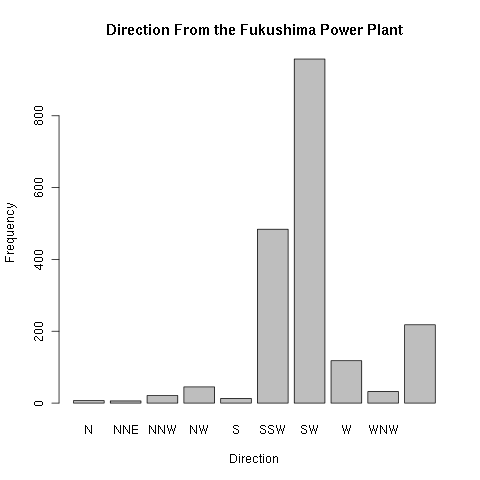
\includegraphics[width=8cm]{img/fukushimaDirectionBarPlot}
  \end{center}

\end{frame}

\begin{frame}
  \frametitle{Direction - Pareto Chart}

  \begin{center}
    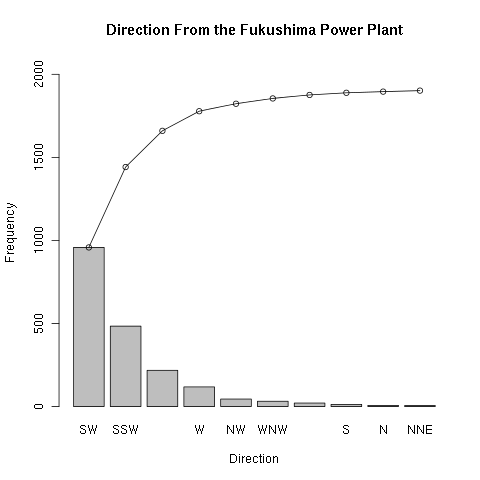
\includegraphics[width=8cm]{img/fukushimaParetoDirection}
  \end{center}

\end{frame}

\begin{frame}
  \frametitle{Radiation Data}

  \begin{center}
    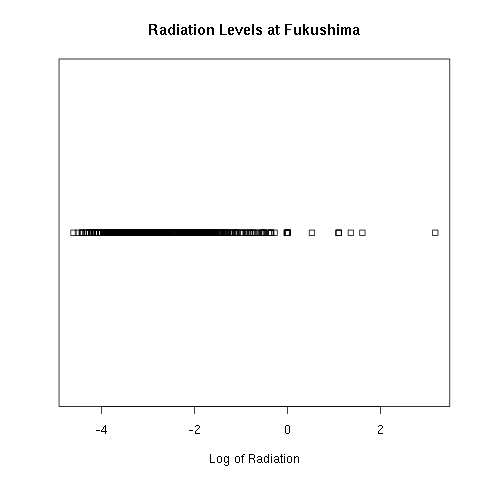
\includegraphics[width=8cm]{img/logFukushimaGamma}
  \end{center}  

\end{frame}

\begin{frame}
  \frametitle{Radiation Data}

  \begin{center}
    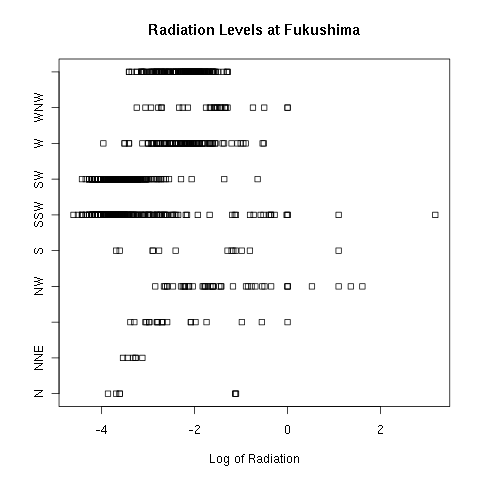
\includegraphics[width=8cm]{img/logFukushimaGammaByDirection}
  \end{center}  

\end{frame}


% LocalWords:  Clarkson pausesection hideallsubsections Cuby Webworks Webwork
% LocalWords:  ResponseCard Fukushima


%\part{}
\lecture{More Frequencies}{more-frequencies}


\title{More Graphical Views of Frequency}
\subtitle{Section 2.2}

\author{Kelly Black}
\institute{Clarkson University}
\date{16 January 2012}

\begin{frame}
  \titlepage
\end{frame}

\begin{frame}
  \frametitle{Outline}
  \tableofcontents[pausesection,hideallsubsections]
\end{frame}


\section{Clicker Question}


\begin{frame}
  \frametitle{Question:}

  Which plot below represents the Pareto chart for the following data:

    A, A, C, B, B, B, D

    \begin{tabular}{ccc}
      A: 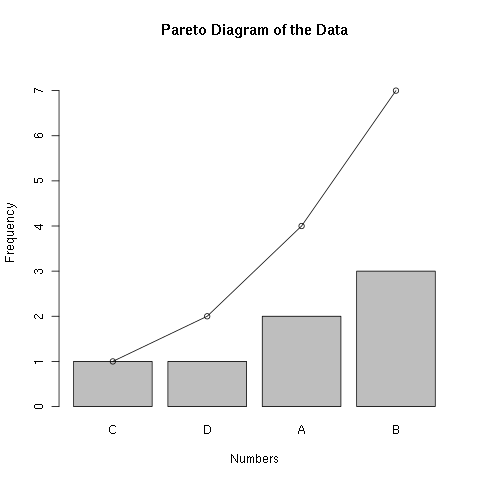
\includegraphics[width=3cm]{img/paretoQuizW1D2-a} &
      B: 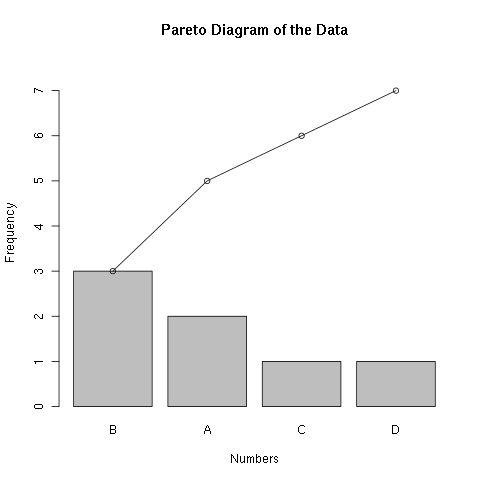
\includegraphics[width=3cm]{img/paretoQuizW1D2-b} &
      C: 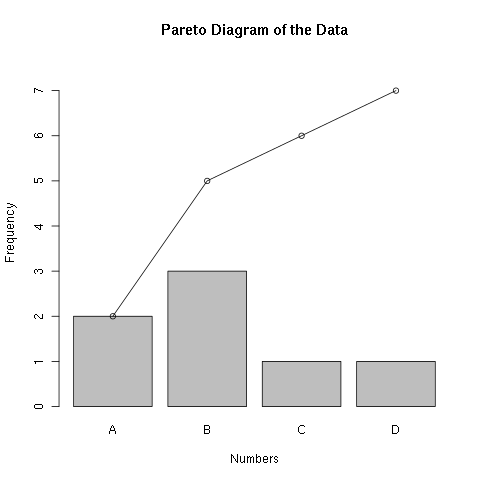
\includegraphics[width=3cm]{img/paretoQuizW1D2-c}
  \end{tabular}
  \uncover<2->{
    The answer is B
  }

\end{frame}


\section{Frequency}
\section{Histograms}

\begin{frame}
  \frametitle{Histograms}

  Things to look for in a histogram:\\
  \begin{itemize}
  \item Spread
  \item Symmetry
  \item Evenness or variedness
  \item Skewness
  \item Mode
  \end{itemize}

\end{frame}


\begin{frame}
  \frametitle{Symmetry}

  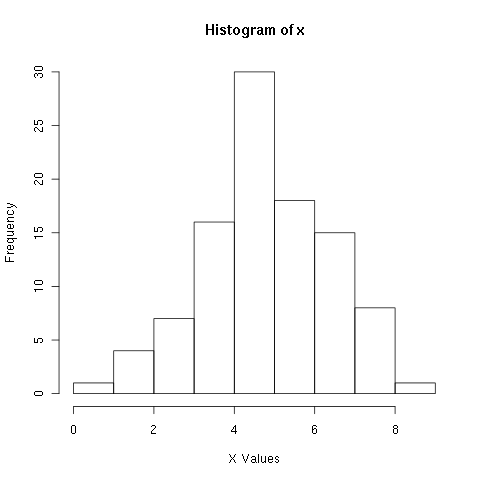
\includegraphics[width=7cm]{img/symmetricW1D2}

\end{frame}

\begin{frame}
  \frametitle{Uniformity}

  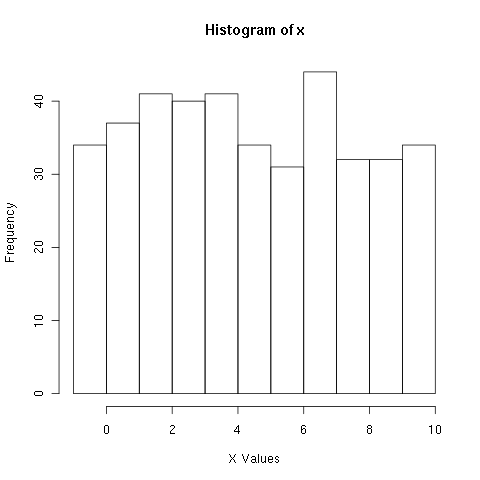
\includegraphics[width=7cm]{img/uniformW1D2}

\end{frame}


\begin{frame}
  \frametitle{Skewed Right}

  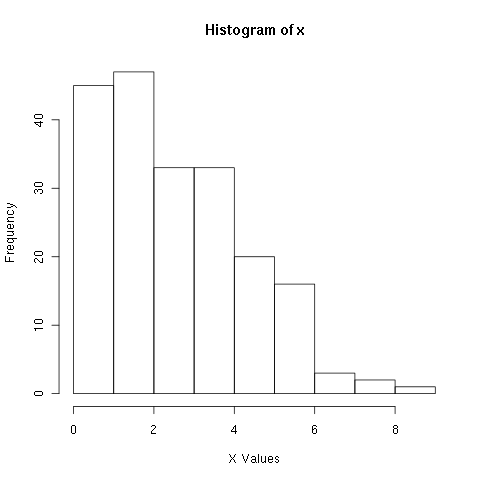
\includegraphics[width=7cm]{img/skewedRightW1D2}

\end{frame}


\begin{frame}
  \frametitle{Skewed Left}

  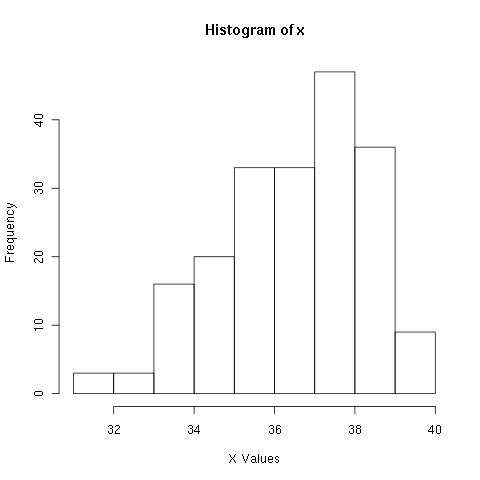
\includegraphics[width=7cm]{img/skewedLeftW1D2}

\end{frame}


\begin{frame}
  \frametitle{Bimodal}

  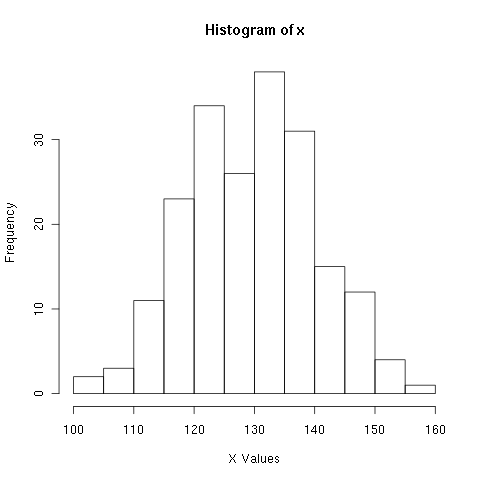
\includegraphics[width=7cm]{img/bimodalW1D2}

\end{frame}


\section{Cumulative Frequency}


\begin{frame}
  \frametitle{Cumulative Frequency}

  \begin{definition}
    The Cumulative Frequency is the frequncy of occurances for each
    result \textbf{less} than the given value.
  \end{definition}

\end{frame}


% LocalWords:  Clarkson pausesection hideallsubsections ccc



\lecture{Central Tendencies}{central-tendencies}
\part{Central Tendencies}

\title{Center and Spread of Data}
\subtitle{Sections 2.3 and 2.4}

\author{Kelly Black}
\institute{Clarkson University}
\date{18 January 2012}

\begin{frame}
  \titlepage
\end{frame}

\begin{frame}
  \frametitle{Outline}
  \tableofcontents[pausesection,hideallsubsections,part=1]
\end{frame}


\section{Clicker Question}


\begin{frame}
  \frametitle{Find The Average}
  (Use channel 42)

  \vfill 

  \begin{tabular}{lll}
    3, & 5, & -2
  \end{tabular}

  \vfill

  \begin{tabular}{l@{\hspace{3em}}l@{\hspace{3em}}l}
    a: 2 & b: -2 & c: 5
  \end{tabular}

  \vfill


\end{frame}


\section{Center of Data}


\begin{frame}
  \frametitle{Center of Data}

  Given data:
  \begin{eqnarray*}
    x_1, ~ x_2, ~ x_3, ~ \ldots ~,x_n.
  \end{eqnarray*}

  \begin{definition}
    The sample mean of the data is 
    \begin{eqnarray*}
      \bar{x} & = & \frac{x_1+x_2+\cdots+x_n}{n}.
    \end{eqnarray*}
  \end{definition}

  \begin{definition}
    The median is the number for which half the data is smaller than
    it and half is larger that it.
  \end{definition}
  

\end{frame}


\section{Spread of Data}


\begin{frame}
  \frametitle{Spread of Data}

  Given data:
  \begin{eqnarray*}
    x_1, ~ x_2, ~ x_3, ~ \ldots ~,x_n.
  \end{eqnarray*}

  \begin{definition}
    The range is the biggest number minus the smallest number.
  \end{definition}


  \begin{definition}
    The sample variation of the data is 
    \begin{eqnarray*}
      s^2 & = & \frac{(x_1-\bar{x})^2+(x_2-\bar{x})^2+\cdots+(x_n-\bar{x})^2}{n-1}.
    \end{eqnarray*}
  \end{definition}

  \begin{definition}
    The sample standard deviation of the data is the square root of
    the sample variation.
  \end{definition}


\end{frame}


\begin{frame}
  \frametitle{Clicker Quiz}
  (Use channel 42)

  Find the standard deviation of the following data set:
  \vfill 

  \begin{tabular}{llll}
    3, & 5, & 2, & 4
  \end{tabular}

  \vfill

  \begin{tabular}{l@{\hspace{3em}}l@{\hspace{3em}}l}
    a: 1.667 & b: 1.180 & c: 1.291
  \end{tabular}

  \vfill

  

\end{frame}





% LocalWords:  Clarkson pausesection hideallsubsections




% %%%%%%%%%%%%%%%%%%%%%%%%%%%%%%%%%%%%%%%%%%%%%%%%%%%%%%%%%%%%


\lecture{Measures Of Position}{measures-of-position}
\part{Measures Of Position}


\title{Measures Of Position}
\subtitle{Where are you?}

\author{Kelly Black}
\institute{Clarkson University}
\date{20 January 2012}

\begin{frame}
  \titlepage
\end{frame}

\begin{frame}
  \frametitle{Outline}
  \tableofcontents[pausesection,hideallsubsections,part=1]
\end{frame}


\section{Clicker Quiz}


\begin{frame}
  \frametitle{Clicker Quiz}

  \vfill
  Find the third quartile of the following data set:\\
  \begin{tabular}{llllll}
    28, & 17, & 12, & 20, & 21, & 18
  \end{tabular}

  \vfill

  \begin{tabular}{l@{\hspace{3em}}l@{\hspace{3em}}l}
    A: 17 & B: 19 & C: 21
  \end{tabular}

  \vfill

\end{frame}




\section{Percentiles}

\begin{frame}
  \frametitle{Percentiles}

  \begin{definition}
    The P\textsuperscript{th} percentile is the data point for which P\%
    of the numbers are smaller than it.
  \end{definition}

\end{frame}

\begin{frame}
  \frametitle{Percentiles}

%  \begin{eqnarray*}
%    \begin{array}{lllll}
%      x_1 & x_2 & x_3 & \cdots & x_n \\
%    \end{array}
%  \end{eqnarray*}

  \newcount\xnum
  \newcount\xnumpos
  \only<1>
  {
    \begin{picture}(500,100)(0,0)
      \multiput(10,90)(20, 0){15}{\line(1,0){15}}
      \xnum=1
      \xnumpos=12
      \loop
      \put(\xnumpos,95){$x_{{\the\xnum}}$}
      \advance\xnumpos by 20
      \ifnum\xnum < 15 \advance\xnum by 1
      \repeat
    \end{picture}
  }

  \only<2>
  {
    \begin{picture}(310,100)(0,0)
      \multiput(10,90)(20, 0){15}{\line(1,0){15}}
      \xnum=1
      \xnumpos=12
      \loop
      \put(\xnumpos,95){$x_{{\the\xnum}}$}
      \advance\xnumpos by 20
      \ifnum\xnum < 15 \advance\xnum by 1
      \repeat
      \put(10,0){\line(0,1){80}}
      \put(310,0){\line(0,1){80}}
      \put(110,20){\vector(-1,0){100}}
      \put(210,20){\vector( 1,0){100}}
      \put(120,15){Width=n Items}
    \end{picture}
  }

  \only<3>
  {
    \begin{picture}(310,100)(0,0)
      \multiput(10,90)(20, 0){15}{\line(1,0){15}}
      \xnum=1
      \xnumpos=12
      \loop
      \put(\xnumpos,95){$x_{{\the\xnum}}$}
      \advance\xnumpos by 20
      \ifnum\xnum < 15 \advance\xnum by 1
      \repeat
      \put(10,0){\line(0,1){80}}
      \put(310,0){\line(0,1){80}}
      \put(110,20){\vector(-1,0){100}}
      \put(210,20){\vector( 1,0){100}}
      \put(120,15){Width=n Items}

      \put(250,50){\line(0,1){40}}
      \put(80,60){\vector(-1,0){70}}
      \put(180,60){\vector( 1,0){70}}
      \put(85,55){P Percent of Width}

    \end{picture}
  }

  \vfill
  
\end{frame}

\begin{frame}
  \frametitle{Percentiles}

    \begin{picture}(310,100)(0,0)
      \multiput(10,90)(20, 0){15}{\line(1,0){15}}
      \xnum=1
      \xnumpos=12
      \loop
      \put(\xnumpos,95){$x_{{\the\xnum}}$}
      \advance\xnumpos by 20
      \ifnum\xnum < 15 \advance\xnum by 1
      \repeat
      \put(10,0){\line(0,1){80}}
      \put(310,0){\line(0,1){80}}
      \put(110,20){\vector(-1,0){100}}
      \put(210,20){\vector( 1,0){100}}
      \put(120,15){Width=n Items}

      \put(250,50){\line(0,1){40}}
      \put(70,60){\vector(-1,0){60}}
      \put(190,60){\vector( 1,0){60}}
      \put(75,55){j/n items = k\textsuperscript{th} percent}

    \end{picture}


    \begin{eqnarray*}
      P & = & \frac{k}{100}, \\
      \frac{j}{n} & = & \frac{k}{100}, \\
      \Rightarrow j & = & \frac{nk}{100}.
    \end{eqnarray*}

\end{frame}

\begin{frame}
  \frametitle{Example}

  \vfill 

  Find the 85\textsuperscript{th} percentile for the following data:

  \vfill

  \only<1>
  {
    89, 85, 97 106, 94, 100, 92, 120, 92, 97, 89, 90, 103, 86, 106, 112, 100, 92, 84,
    97, 103, 91, 104, 91, 104
  }

  \only<2>
  {
    Sort it: \\
    84, 85, 86, 89, 89, 90, 91, 91, 92, 92, 92, 94, 97, 97, 97, 100,
    100, 103, 103, 104, 104, 106, 106, 112, 120
  }

  \only<3>
  {
    Sort it: \\
    84, 85, 86, 89, 89, 90, 91, 91, 92, 92, 92, 94, 97, 97, 97, 100,
    100, 103, 103, 104, \underline{104}, \underline{106}, 106, 112, 120
  }


  \vfill

  (There are 25 data points.)

  \vfill

\end{frame}

\begin{frame}
  \frametitle{Clicker Quiz}

  \vfill

  Find the 30\textsuperscript{th} percentile for the following data:

  185, 196, 214, 199, 199, 204


  \vfill

  \begin{tabular}{l@{\hspace{3em}}l@{\hspace{3em}}l}
    A: 198 & B: 198 $\frac{2}{5}$ & C: 199
  \end{tabular}



\end{frame}

\section{Box Plots}

\begin{frame}
  \frametitle{Box Plots}

  \vfill 

  Find the five point summary for the following data:

  \vfill

  \only<1>
  {
    89, 85, 97 106, 94, 100, 92, 120, 92, 97, 89, 90, 103, 86, 106, 112, 100, 92, 84,
    97, 103, 91, 104, 91, 104

    \vfill
  }

  \only<2>
  {
    Sort it: \\
    84, 85, 86, 89, 89, 90, 91, 91, 92, 92, 92, 94, 97, 97, 97, 100,
    100, 103, 103, 104, 104, 106, 106, 112, 120

    Five point summary: \\
    \begin{tabular}{lllll}
     Min. & 1st Qu. & Median    & 3rd Qu. &   Max. \\
     84   & 91      & 97        & 103     & 120
    \end{tabular}


  }

  \vfill

\end{frame}


\begin{frame}
  \frametitle{Box Plots}

    Five point summary: \\
    \begin{tabular}{lllll}
     Min. & 1st Qu. & Median    & 3rd Qu. &   Max. \\
     84   & 91      & 97        & 103     & 120
    \end{tabular}

    \begin{center}
      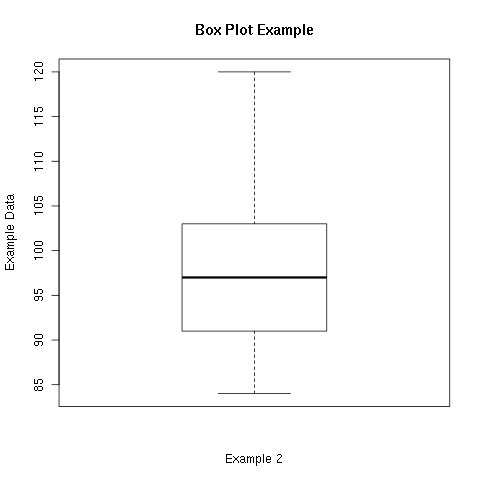
\includegraphics[width=6cm]{img/boxplotExample1}
    \end{center}

\end{frame}



\begin{frame}
  \frametitle{Z-Score}

  \begin{definition}
    Given a set of data,
    \begin{eqnarray*}
      x_1,~x_2,~x_3,\ldots,x_n,
    \end{eqnarray*}
    with sample mean $\bar{x}$ and standard deviation $s$ the
    $z$-score for a number, $x$, is
    \begin{eqnarray*}
      z & = & \frac{x-\bar{x}}{s}.
    \end{eqnarray*}
  \end{definition}

\end{frame}


% LocalWords:  Clarkson pausesection hideallsubsections



\lecture{Introduction to Bivariate Data}{introduction-to-bivariate-data}
\part{Introduction to Bivariate Data}

\title{Introduction to Bivariate Data}
\subtitle{Qualitative and Quantitative Data}

\author{Kelly Black}
\institute{Clarkson University}
\date{23 January 2012}

\begin{frame}
  \titlepage
\end{frame}

\begin{frame}
  \frametitle{Outline}
  \tableofcontents[pausesection,hideallsubsections,part=1]
\end{frame}


\section{Clicker Quiz}


\begin{frame}
  \frametitle{Clicker Quiz}

  We have a data set and find a sample mean of 2.5 and a sample
  standard deviation of 6.1. What is the $z$-statistic for $x=2.7$.

  \begin{tabular}{l@{\hspace{3em}}l@{\hspace{3em}}l@{\hspace{3em}}l}
    A: -1.220 & B: -0.033 & C: 0.033 & D: 1.220
  \end{tabular}


\end{frame}




\section{Bivariate Data}

\begin{frame}
  \frametitle{Bivariate Data}

  \begin{eqnarray*}
    \begin{array}{l|l}
      x      & y \\ \hline 
      x_1    & y_1 \\
      x_2    & y_2 \\
      \vdots & \vdots \\
      x_n    & y_n
    \end{array}
  \end{eqnarray*}
\end{frame}

\section{Qualitative Data}

\begin{frame}
  \frametitle{Cross Tabular Tables}

  \begin{tabular}{ll}
    $Q_{1}$ & $Q_{2}$ \\ \hline
    A & Y \\
    B & Y \\
    B & N \\
    B & N \\
    A & N \\
    B & N
  \end{tabular}

  \uncover<2->
  {
    \begin{tabular}{l|l|l|l}
      $Q_1 \backslash Q_2$ & Y & N & Row Total \\
      A & 1 & 1 & 2 \\ \hline
      B & 1 & 3 & 4 \\ \hline
      Col. Total & 2 & 4 & 6
    \end{tabular}
  }

\end{frame}


\begin{frame}
  \frametitle{Clicker Quiz}


  Determine the table for this data with the row percentages:

  \begin{columns}
    \column{.25\textwidth}

  \begin{tabular}{l|l}
    $Q_{1}$ & $Q_{2}$ \\ \hline
    a & d \\
    a & e \\
    b & e \\
    a & d \\
    b & e \\
    a & d
  \end{tabular}


    \column{.75\textwidth}

    1:
    \begin{tabular}{l|l|l|l}
      $Q_1 \backslash Q_2$ & d & e & Row \\
      a & 3/4 & 1/4 & 1.0 \\ \hline
      b & 0.0 & 1.0 & 1.0 \\ \hline
      Col.  & 3/6 & 3/6 & 1.0
    \end{tabular}

    \rule{5cm}{0.05cm}

    2:
    \begin{tabular}{l|l|l|l}
      $Q_1 \backslash Q_2$ & d & e & Row  \\
      a & 1.0 & 1/3 & 4/6 \\ \hline
      b & 0.0 & 2/3 & 2/6 \\ \hline
      Col.  & 1.0 & 1.0 & 1.0
    \end{tabular}

    \rule{5cm}{0.05cm}

    3:
    \begin{tabular}{l|l|l|l}
      $Q_1 \backslash Q_2$ & d & e & Row  \\
      a & 1.0 & 0.0 & 1.0 \\ \hline
      b & 1/3 & 2/3 & 1.0 \\ \hline
      Col.  & 3/5 & 2/5 & 1.0
    \end{tabular}


  \end{columns}

\end{frame}

\section{Quantitative Data}

\begin{frame}
  \frametitle{Quantitative Data}

  \begin{eqnarray*}
    \begin{array}{l|l}
      X & Y \\ \hline
      x_1 & y_1 \\
      x_2 & y_2 \\
      x_3 & y_3 \\
      x_4 & y_4 \\
      \vdots & \vdots \\
      x_n & y_n
  \end{array}
\end{eqnarray*}

\end{frame}

\begin{frame}
  \frametitle{Example}

  \begin{columns}
    \column{.25\textwidth}

  \begin{eqnarray*}
    \begin{array}{r|r}
      X & Y \\ \hline
      3 & 6 \\
      2 & 2 \\
      -1 & -3 \\
      4 & 4 \\
      2 & 3
    \end{array}
  \end{eqnarray*}


    \column{.75\textwidth}

  \only<2->
  {
    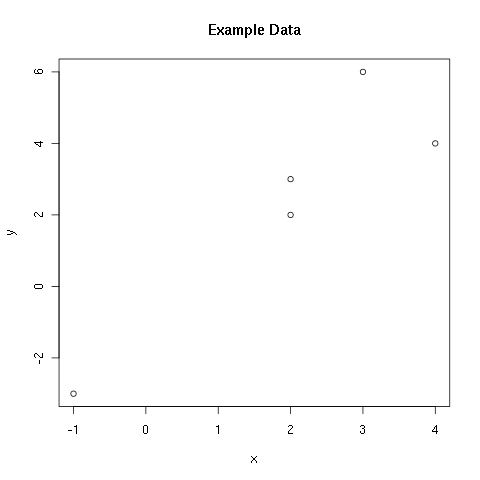
\includegraphics[width=7cm]{img/simpleBivariateExample}
  }


  \end{columns}


\end{frame}


% LocalWords:  Clarkson pausesection hideallsubsections Bivariate



\lecture{Correlation and Regression}{correlation-regression}
\section{Correlation and Regression}

\title{Correlation and Linear Regression}
\subtitle{Is a Straight Line Appropriate?}

\author{Kelly Black}
\institute{Clarkson University}
\date{25 January 2012}

\begin{frame}
  \titlepage
\end{frame}

\begin{frame}
  \frametitle{Outline}
  \tableofcontents[pausesection,hideothersubsections,sectionstyle=show/hide]
\end{frame}


\subsection{Clicker Quiz}


\begin{frame}{Clicker Quiz}

Determine if the following relationship is a ``positive relationship''
or a ``negative relationship'' between the two variables.

\begin{center}
  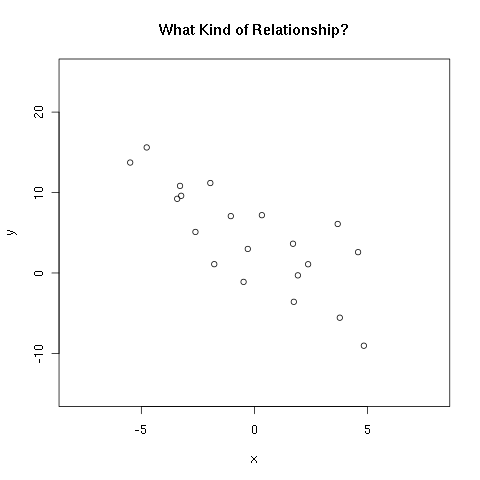
\includegraphics[width=6cm]{img/week2Day3ClickerQuizNeg}
\end{center}

\begin{tabular}{l@{\hspace{3em}}l}
  A: Positive & B: Negative
\end{tabular}


\end{frame}


\begin{frame}{Positive vs. Negative Relationships}

  \begin{columns}
    \column{.5\textwidth}
    Positive Relationship: \\
    \centerline{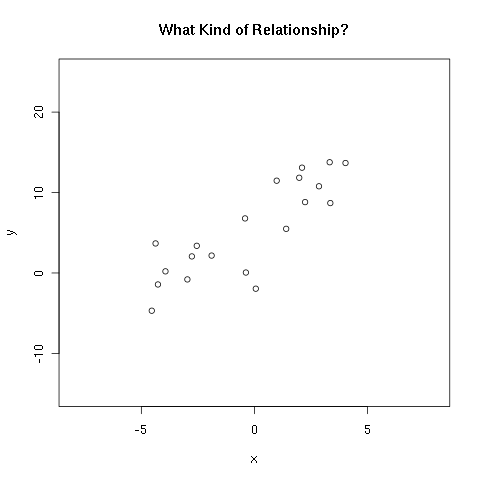
\includegraphics[width=5cm]{img/week2Day3ClickerQuizPos}}
    \column{.5\textwidth}
    Negative Relationship: \\
    \centerline{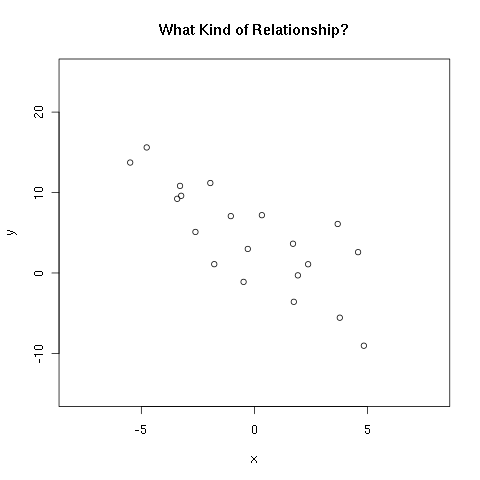
\includegraphics[width=5cm]{img/week2Day3ClickerQuizNeg}}
  \end{columns}
  
\end{frame}



\subsection{Correlation}

\begin{frame}{Correlation}

  \hspace*{-3em}
  \begin{tabular}{rrr}
    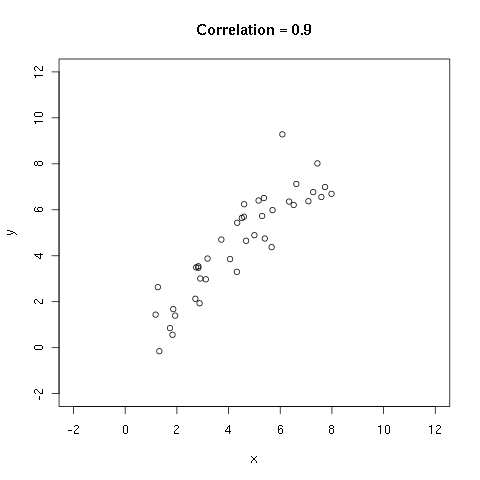
\includegraphics[height=4cm]{img/correlation09} & 
    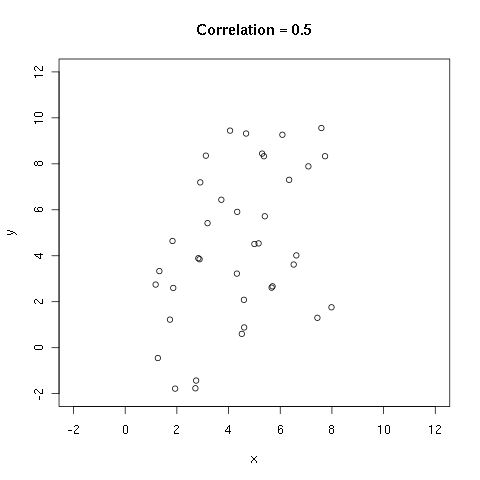
\includegraphics[height=4cm]{img/correlation05} &
    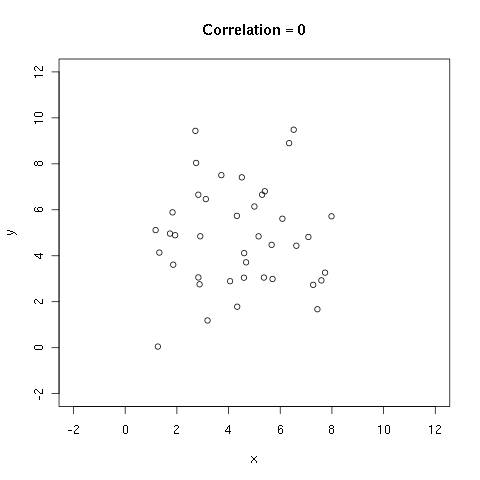
\includegraphics[height=4cm]{img/correlation0} \\
    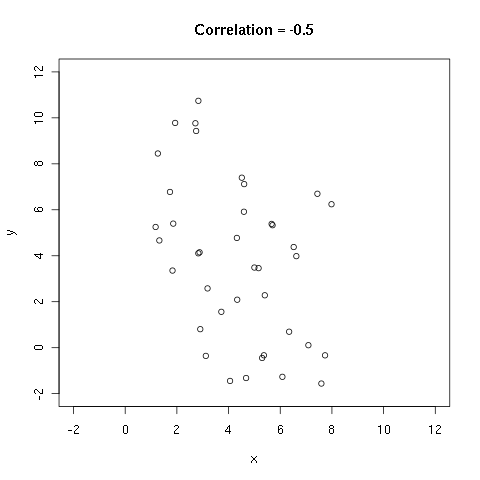
\includegraphics[height=4cm]{img/correlation-05} &
    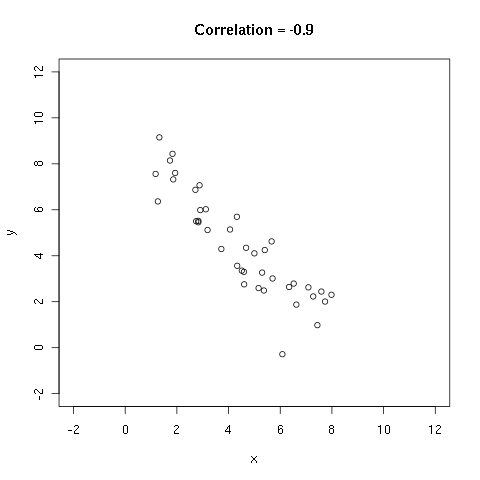
\includegraphics[height=4cm]{img/correlation-09}
  \end{tabular}


\end{frame}


\begin{frame}{Calculating the Correlation}

  First define the following sums:
  \begin{eqnarray*}
    S_{xx} & = & (x_1-\bar{x})^2 + (x_2-\bar{x})^2 + \cdot + (x_n-\bar{x})^2, \\
    S_{yy} & = & (y_1-\bar{y})^2 + (y_2-\bar{y})^2 + \cdot + (y_n-\bar{y})^2, \\
    S_{xy} & = & (x_1-\bar{x}) + (x_2-\bar{x}) + \cdot + (x_n-\bar{x}), \\
  \end{eqnarray*}

  \uncover<2->
  {
    
    \begin{definition}
      The sample correlation coefficient is defined to be
      \begin{eqnarray*}
        r & = & \frac{S_{xy}}{\sqrt{S_{xx} S_{yy}}}.
      \end{eqnarray*}
    \end{definition}

  }
  
\end{frame}



\begin{frame}{Example}
  
  \begin{columns}
    \column{.25\textwidth}
    \begin{tabular}{l|l}
      $x$ & $y$ \\ \hline
      -1 & -1 \\
      0 & 1 \\
      1 & 2 \\
      2 & 4
    \end{tabular}

    \column{.75\textwidth}
    
    \uncover<2->
    {
      \centerline{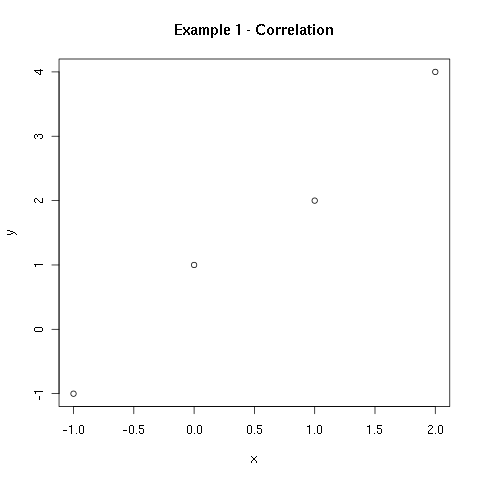
\includegraphics[width=6cm]{img/week2-Day3Correlation}}
    }

    \end{columns}

\end{frame}


\subsection{Linear Regression}


\begin{frame}{Clicker Quiz 2}
  
  \begin{columns}
    \column{.25\textwidth}
    \begin{tabular}{l|l}
      $x$ & $y$ \\ \hline
      -1 & -1 \\
      0 & 1 \\
      1 & 2 \\
      2 & 4
    \end{tabular}

    \column{.75\textwidth}

    What is $S_{yy}$?

    \begin{tabular}{l@{\hspace{3em}}l@{\hspace{3em}}l}
      A: 5  & B: 8.5 & C: 16.75
    \end{tabular}


    \end{columns}

\end{frame}


\begin{frame}{Example}
  
  \begin{columns}
    \column{.25\textwidth}
    \begin{tabular}{l|l}
      $x$ & $y$ \\ \hline
      -1 & -1 \\
      0 & 1 \\
      1 & 2 \\
      2 & 4
    \end{tabular}

    \column{.75\textwidth}
    
    \only<2>
    {
      \centerline{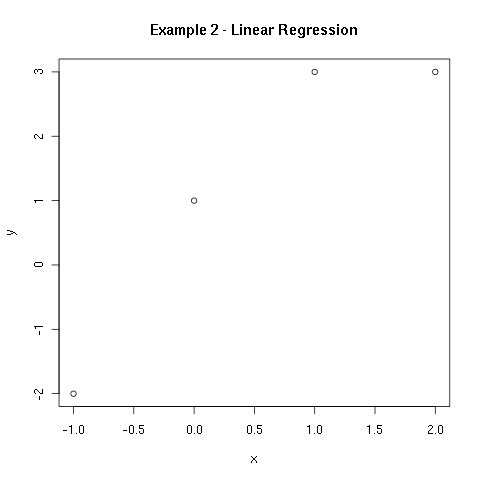
\includegraphics[width=6cm]{img/week2-Day3-Regression1}}
    }

    \only<3>
    {
      \centerline{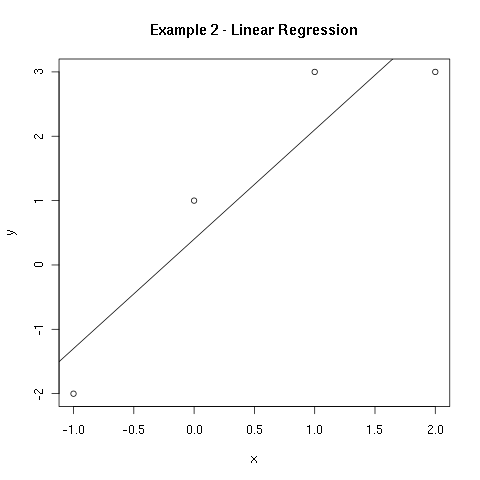
\includegraphics[width=6cm]{img/week2-Day3-Regression2}}
    }


    \end{columns}

\end{frame}




% LocalWords:  Clarkson pausesection hideallsubsections rrr yy xy



% %%%%%%%%%%%%%%%%%%%%%%%%%%%%%%%%%%%%%%%%%%%%%%%%%%%%%%%%%%%%


\lecture{Introduction to Probability}{intro-to-probability}
\section{Introduction to Probability}

\title{Probability}
\subtitle{What are the chances?}

%\author{Kelly Black}
%\institute{Clarkson University}
\date{27 January 2012}

\begin{frame}
  \titlepage
\end{frame}

\begin{frame}
  \frametitle{Outline}
  \tableofcontents[pausesection,hideothersubsections,sectionstyle=show/hide]
\end{frame}


\subsection{Clicker Quiz}


\begin{frame}
  \frametitle{Clicker Quiz}

  If I flip a fair coin ten times how many tails will I get?

  \begin{tabular}{l@{\hspace{3em}}l@{\hspace{3em}}l@{\hspace{3em}}l}
    A: 4 & B: 5 & C: 6 & D: I do not know
  \end{tabular}


\end{frame}




\subsection{Clicker Exercise}

\begin{frame}
  \frametitle{Clicker Exercise}

  Flip a coin 3 times. How many tails did you get?

  \begin{tabular}{l@{\hspace{3em}}l@{\hspace{3em}}l@{\hspace{3em}}l}
  A: 0 & B: 1 & C: 2 & D: 3
  \end{tabular}
  

\end{frame}

\subsection{Events}

\begin{frame}
  \frametitle{Events}

  \begin{definition}
    An event is a possible outcome from an experiment.
  \end{definition}

\end{frame}


\begin{frame}
  \frametitle{Sample Space}

  \begin{definition}
    The sample space is the collection of all possible events.
  \end{definition}

\end{frame}


\begin{frame}
  \frametitle{Sample Space}

  There are two ways to visualize the sample space:
  \begin{itemize}
  \item Venn Diagram
  \item Tree Diagram
  \end{itemize}

\end{frame}


\begin{frame}{Clicker Quiz}
  A couple has a child. Two years later they have another child. What
  is the probability that they have one girl and one boy?

  \begin{tabular}{l@{\hspace{3em}}l@{\hspace{3em}}l@{\hspace{3em}}l}
    A: 0 & B: 1/4 & C: 1/2 & D: 1
  \end{tabular}


\end{frame}

\subsection{Properties of Probabilities}

\begin{frame}{Properties of Probabilities}

  Suppose that A is an event in the sample space, then
  \begin{eqnarray*}
    \begin{array}{rcccl}
      0 & \leq & P(A) & \leq & 1
    \end{array}
  \end{eqnarray*}
  
\end{frame}

% LocalWords:  Clarkson pausesection hideallsubsections



\lecture{Conditional Probability}{conditional-probability}
\part{Conditional Probability}

\title{Conditional Probability}
\subtitle{What do you know?}

\author{Kelly Black}
\institute{Clarkson University}
\date{30 January 2012}

\begin{frame}
  \titlepage
\end{frame}

\begin{frame}
  \frametitle{Outline}
  \tableofcontents[pausesection,hideallsubsections,part=1]
\end{frame}


\section{Clicker Quiz}


\begin{frame}
  \frametitle{Clicker Quiz}

  I have a bag with eight marbles. Five marbles are red and three are
  blue. I pull one marble out at random. What is the probability that
  it is red?

  \begin{tabular}{l@{\hspace{3em}}l@{\hspace{3em}}l@{\hspace{3em}}l}
    A: 3/8 & B: 5/8 & C: 1
  \end{tabular}


\end{frame}




\section{Conditional Probability}

\begin{frame}
  \frametitle{Example 1 (from 4.10 in the book)}

  1000 voters are polled in the 2008 election. We get the following
  information: \\
  \only<1>
  {
    \begin{tabular}{l|l|l|l}
      Education & Obama & McCain & Others  \\ \hline
      No H.S. Diploma & 19 & 20 & 1   \\
      H.S. Diploma only & 114 & 103 & 3 
    \end{tabular}
  }
  \only<2->
  {
    \begin{tabular}{l|l|l|l|l}
      Education & Obama & McCain & Others & Total \\ \hline
      No H.S. Diploma & 19 & 20 & 1 & 40 \\
      H.S. Diploma only & 114 & 103 & 3 & 220 \\ \hline
      Total & 133 & 123 & 4 & 260
    \end{tabular}
  }



\end{frame}


\begin{frame}{Clicker Quiz}


  A bowl has candy. Eight of the candies are chocolate, and of the
  chocolates three have red wrappers while the rest have silver
  wrappers. Twelve of the candies are hard candy, and of the hard
  candies four have red wrappers while the rest have silver
  wrappers. I pull out one candy at random, and it is a
  chocolate. What is the probability that it has a red wrapper?

  \begin{tabular}{l@{\hspace{3em}}l@{\hspace{3em}}l@{\hspace{3em}}l}
    A: 4/12 & B: 3/8 & C: 5/8 & D: 8/12
  \end{tabular}

  
\end{frame}


\begin{frame}
  \frametitle{Conditional Probability}

  \begin{definition}
    The probability that A occurs given that I know that B occured is
    defined to be 
    \begin{eqnarray*}
      p(A|B) & = & \frac{p(A \mathrm{~and~} B)}{p(B)}, \\
      \mathrm{or~} 
      p(B) p(A|B)  &  =  & p(A \mathrm{~and~} B).
    \end{eqnarray*}
  \end{definition}

\end{frame}


\begin{frame}{Example 2}

  I have a bag with eight marbles. Five marbles are red and three are
  blue. I pick two, one after the other without replacing them. What
  is the probability that I pull out a red and then a blue marble?
  
\end{frame}

\section{Compliment}

\begin{frame}{Compliment}

  \begin{definition}
    Suppose $A$ is an event. Then all of the events not in A are denoted
    by $\bar{A}$. 

    Other notations:
    \begin{eqnarray*}
      \bar{A},~A',~A^c
    \end{eqnarray*}
  \end{definition}


\end{frame}


\begin{frame}{Probabilities of Compliments}
  
  \begin{eqnarray*}
    1 & = & p(A) + p(\bar{A}), \\
    p(A) & = & 1 - p(\bar{A}).
  \end{eqnarray*}

\end{frame}


% LocalWords:  Clarkson pausesection hideallsubsections Obama




% %%%%%%%%%%%%%%%%%%%%%%%%%%%%%%%%%%%%%%%%%%%%%%%%%%%%%%%%%%%%

\include{week4-Day1}


\lecture{Independence And Mutual Exclusion}{indepence-and-mutual-exclusion}
\part{Independence And Mutual Exclusion}

\title{Independence And Mutual Exclusion}
\subtitle{Stuff We Already Did}

\author{Kelly Black}
\institute{Clarkson University}
\date{3 Feb 2012}

\begin{frame}
  \titlepage
\end{frame}

\begin{frame}
  \frametitle{Outline}
  \tableofcontents[pausesection,hideallsubsections,part=1]
\end{frame}


\section{Clicker Quiz}


\begin{frame}
  \frametitle{Clicker Quiz}

  If $p(A)=0.3$, $p(B)=0.4$, and $p(A\mathrm{~or~}B)=.37$ what is
  $p(A\mathrm{~and~}B)$?

  \vfill

  \begin{tabular}{l@{\hspace{3em}}l@{\hspace{3em}}l}
    A: .11 & B: 12 & C: .33
  \end{tabular}

  \vfill
  \vfill
  \vfill

\end{frame}




\section{Example}

\begin{frame}
  \frametitle{Example 1}

  I flip a coin two times. What is the probability that I get a tails
  on the second flip?

  \vfill


\end{frame}


\section{Mutually Exclusive Events}

\begin{frame}
  \frametitle{Mutual Exclusion}

  \begin{definition}
    Two sets are \textit{mutually exclusive} if they have nothing in
    common.
  \end{definition}

\end{frame}


\begin{frame}{Example 2}
  
  I have a bag with six red marbles and two blue marbles. I draw two
  without replacement. What is the probability that the second marble
  is red?

  \vfill

\end{frame}

\section{Independent Events}

\begin{frame}
  \frametitle{Independence}

  \begin{definition}
    Two events are independent if 
    \begin{eqnarray*}
      p(A|B) & = & p(A).
    \end{eqnarray*}

    This is equivalent to requiring that
    \begin{eqnarray*}
      p(B|A) & = & p(B).
    \end{eqnarray*}

  \end{definition}

\end{frame}



\begin{frame}{Example 3}

  Suppose that $p(A)=0.6$, $p(B)=0.3$, and $p(A\mathrm{~and~}B)=.2$
  Are they independent?

  \vfill

  
\end{frame}



\begin{frame}{Example 4}

  Suppose that $p(A)=0.6$, $p(B)=0.3$, and $p(A\mathrm{~and~}B)=.18$
  Are they independent?

  \vfill

  
\end{frame}


\begin{frame}{Example 5}
  An industrial process is established to produce items. About five
  percent of the items are defective under this process. Each item is
  inspected, and fifteen percent of the defective items are not caught
  in the inspection. About three percent of the good items are
  classified as defective.

  \begin{itemize}
  \item What percentage of the items that are sold are defective?
  \item I pick a part at random. That part is classified as
    defective. What is the probability that it is actually defective?
  \end{itemize}

  \vfill

\end{frame}


\begin{frame}{Example 6}

  A brokerage firm has a system that can execute a sell request in
  within 0.08 seconds about 85\% of the time. Of the requests that
  occur within 0.08 seconds about 75\% meet the projected cost
  level. Of the requests that do not occur within 0.08 seconds about
  65\% meet the projected cost level.

  What is the proportion of requests that will meet the projected cost
  levels?

  \vfill
  
\end{frame}




% LocalWords:  Clarkson pausesection hideallsubsections



% %%%%%%%%%%%%%%%%%%%%%%%%%%%%%%%%%%%%%%%%%%%%%%%%%%%%%%%%%%%%



\newcommand{\arrayTwo}[4]{
  \left[
  \begin{array}{rr}
    #1 & #2 \\
    #3 & #4
  \end{array}
  \right]
}

\newcommand{\vecTwo}[2]{
  \left[
  \begin{array}{r}
    #1 \\  #2
  \end{array}
  \right]
}


\newcommand{\stateTwo}[2]{
  \begin{array}{rr}
    \mbox{\fontsize{6}{6}\selectfont $#1$} \\  \mbox{\fontsize{6}{6}\selectfont $#2$}
  \end{array}
}


\newcommand{\arrayThree}[9]{
  \left[
    \begin{array}{rrr}
      #1 & #2 & #3 \\
      #4 & #5 & #6 \\
      #7 & #8 & #9
    \end{array}
  \right]
}

\newcommand{\startRowOps}{
  \left[
    \begin{array}{rrr|r}
}

\newcommand{\oneRowOps}[4] {
      #1 & #2 & #3 & #4 \\
}

\newcommand{\stopRowOps}{
    \end{array}
  \right]
}


\newcommand{\vecThree}[3]{
  \left[
  \begin{array}{r}
    #1 \\  #2 \\ #3
  \end{array}
  \right]
}


\newcommand{\stateThree}[3]{
  \begin{array}{r}
    \mbox{\fontsize{6}{6}\selectfont $#1$} \\  
    \mbox{\fontsize{6}{6}\selectfont $#2$} \\ 
    \mbox{\fontsize{6}{6}\selectfont $#3$}
  \end{array}
}





\newcommand{\detTwo}[4]{
  \left|
  \begin{array}{rr}
    #1 & #2 \\
    #3 & #4
  \end{array}
  \right|
}



\newcommand{\detThree}[9]{
  \left|
    \begin{array}{rrr}
      #1 & #2 & #3 \\
      #4 & #5 & #6 \\
      #7 & #8 & #9
    \end{array}
  \right|
}




\newcommand{\startRowFour}{
  \left[
    \begin{array}{rrrr}
}

\newcommand{\oneRowFour}[4] {
      #1 & #2 & #3 & #4 \\
}





\lecture{Probability Examples}{probability-examples}
\section{Probability Examples}

\title{Probability Examples}
\subtitle{Try These}

%\author{Kelly Black}
%\institute{Clarkson University}
\date{6 February 2012}

\begin{frame}
  \titlepage
\end{frame}

\begin{frame}
  \frametitle{Outline}
  \tableofcontents[pausesection,hideothersubsections,sectionstyle=show/hide]
\end{frame}


\subsection{Examples}


\begin{frame}
  \frametitle{Example}


  $p(A)=.5$, $p(B)=.3$, $p(A\mathrm{~and~}B)=.2$. What is $p(A|B)$?

  \vfill

  \begin{tabular}{l@{\hspace{3em}}l@{\hspace{3em}}l}
    A: .33 & B: .40 & C: .67
  \end{tabular}

  \vfill
  \vfill
  \vfill


\end{frame}






\begin{frame}
  \frametitle{Example}

  A survey is conducted. Two of the questions resulted in the
  following two way table:

  \vfill

  \begin{tabular}{lllllll}
      & Very Bad & Bad  & Good & Very Good & No Opinion & \\
    A &  46 & 137 & 345 & 68 & 6 & \\
    B & 141 & 178 & 48  &  2 & 4 & \\
    No Opinion & 2 & 13 & 4 & 0 & 1 
  \end{tabular}

  \vfill

  Determine the value of $p(\mathrm{Bad}|A$)?

  \vfill

  \begin{tabular}{l@{\hspace{3em}}l@{\hspace{3em}}l}
    A: 137/328  & B: 137/602 & C: 328/602
  \end{tabular}

  \vfill
  \vfill
  \vfill

\end{frame}

\begin{frame}
  \frametitle{Example}

  A survey is conducted. Two of the questions resulted in the
  following two way table:

  \vfill

  \begin{tabular}{lllllll}
      & Very Bad & Bad  & Good & Very Good & No Opinion & \\
    A &  46 & 137 & 345 & 68 & 6 & \\
    B & 141 & 178 & 48  &  2 & 4 & \\
    No Opinion & 2 & 13 & 4 & 0 & 1 
  \end{tabular}

  \vfill

  Determine the value of $p(\mathrm{good}|B$)?

  \vfill

  \begin{tabular}{l@{\hspace{3em}}l@{\hspace{3em}}l}
    A: 373/393  & B: 48/373 & C: 48/397
  \end{tabular}

  \vfill
  \vfill
  \vfill

\end{frame}



\begin{frame}
  \frametitle{Example}

  A survey is conducted. Two of the questions resulted in the
  following two way table:

  \vfill

  \begin{tabular}{llllll|l}
      & Very Bad & Bad  & Good & Very Good & N.O. & Total \\ \hline
    A &  46 & 137 & 345 & 68 & 6 & 602 \\
    B & 141 & 178 & 48  &  2 & 4 & 373 \\
    N.O. & 2 & 13 & 4 & 0 & 1 & 20 \\ \hline
    Totals & 189 & 328 & 397 & 70 & 11 & 995  
  \end{tabular}


  \vfill
  \vfill
  \vfill

\end{frame}


\begin{frame}
  \frametitle{Example}

  Flip a coin, and then roll a fair, six-sided die. If the coin comes
  up heads then take the number on the die. If the coin comes up tails
  then take two times the die.

  What is the probability that you get a 6?

  \vfill

  \begin{tabular}{l@{\hspace{3em}}l@{\hspace{3em}}l}
    A: 1/12 & B: 1/6 & C: 1/2
  \end{tabular}

  \vfill
  \vfill
  \vfill

\end{frame}


\begin{frame}
  \frametitle{Example}

  Flip a coin, and then roll a fair, six-sided die. If the coin comes
  up heads then take the number on the die. If the coin comes up tails
  then take two times the die.

  Let A be the events that you get a tails on the coin. Let B be the
  event that you get a six. Are the events independent?

  \vfill

  \begin{tabular}{l@{\hspace{3em}}l@{\hspace{3em}}l}
    A: Yes & B: No & C: Maybe
  \end{tabular}

  \vfill
  \vfill
  \vfill

\end{frame}



\begin{frame}
  \frametitle{Example}

  Flip a coin, and then roll a fair, six-sided die. If the coin comes
  up heads then take the number on the die. If the coin comes up tails
  then take two times the die.

  Let A be the events that you get a tails on the coin. Let B be the
  event that you get a ten. Are the events independent?

  \vfill

  \begin{tabular}{l@{\hspace{3em}}l@{\hspace{3em}}l}
    A: Yes & B: No & C: Maybe
  \end{tabular}

  \vfill
  \vfill
  \vfill

\end{frame}




\begin{frame}
  \frametitle{Example}

  There are two urns. The first urn has three red marbles and five
  blue marbles. The second urn has five red marbles and four blue
  marbles. You flip a fair coin. If it is heads then you pull a marble
  from the first urn, and otherwise you pull a marble from the second
  urn.

  What is the probability that you get a red marble?

  \vfill

  \begin{tabular}{l@{\hspace{3em}}l@{\hspace{3em}}l}
    A: 1/2 & B: 67/144 & C: 77/144
  \end{tabular}

  \vfill
  \vfill
  \vfill

\end{frame}



\begin{frame}
  \frametitle{Example}

  There are two urns. The first urn has three red marbles and five
  blue marbles. The second urn has five red marbles and four blue
  marbles. You flip a fair coin. If it is heads then you pull a marble
  from the first urn, and otherwise you pull a marble from the second
  urn.

  You know that a blue marble was drawn. What is the probability that
  it was drawn from the first urn?

  \vfill

  \begin{tabular}{l@{\hspace{3em}}l@{\hspace{3em}}l}
    A: 1/2 & B:  27/67  & C: 45/77
  \end{tabular}

  \vfill
  \vfill
  \vfill

\end{frame}





% LocalWords:  Clarkson pausesection hideallsubsections



\lecture{Random Variables}{random-variables}
\section{Random Variables}

\title{Random Variables}
\subtitle{Quantifying Outcomes}

%\author{Kelly Black}
%\institute{Clarkson University}
\date{8 February 2012}

\begin{frame}
  \titlepage
\end{frame}

\begin{frame}
  \frametitle{Outline}
  \tableofcontents[pausesection,hideothersubsections,sectionstyle=show/hide]
\end{frame}


\subsection{Clicker Quiz}


\begin{frame}
  \frametitle{Clicker Quiz}

  I flip a coin three times. What is the probability that I get two tails?

  \vfill

  \begin{tabular}{l@{\hspace{3em}}l@{\hspace{3em}}l}
    A: 1/8 & B: 3/8 & C: 1/2
  \end{tabular}

  \vfill
  \vfill
  \vfill

\end{frame}


\subsection{Random Variables}

\begin{frame}
  \frametitle{Random Variables}

  \begin{definition}
    A \textbf{random variable} is a variable whose outcome is a number
    and has a random component.
  \end{definition}

  \uncover<2->
  {
    \begin{definition}
      A \textbf{discrete random variable} is a random variable whose
      outcome is one of a countable number of outcomes.
    \end{definition}
  }

  \uncover<3->
  {
    \begin{definition}
      A \textbf{continuous random variable} is a random variable whose
      outcome come from a range of values.
    \end{definition}
  }

  \uncover<4->
  {
    \begin{definition}
      A \textbf{probability distribution} is a list of probabilities of
      \textit{all possible outcomes} of a random variable.
    \end{definition}
  }

\end{frame}



\begin{frame}{Discrete Random Variables}

  \begin{columns}
    \column{.40\textwidth}

    \begin{eqnarray*}
      \begin{array}{l|l}
        \mathrm{X} & p \\ \hline
        x_1 & p_1 \\
        x_2 & p_2 \\
        x_3 & p_3 \\
        \vdots & \vdots \\
        x_n & p_n
      \end{array}
    \end{eqnarray*}

    \column{.60\textwidth}
    Properties:
    \begin{eqnarray*}
      \begin{array}{rcccl}
        0 & \leq & p_i & \leq 1
      \end{array}
      \\
      p_1 + p_2 + p_3 + \cdots + p_n & = & 1.
    \end{eqnarray*}

  \end{columns}
  
\end{frame}


\begin{frame}{Discrete Random Variables}

  \begin{columns}
    \column{.10\textwidth}
    \begin{eqnarray*}
      \begin{array}{l|l}
        \mathrm{X} & p \\ \hline
        x_1 & p_1 \\
        x_2 & p_2 \\
        x_3 & p_3 \\
        \vdots & \vdots \\
        x_n & p_n
      \end{array}
    \end{eqnarray*}
    \vfill

    \column{.90\textwidth}
    \uncover<2->
    {
      \begin{definition}
        The \textbf{mean} of a random variable is
        \begin{eqnarray*}
          \mu_X & = & x_1 p_1 + x_2 p_2 + \cdots + x_n p_n.
        \end{eqnarray*}
      \end{definition}
    }

    \uncover<3->
    {
      \begin{definition}
        The \textbf{variation} of a random variable is
        \begin{eqnarray*}
          \sigma^2_X & = & (x_1-\mu_X)^2 p_1 + (x_2-\mu_X)^2 p_2 + \cdots + (x_n-\mu_X)^2 p_n.
        \end{eqnarray*}
      \end{definition}
    }

    \uncover<4->
    {
      \begin{definition}
        The \textbf{standard deviation} of a random variable is the
        square root of the variance.
      \end{definition}
    }

    
  \end{columns}
  
\end{frame}


\subsection{Examples}

\begin{frame}{Example}
  \begin{columns}
    \column{.15\textwidth}
    \begin{eqnarray*}
      \begin{array}{r|l}
        \mathrm{X} & p \\ \hline
        -2 & \frac{1}{6} \\ [5pt]
         0 & \frac{3}{6} \\ [5pt]
         2 & \frac{2}{6}
      \end{array}
    \end{eqnarray*}

    \column{.90\textwidth}
    \uncover<2->
    {
      \begin{eqnarray*}
        \mu_X & = & -2 \cdot \frac{1}{6} + 0 \cdot \frac{3}{6} + 2 \cdot \frac{2}{6}, \\
        & = & \frac{1}{3}.
      \end{eqnarray*}
    }

  \end{columns}

    \uncover<3->
    {
        \begin{eqnarray*}
          \sigma^2_X & = & \lp -2-\frac{1}{3}\rp^2 \frac{1}{6} + 
          \lp 0-\frac{1}{3}\rp^2 \frac{3}{6} + \lp 2-\frac{1}{3}\rp^2 \frac{2}{6}, \\
          & = & \frac{17}{9}.
        \end{eqnarray*}
    }

    \uncover<4->
    {
      \begin{eqnarray*}
        \sigma_X & = & \sqrt{\frac{17}{9}}.
      \end{eqnarray*}
      \vfill
    }

    

\end{frame}



\begin{frame}{Clicker Quiz}

  What is the mean for the following probability distribution?
    \begin{eqnarray*}
      \begin{array}{r|l}
        \mathrm{X} & p \\ \hline
         0 & \frac{1}{8} \\ [5pt]
         1 & \frac{1}{8} \\ [5pt]
         2 & \frac{4}{8} \\ [5pt]
         3 & \frac{2}{8}
      \end{array}
    \end{eqnarray*}

    \vfill

  \begin{tabular}{l@{\hspace{3em}}l@{\hspace{3em}}l}
    A: 15/8  & B: 2 & C: 17/8
  \end{tabular}

  \vfill
  \vfill
  \vfill

\end{frame}

\begin{frame}{Example}
  \begin{columns}
    \column{.15\textwidth}
    \begin{eqnarray*}
      \begin{array}{r|l}
        \mathrm{X} & p \\ \hline
         0 & \frac{1}{8} \\ [5pt]
         1 & \frac{1}{8} \\ [5pt]
         2 & \frac{4}{8} \\ [5pt]
         3 & \frac{2}{8}
      \end{array}
    \end{eqnarray*}

    \column{.90\textwidth}
    \uncover<2->
    {
      \begin{eqnarray*}
        \mu_X & = & 0 \cdot \frac{1}{8} + 1 \cdot \frac{1}{8} + 2 \cdot \frac{4}{8} + 3 \frac{2}{8}, \\
        & = & \frac{15}{8}.
      \end{eqnarray*}
    }

  \end{columns}

    \uncover<3->
    {
        \begin{eqnarray*}
          \sigma^2_X & = & \lp 0-\frac{15}{8}\rp^2 \frac{1}{8} + 
          \lp 1-\frac{15}{8}\rp^2 \frac{1}{8} + \lp 2-\frac{15}{8}\rp^2 \frac{4}{8} + 
          \lp 3-\frac{15}{8}\rp^2 \frac{2}{8}, \\
          & = & \frac{55}{64}.
        \end{eqnarray*}
    }

    \uncover<4->
    {
      \begin{eqnarray*}
        \sigma_X & = & \sqrt{\frac{55}{64}}.
      \end{eqnarray*}
      \vfill
    }

    

\end{frame}



% LocalWords:  Clarkson pausesection hideallsubsections




% %%%%%%%%%%%%%%%%%%%%%%%%%%%%%%%%%%%%%%%%%%%%%%%%%%%%%%%%%%%%


\newcommand{\startRowOpsTwo}{
  \left[
    \begin{array}{rr|rr}
}

\newcommand{\oneRowOpsTwo}[4] {
      #1 & #2 & #3 & #4 \\
}


\newcommand{\startRowOpsThree}{
  \left[
    \begin{array}{rrr|rrr}
}

\newcommand{\oneRowOpsThree}[6] {
      #1 & #2 & #3 & #4 & #5 & #6 \\
}




%\part{}
\lecture{Binomial Random Variables}{binomial-random-variables}


\title{Binomial Random Variables}
\subtitle{Counting Events}

\author{Kelly Black}
\institute{Clarkson University}
\date{10 Feb 2012}

\begin{frame}
  \titlepage
\end{frame}

\begin{frame}
  \frametitle{Outline}
  \tableofcontents[pausesection,hideallsubsections]
\end{frame}


\section{Clicker Quiz}


\begin{frame}
  \frametitle{Clicker Quiz}

  You are going to flip a coin four times. What is the probability of
  getting three tails?

    \vfill

  \begin{tabular}{l@{\hspace{3em}}l@{\hspace{3em}}l}
    A: 1/4 & B: 1/2 & C: 3/4
  \end{tabular}

  \vfill
  \vfill
  \vfill


\end{frame}


\begin{frame}{Turn It Around}

  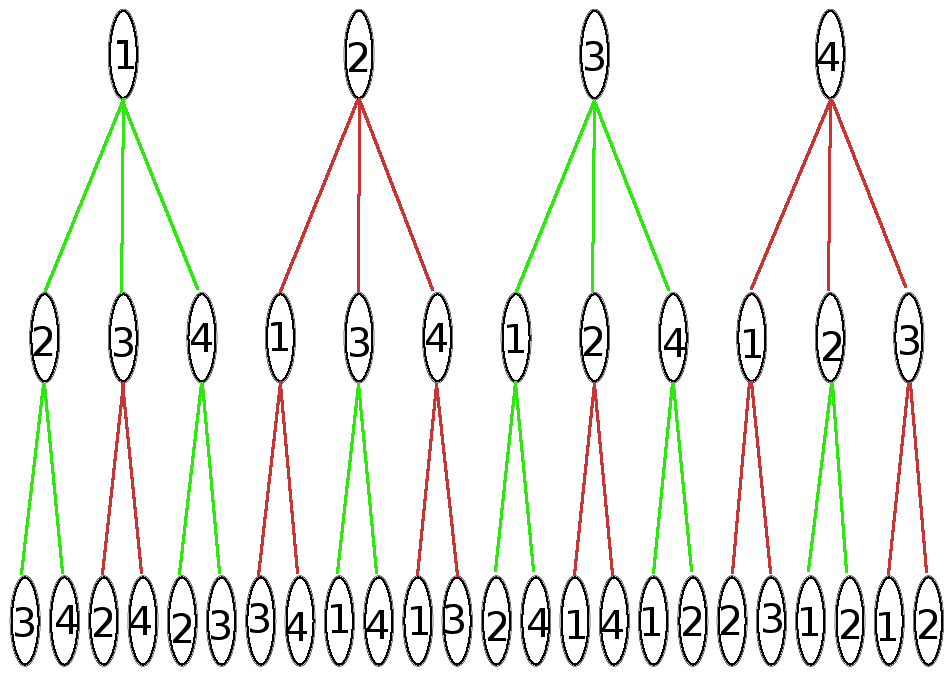
\includegraphics[width=11cm,height=6cm]{img/binomialTree}
  
\end{frame}



\section{Examples}

\begin{frame}
  \frametitle{Example}

  It is estimated that in a given monthly period 55\% od all stocks
  will rise. I pick four stocks at random (with replacement). What is
  the probability that I get exactly one stock that rises?

  \vfill

\end{frame}


\begin{frame}
  \frametitle{Example}

  It is estimated that 2\% of the shirts made at a factory are not
  suitable for sale. You choose 20 shirts at random (with
  replacement). What is the probability that you find exactly three
  unsuitable shirts?

  \vfill

\end{frame}

\begin{frame}{Clicker Quiz}

  A basketball player has a lifetime average of making 60\% of his
  free throws. In a particular game he will attempt ten free
  throws. What is the probability that he will make exactly six free
  throws?

    \vfill

  \begin{tabular}{l@{\hspace{3em}}l@{\hspace{3em}}l@{\hspace{3em}}l}
    A: .20 & B: .25 & C: .50 & D: .60
  \end{tabular}

  \vfill
  \vfill
  \vfill
  
\end{frame}


% LocalWords:  Clarkson pausesection hideallsubsections



\lecture{The Standard Normal Distribution}{standard-normal}
\section{The Standard Normal Distribution}

\title{The Standard Normal Distribution}
\subtitle{A Continuous Random Variable}

\author{Kelly Black}
\institute{Clarkson University}
\date{15 February 2012}

\begin{frame}
  \titlepage
\end{frame}

\begin{frame}
  \frametitle{Outline}
  \tableofcontents[pausesection,hideothersubsections,sectionstyle=show/hide]
\end{frame}


\subsection{The sections}


\begin{frame}
  \frametitle{Clicker Quiz}

  Calculate the value $5 \choose 3 $.
    \vfill

  \begin{tabular}{l@{\hspace{3em}}l@{\hspace{3em}}l}
    A: 20 & B: 15 & C: 10
  \end{tabular}

  \vfill
  \vfill
  \vfill


\end{frame}




\subsection{Another Sections}

\begin{frame}
  \frametitle{}

  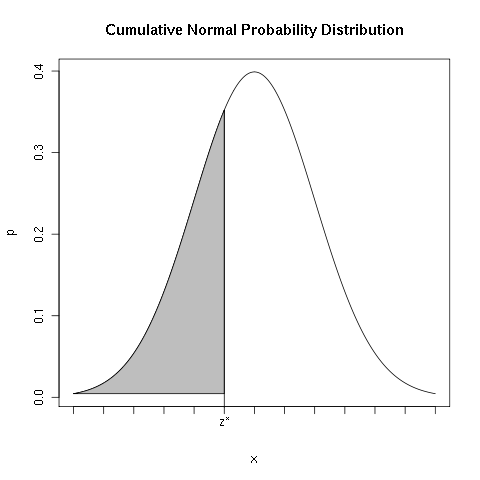
\includegraphics[width=5cm]{img/cummulativeDist}

\end{frame}

\begin{frame}
  \frametitle{The Table}
  \vspace*{-5em}
  \hfill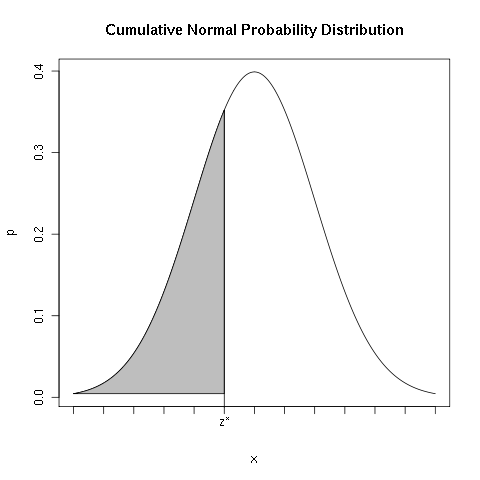
\includegraphics[width=2cm]{img/cummulativeDist}~~~~~~~~~~~~~~

  {
\fontencoding{T1}
\fontfamily{pcr}
\fontseries{m}
\fontshape{n}
\fontsize{5pt}{5pt}
\selectfont

  \begin{tabular}{l|llllllllll}
     & 0.00   & 0.01   & 0.02   & 0.03   &  0.04   & 0.05   & 0.06   & 0.07   & 0.08  & 0.09 \\ \hline
-3.4 & 0.0003 & 0.0003 & 0.0003 & 0.0003 & 0.0003 & 0.0003 & 0.0003 & 0.0003 & 0.0003 & 0.0002 \\ 
-3.3 & 0.0005 & 0.0005 & 0.0005 & 0.0004 & 0.0004 & 0.0004 & 0.0004 & 0.0004 & 0.0004 & 0.0003 \\ 
-3.2 & 0.0007 & 0.0007 & 0.0006 & 0.0006 & 0.0006 & 0.0006 & 0.0006 & 0.0005 & 0.0005 & 0.0005 \\ 
-3.1 & 0.0010 & 0.0009 & 0.0009 & 0.0009 & 0.0008 & 0.0008 & 0.0008 & 0.0008 & 0.0007 & 0.0007 \\ 
-3.0 & 0.0013 & 0.0013 & 0.0013 & 0.0012 & 0.0012 & 0.0011 & 0.0011 & 0.0011 & 0.0010 & 0.0010 \\ 
-2.9 & 0.0019 & 0.0018 & 0.0018 & 0.0017 & 0.0016 & 0.0016 & 0.0015 & 0.0015 & 0.0014 & 0.0014 \\ 
-2.8 & 0.0026 & 0.0025 & 0.0024 & 0.0023 & 0.0023 & 0.0022 & 0.0021 & 0.0021 & 0.0020 & 0.0019 \\ 
-2.7 & 0.0035 & 0.0034 & 0.0033 & 0.0032 & 0.0031 & 0.0030 & 0.0029 & 0.0028 & 0.0027 & 0.0026 \\ 
-2.6 & 0.0047 & 0.0045 & 0.0044 & 0.0043 & 0.0041 & 0.0040 & 0.0039 & 0.0038 & 0.0037 & 0.0036 \\ 
-2.5 & 0.0062 & 0.0060 & 0.0059 & 0.0057 & 0.0055 & 0.0054 & 0.0052 & 0.0051 & 0.0049 & 0.0048 \\ 
-2.4 & 0.0082 & 0.0080 & 0.0078 & 0.0075 & 0.0073 & 0.0071 & 0.0069 & 0.0068 & 0.0066 & 0.0064 \\ 
-2.3 & 0.0107 & 0.0104 & 0.0102 & 0.0099 & 0.0096 & 0.0094 & 0.0091 & 0.0089 & 0.0087 & 0.0084 \\ 
-2.2 & 0.0139 & 0.0136 & 0.0132 & 0.0129 & 0.0125 & 0.0122 & 0.0119 & 0.0116 & 0.0113 & 0.0110 \\ 
-2.1 & 0.0179 & 0.0174 & 0.0170 & 0.0166 & 0.0162 & 0.0158 & 0.0154 & 0.0150 & 0.0146 & 0.0143 \\ 
-2.0 & 0.0228 & 0.0222 & 0.0217 & 0.0212 & 0.0207 & 0.0202 & 0.0197 & 0.0192 & 0.0188 & 0.0183 \\ 
-1.9 & 0.0287 & 0.0281 & 0.0274 & 0.0268 & 0.0262 & 0.0256 & 0.0250 & 0.0244 & 0.0239 & 0.0233 \\ 
-1.8 & 0.0359 & 0.0351 & 0.0344 & 0.0336 & 0.0329 & 0.0322 & 0.0314 & 0.0307 & 0.0301 & 0.0294 \\ 
-1.7 & 0.0446 & 0.0436 & 0.0427 & 0.0418 & 0.0409 & 0.0401 & 0.0392 & 0.0384 & 0.0375 & 0.0367 \\ 
-1.6 & 0.0548 & 0.0537 & 0.0526 & 0.0516 & 0.0505 & 0.0495 & 0.0485 & 0.0475 & 0.0465 & 0.0455 \\ 
-1.5 & 0.0668 & 0.0655 & 0.0643 & 0.0630 & 0.0618 & 0.0606 & 0.0594 & 0.0582 & 0.0571 & 0.0559 \\ 
-1.4 & 0.0808 & 0.0793 & 0.0778 & 0.0764 & 0.0749 & 0.0735 & 0.0721 & 0.0708 & 0.0694 & 0.0681 \\ 
-1.3 & 0.0968 & 0.0951 & 0.0934 & 0.0918 & 0.0901 & 0.0885 & 0.0869 & 0.0853 & 0.0838 & 0.0823 \\ 
-1.2 & 0.1151 & 0.1131 & 0.1112 & 0.1093 & 0.1075 & 0.1056 & 0.1038 & 0.1020 & 0.1003 & 0.0985 \\ 
-1.1 & 0.1357 & 0.1335 & 0.1314 & 0.1292 & 0.1271 & 0.1251 & 0.1230 & 0.1210 & 0.1190 & 0.1170 \\ 
-1.0 & 0.1587 & 0.1562 & 0.1539 & 0.1515 & 0.1492 & 0.1469 & 0.1446 & 0.1423 & 0.1401 & 0.1379 \\ 
-0.9 & 0.1841 & 0.1814 & 0.1788 & 0.1762 & 0.1736 & 0.1711 & 0.1685 & 0.1660 & 0.1635 & 0.1611 \\ 
-0.8 & 0.2119 & 0.2090 & 0.2061 & 0.2033 & 0.2005 & 0.1977 & 0.1949 & 0.1922 & 0.1894 & 0.1867 \\ 
-0.7 & 0.2420 & 0.2389 & 0.2358 & 0.2327 & 0.2296 & 0.2266 & 0.2236 & 0.2206 & 0.2177 & 0.2148 \\ 
-0.6 & 0.2743 & 0.2709 & 0.2676 & 0.2643 & 0.2611 & 0.2578 & 0.2546 & 0.2514 & 0.2483 & 0.2451 \\ 
-0.5 & 0.3085 & 0.3050 & 0.3015 & 0.2981 & 0.2946 & 0.2912 & 0.2877 & 0.2843 & 0.2810 & 0.2776 \\ 
-0.4 & 0.3446 & 0.3409 & 0.3372 & 0.3336 & 0.3300 & 0.3264 & 0.3228 & 0.3192 & 0.3156 & 0.3121 \\ 
-0.3 & 0.3821 & 0.3783 & 0.3745 & 0.3707 & 0.3669 & 0.3632 & 0.3594 & 0.3557 & 0.3520 & 0.3483 \\ 
-0.2 & 0.4207 & 0.4168 & 0.4129 & 0.4090 & 0.4052 & 0.4013 & 0.3974 & 0.3936 & 0.3897 & 0.3859 \\ 
-0.1 & 0.4602 & 0.4562 & 0.4522 & 0.4483 & 0.4443 & 0.4404 & 0.4364 & 0.4325 & 0.4286 & 0.4247 \\ 
-0.0 & 0.5000 & 0.4960 & 0.4920 & 0.4880 & 0.4840 & 0.4801 & 0.4761 & 0.4721 & 0.4681 & 0.4641 
\end{tabular}
}
\end{frame}

\begin{frame}
  \vspace*{-5em}
  \frametitle{The Table}
  \hfill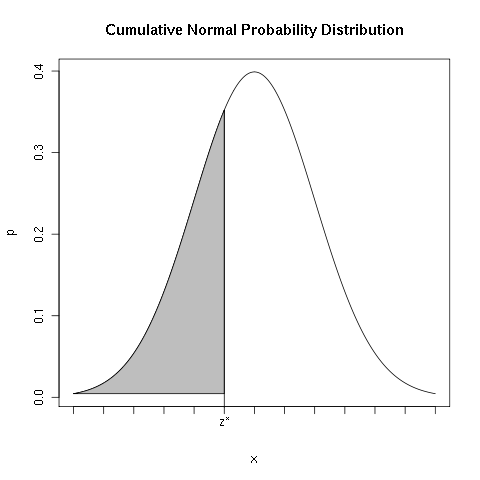
\includegraphics[width=2cm]{img/cummulativeDist}~~~~~~~~~~~~~~

  {
\fontencoding{T1}
\fontfamily{pcr}
\fontseries{m}
\fontshape{n}
\fontsize{5pt}{5pt}
\selectfont
\begin{tabular}{l|llllllllll}
     & 0.00   & 0.01   & 0.02   & 0.03   & 0.04   & 0.05   & 0.06   & 0.07   & 0.08  & 0.09 \\ \hline
0.0 & 0.5000 & 0.5040 & 0.5080 & 0.5120 & 0.5160 & 0.5199 & 0.5239 & 0.5279 & 0.5319 & 0.5359 \\ 
0.1 & 0.5398 & 0.5438 & 0.5478 & 0.5517 & 0.5557 & 0.5596 & 0.5636 & 0.5675 & 0.5714 & 0.5753 \\ 
0.2 & 0.5793 & 0.5832 & 0.5871 & 0.5910 & 0.5948 & 0.5987 & 0.6026 & 0.6064 & 0.6103 & 0.6141 \\ 
0.3 & 0.6179 & 0.6217 & 0.6255 & 0.6293 & 0.6331 & 0.6368 & 0.6406 & 0.6443 & 0.6480 & 0.6517 \\ 
0.4 & 0.6554 & 0.6591 & 0.6628 & 0.6664 & 0.6700 & 0.6736 & 0.6772 & 0.6808 & 0.6844 & 0.6879 \\ 
0.5 & 0.6915 & 0.6950 & 0.6985 & 0.7019 & 0.7054 & 0.7088 & 0.7123 & 0.7157 & 0.7190 & 0.7224 \\ 
0.6 & 0.7257 & 0.7291 & 0.7324 & 0.7357 & 0.7389 & 0.7422 & 0.7454 & 0.7486 & 0.7517 & 0.7549 \\ 
0.7 & 0.7580 & 0.7611 & 0.7642 & 0.7673 & 0.7704 & 0.7734 & 0.7764 & 0.7794 & 0.7823 & 0.7852 \\ 
0.8 & 0.7881 & 0.7910 & 0.7939 & 0.7967 & 0.7995 & 0.8023 & 0.8051 & 0.8078 & 0.8106 & 0.8133 \\ 
0.9 & 0.8159 & 0.8186 & 0.8212 & 0.8238 & 0.8264 & 0.8289 & 0.8315 & 0.8340 & 0.8365 & 0.8389 \\ 
1.0 & 0.8413 & 0.8438 & 0.8461 & 0.8485 & 0.8508 & 0.8531 & 0.8554 & 0.8577 & 0.8599 & 0.8621 \\ 
1.1 & 0.8643 & 0.8665 & 0.8686 & 0.8708 & 0.8729 & 0.8749 & 0.8770 & 0.8790 & 0.8810 & 0.8830 \\ 
1.2 & 0.8849 & 0.8869 & 0.8888 & 0.8907 & 0.8925 & 0.8944 & 0.8962 & 0.8980 & 0.8997 & 0.9015 \\ 
1.3 & 0.9032 & 0.9049 & 0.9066 & 0.9082 & 0.9099 & 0.9115 & 0.9131 & 0.9147 & 0.9162 & 0.9177 \\ 
1.4 & 0.9192 & 0.9207 & 0.9222 & 0.9236 & 0.9251 & 0.9265 & 0.9279 & 0.9292 & 0.9306 & 0.9319 \\ 
1.5 & 0.9332 & 0.9345 & 0.9357 & 0.9370 & 0.9382 & 0.9394 & 0.9406 & 0.9418 & 0.9429 & 0.9441 \\ 
1.6 & 0.9452 & 0.9463 & 0.9474 & 0.9484 & 0.9495 & 0.9505 & 0.9515 & 0.9525 & 0.9535 & 0.9545 \\ 
1.7 & 0.9554 & 0.9564 & 0.9573 & 0.9582 & 0.9591 & 0.9599 & 0.9608 & 0.9616 & 0.9625 & 0.9633 \\ 
1.8 & 0.9641 & 0.9649 & 0.9656 & 0.9664 & 0.9671 & 0.9678 & 0.9686 & 0.9693 & 0.9699 & 0.9706 \\ 
1.9 & 0.9713 & 0.9719 & 0.9726 & 0.9732 & 0.9738 & 0.9744 & 0.9750 & 0.9756 & 0.9761 & 0.9767 \\ 
2.0 & 0.9772 & 0.9778 & 0.9783 & 0.9788 & 0.9793 & 0.9798 & 0.9803 & 0.9808 & 0.9812 & 0.9817 \\ 
2.1 & 0.9821 & 0.9826 & 0.9830 & 0.9834 & 0.9838 & 0.9842 & 0.9846 & 0.9850 & 0.9854 & 0.9857 \\ 
2.2 & 0.9861 & 0.9864 & 0.9868 & 0.9871 & 0.9875 & 0.9878 & 0.9881 & 0.9884 & 0.9887 & 0.9890 \\ 
2.3 & 0.9893 & 0.9896 & 0.9898 & 0.9901 & 0.9904 & 0.9906 & 0.9909 & 0.9911 & 0.9913 & 0.9916 \\ 
2.4 & 0.9918 & 0.9920 & 0.9922 & 0.9925 & 0.9927 & 0.9929 & 0.9931 & 0.9932 & 0.9934 & 0.9936 \\ 
2.5 & 0.9938 & 0.9940 & 0.9941 & 0.9943 & 0.9945 & 0.9946 & 0.9948 & 0.9949 & 0.9951 & 0.9952 \\ 
2.6 & 0.9953 & 0.9955 & 0.9956 & 0.9957 & 0.9959 & 0.9960 & 0.9961 & 0.9962 & 0.9963 & 0.9964 \\ 
2.7 & 0.9965 & 0.9966 & 0.9967 & 0.9968 & 0.9969 & 0.9970 & 0.9971 & 0.9972 & 0.9973 & 0.9974 \\ 
2.8 & 0.9974 & 0.9975 & 0.9976 & 0.9977 & 0.9977 & 0.9978 & 0.9979 & 0.9979 & 0.9980 & 0.9981 \\ 
2.9 & 0.9981 & 0.9982 & 0.9982 & 0.9983 & 0.9984 & 0.9984 & 0.9985 & 0.9985 & 0.9986 & 0.9986 \\ 
3.0 & 0.9987 & 0.9987 & 0.9987 & 0.9988 & 0.9988 & 0.9989 & 0.9989 & 0.9989 & 0.9990 & 0.9990 \\ 
3.1 & 0.9990 & 0.9991 & 0.9991 & 0.9991 & 0.9992 & 0.9992 & 0.9992 & 0.9992 & 0.9993 & 0.9993 \\ 
3.2 & 0.9993 & 0.9993 & 0.9994 & 0.9994 & 0.9994 & 0.9994 & 0.9994 & 0.9995 & 0.9995 & 0.9995 \\ 
3.3 & 0.9995 & 0.9995 & 0.9995 & 0.9996 & 0.9996 & 0.9996 & 0.9996 & 0.9996 & 0.9996 & 0.9997 \\ 
3.4 & 0.9997 & 0.9997 & 0.9997 & 0.9997 & 0.9997 & 0.9997 & 0.9997 & 0.9997 & 0.9997 & 0.9998 
\end{tabular}

}

\end{frame}


\begin{frame}{\small Find the probability that a standard normal is less than -1.75.}
  
{\small First find the row corresponding to -1.7.}

  {
\fontencoding{T1}
\fontfamily{pcr}
\fontseries{m}
\fontshape{n}
\fontsize{5pt}{5pt}
\selectfont

\begin{tabular}{l|llllllllll}
     & 0.00   & 0.01   & 0.02   & 0.03   &  0.04   & 0.05   & 0.06   & 0.07   & 0.08  & 0.09 \\ \hline
-3.4 & 0.0003 & 0.0003 & 0.0003 & 0.0003 & 0.0003 & 0.0003 & 0.0003 & 0.0003 & 0.0003 & 0.0002 \\ 
-3.3 & 0.0005 & 0.0005 & 0.0005 & 0.0004 & 0.0004 & 0.0004 & 0.0004 & 0.0004 & 0.0004 & 0.0003 \\ 
-3.2 & 0.0007 & 0.0007 & 0.0006 & 0.0006 & 0.0006 & 0.0006 & 0.0006 & 0.0005 & 0.0005 & 0.0005 \\ 
-3.1 & 0.0010 & 0.0009 & 0.0009 & 0.0009 & 0.0008 & 0.0008 & 0.0008 & 0.0008 & 0.0007 & 0.0007 \\ 
-3.0 & 0.0013 & 0.0013 & 0.0013 & 0.0012 & 0.0012 & 0.0011 & 0.0011 & 0.0011 & 0.0010 & 0.0010 \\ 
-2.9 & 0.0019 & 0.0018 & 0.0018 & 0.0017 & 0.0016 & 0.0016 & 0.0015 & 0.0015 & 0.0014 & 0.0014 \\ 
-2.8 & 0.0026 & 0.0025 & 0.0024 & 0.0023 & 0.0023 & 0.0022 & 0.0021 & 0.0021 & 0.0020 & 0.0019 \\ 
-2.7 & 0.0035 & 0.0034 & 0.0033 & 0.0032 & 0.0031 & 0.0030 & 0.0029 & 0.0028 & 0.0027 & 0.0026 \\ 
-2.6 & 0.0047 & 0.0045 & 0.0044 & 0.0043 & 0.0041 & 0.0040 & 0.0039 & 0.0038 & 0.0037 & 0.0036 \\ 
-2.5 & 0.0062 & 0.0060 & 0.0059 & 0.0057 & 0.0055 & 0.0054 & 0.0052 & 0.0051 & 0.0049 & 0.0048 \\ 
-2.4 & 0.0082 & 0.0080 & 0.0078 & 0.0075 & 0.0073 & 0.0071 & 0.0069 & 0.0068 & 0.0066 & 0.0064 \\ 
-2.3 & 0.0107 & 0.0104 & 0.0102 & 0.0099 & 0.0096 & 0.0094 & 0.0091 & 0.0089 & 0.0087 & 0.0084 \\ 
-2.2 & 0.0139 & 0.0136 & 0.0132 & 0.0129 & 0.0125 & 0.0122 & 0.0119 & 0.0116 & 0.0113 & 0.0110 \\ 
-2.1 & 0.0179 & 0.0174 & 0.0170 & 0.0166 & 0.0162 & 0.0158 & 0.0154 & 0.0150 & 0.0146 & 0.0143 \\ 
-2.0 & 0.0228 & 0.0222 & 0.0217 & 0.0212 & 0.0207 & 0.0202 & 0.0197 & 0.0192 & 0.0188 & 0.0183 \\ 
-1.9 & 0.0287 & 0.0281 & 0.0274 & 0.0268 & 0.0262 & 0.0256 & 0.0250 & 0.0244 & 0.0239 & 0.0233 \\ 
-1.8 & 0.0359 & 0.0351 & 0.0344 & 0.0336 & 0.0329 & 0.0322 & 0.0314 & 0.0307 & 0.0301 & 0.0294 \\ 
\rowcolor{red} -1.7 & 0.0446 & 0.0436 & 0.0427 & 0.0418 & 0.0409 & 0.0401 & 0.0392 & 0.0384 & 0.0375 & 0.0367 \\ 
-1.6 & 0.0548 & 0.0537 & 0.0526 & 0.0516 & 0.0505 & 0.0495 & 0.0485 & 0.0475 & 0.0465 & 0.0455 \\ 
-1.5 & 0.0668 & 0.0655 & 0.0643 & 0.0630 & 0.0618 & 0.0606 & 0.0594 & 0.0582 & 0.0571 & 0.0559 \\ 
-1.4 & 0.0808 & 0.0793 & 0.0778 & 0.0764 & 0.0749 & 0.0735 & 0.0721 & 0.0708 & 0.0694 & 0.0681 \\ 
-1.3 & 0.0968 & 0.0951 & 0.0934 & 0.0918 & 0.0901 & 0.0885 & 0.0869 & 0.0853 & 0.0838 & 0.0823 \\ 
-1.2 & 0.1151 & 0.1131 & 0.1112 & 0.1093 & 0.1075 & 0.1056 & 0.1038 & 0.1020 & 0.1003 & 0.0985 \\ 
-1.1 & 0.1357 & 0.1335 & 0.1314 & 0.1292 & 0.1271 & 0.1251 & 0.1230 & 0.1210 & 0.1190 & 0.1170 \\ 
-1.0 & 0.1587 & 0.1562 & 0.1539 & 0.1515 & 0.1492 & 0.1469 & 0.1446 & 0.1423 & 0.1401 & 0.1379 \\ 
-0.9 & 0.1841 & 0.1814 & 0.1788 & 0.1762 & 0.1736 & 0.1711 & 0.1685 & 0.1660 & 0.1635 & 0.1611 \\ 
-0.8 & 0.2119 & 0.2090 & 0.2061 & 0.2033 & 0.2005 & 0.1977 & 0.1949 & 0.1922 & 0.1894 & 0.1867 \\ 
-0.7 & 0.2420 & 0.2389 & 0.2358 & 0.2327 & 0.2296 & 0.2266 & 0.2236 & 0.2206 & 0.2177 & 0.2148 \\ 
-0.6 & 0.2743 & 0.2709 & 0.2676 & 0.2643 & 0.2611 & 0.2578 & 0.2546 & 0.2514 & 0.2483 & 0.2451 \\ 
-0.5 & 0.3085 & 0.3050 & 0.3015 & 0.2981 & 0.2946 & 0.2912 & 0.2877 & 0.2843 & 0.2810 & 0.2776 \\ 
-0.4 & 0.3446 & 0.3409 & 0.3372 & 0.3336 & 0.3300 & 0.3264 & 0.3228 & 0.3192 & 0.3156 & 0.3121 \\ 
-0.3 & 0.3821 & 0.3783 & 0.3745 & 0.3707 & 0.3669 & 0.3632 & 0.3594 & 0.3557 & 0.3520 & 0.3483 \\ 
-0.2 & 0.4207 & 0.4168 & 0.4129 & 0.4090 & 0.4052 & 0.4013 & 0.3974 & 0.3936 & 0.3897 & 0.3859 \\ 
-0.1 & 0.4602 & 0.4562 & 0.4522 & 0.4483 & 0.4443 & 0.4404 & 0.4364 & 0.4325 & 0.4286 & 0.4247 \\ 
-0.0 & 0.5000 & 0.4960 & 0.4920 & 0.4880 & 0.4840 & 0.4801 & 0.4761 & 0.4721 & 0.4681 & 0.4641 
\end{tabular}


}


\end{frame}

\begin{frame} {\small First find the row corresponding to -1.7. Second
    find the column corresponding to 0.05. The probability is the
    intersection of the row and column, 0.0401.}

  {
\fontencoding{T1}
\fontfamily{pcr}
\fontseries{m}
\fontshape{n}
\fontsize{5pt}{5pt}
\selectfont

\begin{tabular}{l|lllll>{\columncolor{blue}}lllll}
     & 0.00   & 0.01   & 0.02   & 0.03   &  0.04   & 0.05   & 0.06   & 0.07   & 0.08  & 0.09 \\ \hline
-3.4 & 0.0003 & 0.0003 & 0.0003 & 0.0003 & 0.0003 & 0.0003 & 0.0003 & 0.0003 & 0.0003 & 0.0002 \\ 
-3.3 & 0.0005 & 0.0005 & 0.0005 & 0.0004 & 0.0004 & 0.0004 & 0.0004 & 0.0004 & 0.0004 & 0.0003 \\ 
-3.2 & 0.0007 & 0.0007 & 0.0006 & 0.0006 & 0.0006 & 0.0006 & 0.0006 & 0.0005 & 0.0005 & 0.0005 \\ 
-3.1 & 0.0010 & 0.0009 & 0.0009 & 0.0009 & 0.0008 & 0.0008 & 0.0008 & 0.0008 & 0.0007 & 0.0007 \\ 
-3.0 & 0.0013 & 0.0013 & 0.0013 & 0.0012 & 0.0012 & 0.0011 & 0.0011 & 0.0011 & 0.0010 & 0.0010 \\ 
-2.9 & 0.0019 & 0.0018 & 0.0018 & 0.0017 & 0.0016 & 0.0016 & 0.0015 & 0.0015 & 0.0014 & 0.0014 \\ 
-2.8 & 0.0026 & 0.0025 & 0.0024 & 0.0023 & 0.0023 & 0.0022 & 0.0021 & 0.0021 & 0.0020 & 0.0019 \\ 
-2.7 & 0.0035 & 0.0034 & 0.0033 & 0.0032 & 0.0031 & 0.0030 & 0.0029 & 0.0028 & 0.0027 & 0.0026 \\ 
-2.6 & 0.0047 & 0.0045 & 0.0044 & 0.0043 & 0.0041 & 0.0040 & 0.0039 & 0.0038 & 0.0037 & 0.0036 \\ 
-2.5 & 0.0062 & 0.0060 & 0.0059 & 0.0057 & 0.0055 & 0.0054 & 0.0052 & 0.0051 & 0.0049 & 0.0048 \\ 
-2.4 & 0.0082 & 0.0080 & 0.0078 & 0.0075 & 0.0073 & 0.0071 & 0.0069 & 0.0068 & 0.0066 & 0.0064 \\ 
-2.3 & 0.0107 & 0.0104 & 0.0102 & 0.0099 & 0.0096 & 0.0094 & 0.0091 & 0.0089 & 0.0087 & 0.0084 \\ 
-2.2 & 0.0139 & 0.0136 & 0.0132 & 0.0129 & 0.0125 & 0.0122 & 0.0119 & 0.0116 & 0.0113 & 0.0110 \\ 
-2.1 & 0.0179 & 0.0174 & 0.0170 & 0.0166 & 0.0162 & 0.0158 & 0.0154 & 0.0150 & 0.0146 & 0.0143 \\ 
-2.0 & 0.0228 & 0.0222 & 0.0217 & 0.0212 & 0.0207 & 0.0202 & 0.0197 & 0.0192 & 0.0188 & 0.0183 \\ 
-1.9 & 0.0287 & 0.0281 & 0.0274 & 0.0268 & 0.0262 & 0.0256 & 0.0250 & 0.0244 & 0.0239 & 0.0233 \\ 
-1.8 & 0.0359 & 0.0351 & 0.0344 & 0.0336 & 0.0329 & 0.0322 & 0.0314 & 0.0307 & 0.0301 & 0.0294 \\ 
\rowcolor{red} -1.7 & 0.0446 & 0.0436 & 0.0427 & 0.0418 & 0.0409 & {\colorbox{yellow}{~~0.0401}~~} & 0.0392 & 0.0384 & 0.0375 & 0.0367 \\ 
-1.6 & 0.0548 & 0.0537 & 0.0526 & 0.0516 & 0.0505 & 0.0495 & 0.0485 & 0.0475 & 0.0465 & 0.0455 \\ 
-1.5 & 0.0668 & 0.0655 & 0.0643 & 0.0630 & 0.0618 & 0.0606 & 0.0594 & 0.0582 & 0.0571 & 0.0559 \\ 
-1.4 & 0.0808 & 0.0793 & 0.0778 & 0.0764 & 0.0749 & 0.0735 & 0.0721 & 0.0708 & 0.0694 & 0.0681 \\ 
-1.3 & 0.0968 & 0.0951 & 0.0934 & 0.0918 & 0.0901 & 0.0885 & 0.0869 & 0.0853 & 0.0838 & 0.0823 \\ 
-1.2 & 0.1151 & 0.1131 & 0.1112 & 0.1093 & 0.1075 & 0.1056 & 0.1038 & 0.1020 & 0.1003 & 0.0985 \\ 
-1.1 & 0.1357 & 0.1335 & 0.1314 & 0.1292 & 0.1271 & 0.1251 & 0.1230 & 0.1210 & 0.1190 & 0.1170 \\ 
-1.0 & 0.1587 & 0.1562 & 0.1539 & 0.1515 & 0.1492 & 0.1469 & 0.1446 & 0.1423 & 0.1401 & 0.1379 \\ 
-0.9 & 0.1841 & 0.1814 & 0.1788 & 0.1762 & 0.1736 & 0.1711 & 0.1685 & 0.1660 & 0.1635 & 0.1611 \\ 
-0.8 & 0.2119 & 0.2090 & 0.2061 & 0.2033 & 0.2005 & 0.1977 & 0.1949 & 0.1922 & 0.1894 & 0.1867 \\ 
-0.7 & 0.2420 & 0.2389 & 0.2358 & 0.2327 & 0.2296 & 0.2266 & 0.2236 & 0.2206 & 0.2177 & 0.2148 \\ 
-0.6 & 0.2743 & 0.2709 & 0.2676 & 0.2643 & 0.2611 & 0.2578 & 0.2546 & 0.2514 & 0.2483 & 0.2451 \\ 
-0.5 & 0.3085 & 0.3050 & 0.3015 & 0.2981 & 0.2946 & 0.2912 & 0.2877 & 0.2843 & 0.2810 & 0.2776 \\ 
-0.4 & 0.3446 & 0.3409 & 0.3372 & 0.3336 & 0.3300 & 0.3264 & 0.3228 & 0.3192 & 0.3156 & 0.3121 \\ 
-0.3 & 0.3821 & 0.3783 & 0.3745 & 0.3707 & 0.3669 & 0.3632 & 0.3594 & 0.3557 & 0.3520 & 0.3483 \\ 
-0.2 & 0.4207 & 0.4168 & 0.4129 & 0.4090 & 0.4052 & 0.4013 & 0.3974 & 0.3936 & 0.3897 & 0.3859 \\ 
-0.1 & 0.4602 & 0.4562 & 0.4522 & 0.4483 & 0.4443 & 0.4404 & 0.4364 & 0.4325 & 0.4286 & 0.4247 \\ 
-0.0 & 0.5000 & 0.4960 & 0.4920 & 0.4880 & 0.4840 & 0.4801 & 0.4761 & 0.4721 & 0.4681 & 0.4641 
\end{tabular}



}

\end{frame}




\begin{frame}{\small Find the probability that a standard normal is less than 0.87.}
  
{\small First find the row corresponding to 0.8.}

  {
\fontencoding{T1}
\fontfamily{pcr}
\fontseries{m}
\fontshape{n}
\fontsize{5pt}{5pt}
\selectfont

\begin{tabular}{l|llllllllll}
     & 0.00   & 0.01   & 0.02   & 0.03   & 0.04   & 0.05   & 0.06   & 0.07   & 0.08  & 0.09 \\ \hline
0.0 & 0.5000 & 0.5040 & 0.5080 & 0.5120 & 0.5160 & 0.5199 & 0.5239 & 0.5279 & 0.5319 & 0.5359 \\ 
0.1 & 0.5398 & 0.5438 & 0.5478 & 0.5517 & 0.5557 & 0.5596 & 0.5636 & 0.5675 & 0.5714 & 0.5753 \\ 
0.2 & 0.5793 & 0.5832 & 0.5871 & 0.5910 & 0.5948 & 0.5987 & 0.6026 & 0.6064 & 0.6103 & 0.6141 \\ 
0.3 & 0.6179 & 0.6217 & 0.6255 & 0.6293 & 0.6331 & 0.6368 & 0.6406 & 0.6443 & 0.6480 & 0.6517 \\ 
0.4 & 0.6554 & 0.6591 & 0.6628 & 0.6664 & 0.6700 & 0.6736 & 0.6772 & 0.6808 & 0.6844 & 0.6879 \\ 
0.5 & 0.6915 & 0.6950 & 0.6985 & 0.7019 & 0.7054 & 0.7088 & 0.7123 & 0.7157 & 0.7190 & 0.7224 \\ 
0.6 & 0.7257 & 0.7291 & 0.7324 & 0.7357 & 0.7389 & 0.7422 & 0.7454 & 0.7486 & 0.7517 & 0.7549 \\ 
0.7 & 0.7580 & 0.7611 & 0.7642 & 0.7673 & 0.7704 & 0.7734 & 0.7764 & 0.7794 & 0.7823 & 0.7852 \\ 
\rowcolor{red}0.8 & 0.7881 & 0.7910 & 0.7939 & 0.7967 & 0.7995 & 0.8023 & 0.8051 & 0.8078 & 0.8106 & 0.8133 \\ 
0.9 & 0.8159 & 0.8186 & 0.8212 & 0.8238 & 0.8264 & 0.8289 & 0.8315 & 0.8340 & 0.8365 & 0.8389 \\ 
1.0 & 0.8413 & 0.8438 & 0.8461 & 0.8485 & 0.8508 & 0.8531 & 0.8554 & 0.8577 & 0.8599 & 0.8621 \\ 
1.1 & 0.8643 & 0.8665 & 0.8686 & 0.8708 & 0.8729 & 0.8749 & 0.8770 & 0.8790 & 0.8810 & 0.8830 \\ 
1.2 & 0.8849 & 0.8869 & 0.8888 & 0.8907 & 0.8925 & 0.8944 & 0.8962 & 0.8980 & 0.8997 & 0.9015 \\ 
1.3 & 0.9032 & 0.9049 & 0.9066 & 0.9082 & 0.9099 & 0.9115 & 0.9131 & 0.9147 & 0.9162 & 0.9177 \\ 
1.4 & 0.9192 & 0.9207 & 0.9222 & 0.9236 & 0.9251 & 0.9265 & 0.9279 & 0.9292 & 0.9306 & 0.9319 \\ 
1.5 & 0.9332 & 0.9345 & 0.9357 & 0.9370 & 0.9382 & 0.9394 & 0.9406 & 0.9418 & 0.9429 & 0.9441 \\ 
1.6 & 0.9452 & 0.9463 & 0.9474 & 0.9484 & 0.9495 & 0.9505 & 0.9515 & 0.9525 & 0.9535 & 0.9545 \\ 
1.7 & 0.9554 & 0.9564 & 0.9573 & 0.9582 & 0.9591 & 0.9599 & 0.9608 & 0.9616 & 0.9625 & 0.9633 \\ 
1.8 & 0.9641 & 0.9649 & 0.9656 & 0.9664 & 0.9671 & 0.9678 & 0.9686 & 0.9693 & 0.9699 & 0.9706 \\ 
1.9 & 0.9713 & 0.9719 & 0.9726 & 0.9732 & 0.9738 & 0.9744 & 0.9750 & 0.9756 & 0.9761 & 0.9767 \\ 
2.0 & 0.9772 & 0.9778 & 0.9783 & 0.9788 & 0.9793 & 0.9798 & 0.9803 & 0.9808 & 0.9812 & 0.9817 \\ 
2.1 & 0.9821 & 0.9826 & 0.9830 & 0.9834 & 0.9838 & 0.9842 & 0.9846 & 0.9850 & 0.9854 & 0.9857 \\ 
2.2 & 0.9861 & 0.9864 & 0.9868 & 0.9871 & 0.9875 & 0.9878 & 0.9881 & 0.9884 & 0.9887 & 0.9890 \\ 
2.3 & 0.9893 & 0.9896 & 0.9898 & 0.9901 & 0.9904 & 0.9906 & 0.9909 & 0.9911 & 0.9913 & 0.9916 \\ 
2.4 & 0.9918 & 0.9920 & 0.9922 & 0.9925 & 0.9927 & 0.9929 & 0.9931 & 0.9932 & 0.9934 & 0.9936 \\ 
2.5 & 0.9938 & 0.9940 & 0.9941 & 0.9943 & 0.9945 & 0.9946 & 0.9948 & 0.9949 & 0.9951 & 0.9952 \\ 
2.6 & 0.9953 & 0.9955 & 0.9956 & 0.9957 & 0.9959 & 0.9960 & 0.9961 & 0.9962 & 0.9963 & 0.9964 \\ 
2.7 & 0.9965 & 0.9966 & 0.9967 & 0.9968 & 0.9969 & 0.9970 & 0.9971 & 0.9972 & 0.9973 & 0.9974 \\ 
2.8 & 0.9974 & 0.9975 & 0.9976 & 0.9977 & 0.9977 & 0.9978 & 0.9979 & 0.9979 & 0.9980 & 0.9981 \\ 
2.9 & 0.9981 & 0.9982 & 0.9982 & 0.9983 & 0.9984 & 0.9984 & 0.9985 & 0.9985 & 0.9986 & 0.9986 \\ 
3.0 & 0.9987 & 0.9987 & 0.9987 & 0.9988 & 0.9988 & 0.9989 & 0.9989 & 0.9989 & 0.9990 & 0.9990 \\ 
3.1 & 0.9990 & 0.9991 & 0.9991 & 0.9991 & 0.9992 & 0.9992 & 0.9992 & 0.9992 & 0.9993 & 0.9993 \\ 
3.2 & 0.9993 & 0.9993 & 0.9994 & 0.9994 & 0.9994 & 0.9994 & 0.9994 & 0.9995 & 0.9995 & 0.9995 \\ 
3.3 & 0.9995 & 0.9995 & 0.9995 & 0.9996 & 0.9996 & 0.9996 & 0.9996 & 0.9996 & 0.9996 & 0.9997 \\ 
3.4 & 0.9997 & 0.9997 & 0.9997 & 0.9997 & 0.9997 & 0.9997 & 0.9997 & 0.9997 & 0.9997 & 0.9998 
\end{tabular}


}


\end{frame}

\begin{frame}
{\small Second find the column corresponding to 0.07. The probability is the
intersection of the row and column, 0.8078.}

  {
\fontencoding{T1}
\fontfamily{pcr}
\fontseries{m}
\fontshape{n}
\fontsize{5pt}{5pt}
\selectfont

\begin{tabular}{l|lllllll>{\columncolor{blue}}lll}
     & 0.00   & 0.01   & 0.02   & 0.03   & 0.04   & 0.05   & 0.06   & 0.07   & 0.08  & 0.09 \\ \hline
0.0 & 0.5000 & 0.5040 & 0.5080 & 0.5120 & 0.5160 & 0.5199 & 0.5239 & 0.5279 & 0.5319 & 0.5359 \\ 
0.1 & 0.5398 & 0.5438 & 0.5478 & 0.5517 & 0.5557 & 0.5596 & 0.5636 & 0.5675 & 0.5714 & 0.5753 \\ 
0.2 & 0.5793 & 0.5832 & 0.5871 & 0.5910 & 0.5948 & 0.5987 & 0.6026 & 0.6064 & 0.6103 & 0.6141 \\ 
0.3 & 0.6179 & 0.6217 & 0.6255 & 0.6293 & 0.6331 & 0.6368 & 0.6406 & 0.6443 & 0.6480 & 0.6517 \\ 
0.4 & 0.6554 & 0.6591 & 0.6628 & 0.6664 & 0.6700 & 0.6736 & 0.6772 & 0.6808 & 0.6844 & 0.6879 \\ 
0.5 & 0.6915 & 0.6950 & 0.6985 & 0.7019 & 0.7054 & 0.7088 & 0.7123 & 0.7157 & 0.7190 & 0.7224 \\ 
0.6 & 0.7257 & 0.7291 & 0.7324 & 0.7357 & 0.7389 & 0.7422 & 0.7454 & 0.7486 & 0.7517 & 0.7549 \\ 
0.7 & 0.7580 & 0.7611 & 0.7642 & 0.7673 & 0.7704 & 0.7734 & 0.7764 & 0.7794 & 0.7823 & 0.7852 \\ 
\rowcolor{red}0.8 & 0.7881 & 0.7910 & 0.7939 & 0.7967 & 0.7995 & 0.8023 & 0.8051 & {\colorbox{yellow}{~~0.8078~~}} & 0.8106 & 0.8133 \\ 
0.9 & 0.8159 & 0.8186 & 0.8212 & 0.8238 & 0.8264 & 0.8289 & 0.8315 & 0.8340 & 0.8365 & 0.8389 \\ 
1.0 & 0.8413 & 0.8438 & 0.8461 & 0.8485 & 0.8508 & 0.8531 & 0.8554 & 0.8577 & 0.8599 & 0.8621 \\ 
1.1 & 0.8643 & 0.8665 & 0.8686 & 0.8708 & 0.8729 & 0.8749 & 0.8770 & 0.8790 & 0.8810 & 0.8830 \\ 
1.2 & 0.8849 & 0.8869 & 0.8888 & 0.8907 & 0.8925 & 0.8944 & 0.8962 & 0.8980 & 0.8997 & 0.9015 \\ 
1.3 & 0.9032 & 0.9049 & 0.9066 & 0.9082 & 0.9099 & 0.9115 & 0.9131 & 0.9147 & 0.9162 & 0.9177 \\ 
1.4 & 0.9192 & 0.9207 & 0.9222 & 0.9236 & 0.9251 & 0.9265 & 0.9279 & 0.9292 & 0.9306 & 0.9319 \\ 
1.5 & 0.9332 & 0.9345 & 0.9357 & 0.9370 & 0.9382 & 0.9394 & 0.9406 & 0.9418 & 0.9429 & 0.9441 \\ 
1.6 & 0.9452 & 0.9463 & 0.9474 & 0.9484 & 0.9495 & 0.9505 & 0.9515 & 0.9525 & 0.9535 & 0.9545 \\ 
1.7 & 0.9554 & 0.9564 & 0.9573 & 0.9582 & 0.9591 & 0.9599 & 0.9608 & 0.9616 & 0.9625 & 0.9633 \\ 
1.8 & 0.9641 & 0.9649 & 0.9656 & 0.9664 & 0.9671 & 0.9678 & 0.9686 & 0.9693 & 0.9699 & 0.9706 \\ 
1.9 & 0.9713 & 0.9719 & 0.9726 & 0.9732 & 0.9738 & 0.9744 & 0.9750 & 0.9756 & 0.9761 & 0.9767 \\ 
2.0 & 0.9772 & 0.9778 & 0.9783 & 0.9788 & 0.9793 & 0.9798 & 0.9803 & 0.9808 & 0.9812 & 0.9817 \\ 
2.1 & 0.9821 & 0.9826 & 0.9830 & 0.9834 & 0.9838 & 0.9842 & 0.9846 & 0.9850 & 0.9854 & 0.9857 \\ 
2.2 & 0.9861 & 0.9864 & 0.9868 & 0.9871 & 0.9875 & 0.9878 & 0.9881 & 0.9884 & 0.9887 & 0.9890 \\ 
2.3 & 0.9893 & 0.9896 & 0.9898 & 0.9901 & 0.9904 & 0.9906 & 0.9909 & 0.9911 & 0.9913 & 0.9916 \\ 
2.4 & 0.9918 & 0.9920 & 0.9922 & 0.9925 & 0.9927 & 0.9929 & 0.9931 & 0.9932 & 0.9934 & 0.9936 \\ 
2.5 & 0.9938 & 0.9940 & 0.9941 & 0.9943 & 0.9945 & 0.9946 & 0.9948 & 0.9949 & 0.9951 & 0.9952 \\ 
2.6 & 0.9953 & 0.9955 & 0.9956 & 0.9957 & 0.9959 & 0.9960 & 0.9961 & 0.9962 & 0.9963 & 0.9964 \\ 
2.7 & 0.9965 & 0.9966 & 0.9967 & 0.9968 & 0.9969 & 0.9970 & 0.9971 & 0.9972 & 0.9973 & 0.9974 \\ 
2.8 & 0.9974 & 0.9975 & 0.9976 & 0.9977 & 0.9977 & 0.9978 & 0.9979 & 0.9979 & 0.9980 & 0.9981 \\ 
2.9 & 0.9981 & 0.9982 & 0.9982 & 0.9983 & 0.9984 & 0.9984 & 0.9985 & 0.9985 & 0.9986 & 0.9986 \\ 
3.0 & 0.9987 & 0.9987 & 0.9987 & 0.9988 & 0.9988 & 0.9989 & 0.9989 & 0.9989 & 0.9990 & 0.9990 \\ 
3.1 & 0.9990 & 0.9991 & 0.9991 & 0.9991 & 0.9992 & 0.9992 & 0.9992 & 0.9992 & 0.9993 & 0.9993 \\ 
3.2 & 0.9993 & 0.9993 & 0.9994 & 0.9994 & 0.9994 & 0.9994 & 0.9994 & 0.9995 & 0.9995 & 0.9995 \\ 
3.3 & 0.9995 & 0.9995 & 0.9995 & 0.9996 & 0.9996 & 0.9996 & 0.9996 & 0.9996 & 0.9996 & 0.9997 \\ 
3.4 & 0.9997 & 0.9997 & 0.9997 & 0.9997 & 0.9997 & 0.9997 & 0.9997 & 0.9997 & 0.9997 & 0.9998 
\end{tabular}



}

\end{frame}


\begin{frame}
  \frametitle{Clicker Quiz}

  Find $p(1.46 \leq Z \leq 2.13)$.
  \vfill

  \begin{tabular}{l@{\hspace{3em}}l@{\hspace{3em}}l@{\hspace{3em}}l}
    A: 0.0555 & B: 0.0703  & C: 0.6700 & D: 0.9834
  \end{tabular}
  % .9834-.9279 = 0.0555

  \vfill
  \vfill
  \vfill


\end{frame}


% LocalWords:  Clarkson pausesection hideallsubsections




% %%%%%%%%%%%%%%%%%%%%%%%%%%%%%%%%%%%%%%%%%%%%%%%%%%%%%%%%%%%%


\lecture{Normal Distributions}{normal-distributions-not-standard}
\part{Normal Distributions}

\title{Normal Distributions}
\subtitle{Distributions That Are Not The Standard Normal}

\author{Kelly Black}
\institute{Clarkson University}
\date{February 20 2012}

\begin{frame}
  \titlepage
\end{frame}

\begin{frame}
  \frametitle{Outline}
  \tableofcontents[pausesection,hideallsubsections,part=1]
\end{frame}


\section{Clicker Quiz}


\begin{frame}
  \frametitle{Clicker Quiz}

  What is the probability that a random variable that follows a
  standard normal distribution is less than 1.36?

  \vfill

  \begin{tabular}{l@{\hspace{3em}}l@{\hspace{3em}}l}
    A: .9032 & B: .9131 & C: .9147
  \end{tabular}

  \vfill
  \vfill
  \vfill


\end{frame}


\begin{frame}
  \frametitle{The Table}
  \vspace*{-5em}
  \hfill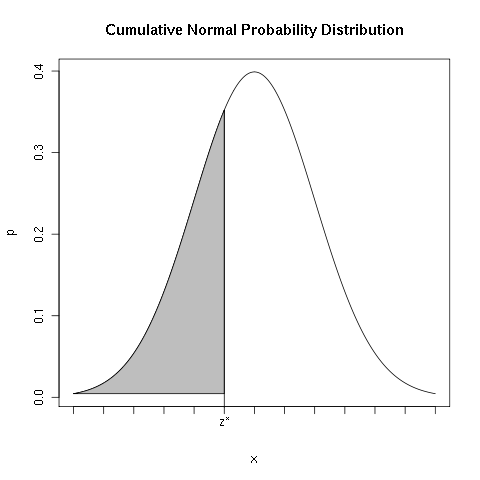
\includegraphics[width=2cm]{img/cummulativeDist}~~~~~~~~~~~~~~

  {
\fontencoding{T1}
\fontfamily{pcr}
\fontseries{m}
\fontshape{n}
\fontsize{5pt}{5pt}
\selectfont

  \begin{tabular}{l|llllllllll}
     & 0.00   & 0.01   & 0.02   & 0.03   &  0.04   & 0.05   & 0.06   & 0.07   & 0.08  & 0.09 \\ \hline
-3.4 & 0.0003 & 0.0003 & 0.0003 & 0.0003 & 0.0003 & 0.0003 & 0.0003 & 0.0003 & 0.0003 & 0.0002 \\ 
-3.3 & 0.0005 & 0.0005 & 0.0005 & 0.0004 & 0.0004 & 0.0004 & 0.0004 & 0.0004 & 0.0004 & 0.0003 \\ 
-3.2 & 0.0007 & 0.0007 & 0.0006 & 0.0006 & 0.0006 & 0.0006 & 0.0006 & 0.0005 & 0.0005 & 0.0005 \\ 
-3.1 & 0.0010 & 0.0009 & 0.0009 & 0.0009 & 0.0008 & 0.0008 & 0.0008 & 0.0008 & 0.0007 & 0.0007 \\ 
-3.0 & 0.0013 & 0.0013 & 0.0013 & 0.0012 & 0.0012 & 0.0011 & 0.0011 & 0.0011 & 0.0010 & 0.0010 \\ 
-2.9 & 0.0019 & 0.0018 & 0.0018 & 0.0017 & 0.0016 & 0.0016 & 0.0015 & 0.0015 & 0.0014 & 0.0014 \\ 
-2.8 & 0.0026 & 0.0025 & 0.0024 & 0.0023 & 0.0023 & 0.0022 & 0.0021 & 0.0021 & 0.0020 & 0.0019 \\ 
-2.7 & 0.0035 & 0.0034 & 0.0033 & 0.0032 & 0.0031 & 0.0030 & 0.0029 & 0.0028 & 0.0027 & 0.0026 \\ 
-2.6 & 0.0047 & 0.0045 & 0.0044 & 0.0043 & 0.0041 & 0.0040 & 0.0039 & 0.0038 & 0.0037 & 0.0036 \\ 
-2.5 & 0.0062 & 0.0060 & 0.0059 & 0.0057 & 0.0055 & 0.0054 & 0.0052 & 0.0051 & 0.0049 & 0.0048 \\ 
-2.4 & 0.0082 & 0.0080 & 0.0078 & 0.0075 & 0.0073 & 0.0071 & 0.0069 & 0.0068 & 0.0066 & 0.0064 \\ 
-2.3 & 0.0107 & 0.0104 & 0.0102 & 0.0099 & 0.0096 & 0.0094 & 0.0091 & 0.0089 & 0.0087 & 0.0084 \\ 
-2.2 & 0.0139 & 0.0136 & 0.0132 & 0.0129 & 0.0125 & 0.0122 & 0.0119 & 0.0116 & 0.0113 & 0.0110 \\ 
-2.1 & 0.0179 & 0.0174 & 0.0170 & 0.0166 & 0.0162 & 0.0158 & 0.0154 & 0.0150 & 0.0146 & 0.0143 \\ 
-2.0 & 0.0228 & 0.0222 & 0.0217 & 0.0212 & 0.0207 & 0.0202 & 0.0197 & 0.0192 & 0.0188 & 0.0183 \\ 
-1.9 & 0.0287 & 0.0281 & 0.0274 & 0.0268 & 0.0262 & 0.0256 & 0.0250 & 0.0244 & 0.0239 & 0.0233 \\ 
-1.8 & 0.0359 & 0.0351 & 0.0344 & 0.0336 & 0.0329 & 0.0322 & 0.0314 & 0.0307 & 0.0301 & 0.0294 \\ 
-1.7 & 0.0446 & 0.0436 & 0.0427 & 0.0418 & 0.0409 & 0.0401 & 0.0392 & 0.0384 & 0.0375 & 0.0367 \\ 
-1.6 & 0.0548 & 0.0537 & 0.0526 & 0.0516 & 0.0505 & 0.0495 & 0.0485 & 0.0475 & 0.0465 & 0.0455 \\ 
-1.5 & 0.0668 & 0.0655 & 0.0643 & 0.0630 & 0.0618 & 0.0606 & 0.0594 & 0.0582 & 0.0571 & 0.0559 \\ 
-1.4 & 0.0808 & 0.0793 & 0.0778 & 0.0764 & 0.0749 & 0.0735 & 0.0721 & 0.0708 & 0.0694 & 0.0681 \\ 
-1.3 & 0.0968 & 0.0951 & 0.0934 & 0.0918 & 0.0901 & 0.0885 & 0.0869 & 0.0853 & 0.0838 & 0.0823 \\ 
-1.2 & 0.1151 & 0.1131 & 0.1112 & 0.1093 & 0.1075 & 0.1056 & 0.1038 & 0.1020 & 0.1003 & 0.0985 \\ 
-1.1 & 0.1357 & 0.1335 & 0.1314 & 0.1292 & 0.1271 & 0.1251 & 0.1230 & 0.1210 & 0.1190 & 0.1170 \\ 
-1.0 & 0.1587 & 0.1562 & 0.1539 & 0.1515 & 0.1492 & 0.1469 & 0.1446 & 0.1423 & 0.1401 & 0.1379 \\ 
-0.9 & 0.1841 & 0.1814 & 0.1788 & 0.1762 & 0.1736 & 0.1711 & 0.1685 & 0.1660 & 0.1635 & 0.1611 \\ 
-0.8 & 0.2119 & 0.2090 & 0.2061 & 0.2033 & 0.2005 & 0.1977 & 0.1949 & 0.1922 & 0.1894 & 0.1867 \\ 
-0.7 & 0.2420 & 0.2389 & 0.2358 & 0.2327 & 0.2296 & 0.2266 & 0.2236 & 0.2206 & 0.2177 & 0.2148 \\ 
-0.6 & 0.2743 & 0.2709 & 0.2676 & 0.2643 & 0.2611 & 0.2578 & 0.2546 & 0.2514 & 0.2483 & 0.2451 \\ 
-0.5 & 0.3085 & 0.3050 & 0.3015 & 0.2981 & 0.2946 & 0.2912 & 0.2877 & 0.2843 & 0.2810 & 0.2776 \\ 
-0.4 & 0.3446 & 0.3409 & 0.3372 & 0.3336 & 0.3300 & 0.3264 & 0.3228 & 0.3192 & 0.3156 & 0.3121 \\ 
-0.3 & 0.3821 & 0.3783 & 0.3745 & 0.3707 & 0.3669 & 0.3632 & 0.3594 & 0.3557 & 0.3520 & 0.3483 \\ 
-0.2 & 0.4207 & 0.4168 & 0.4129 & 0.4090 & 0.4052 & 0.4013 & 0.3974 & 0.3936 & 0.3897 & 0.3859 \\ 
-0.1 & 0.4602 & 0.4562 & 0.4522 & 0.4483 & 0.4443 & 0.4404 & 0.4364 & 0.4325 & 0.4286 & 0.4247 \\ 
-0.0 & 0.5000 & 0.4960 & 0.4920 & 0.4880 & 0.4840 & 0.4801 & 0.4761 & 0.4721 & 0.4681 & 0.4641 
\end{tabular}
}
\end{frame}


\begin{frame}
  \vspace*{-5em}
  \frametitle{The Table}
  \hfill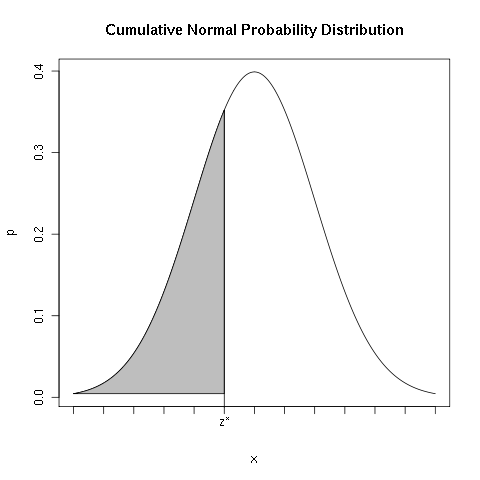
\includegraphics[width=2cm]{img/cummulativeDist}~~~~~~~~~~~~~~

  {
\fontencoding{T1}
\fontfamily{pcr}
\fontseries{m}
\fontshape{n}
\fontsize{5pt}{5pt}
\selectfont
\begin{tabular}{l|llllllllll}
     & 0.00   & 0.01   & 0.02   & 0.03   & 0.04   & 0.05   & 0.06   & 0.07   & 0.08  & 0.09 \\ \hline
0.0 & 0.5000 & 0.5040 & 0.5080 & 0.5120 & 0.5160 & 0.5199 & 0.5239 & 0.5279 & 0.5319 & 0.5359 \\ 
0.1 & 0.5398 & 0.5438 & 0.5478 & 0.5517 & 0.5557 & 0.5596 & 0.5636 & 0.5675 & 0.5714 & 0.5753 \\ 
0.2 & 0.5793 & 0.5832 & 0.5871 & 0.5910 & 0.5948 & 0.5987 & 0.6026 & 0.6064 & 0.6103 & 0.6141 \\ 
0.3 & 0.6179 & 0.6217 & 0.6255 & 0.6293 & 0.6331 & 0.6368 & 0.6406 & 0.6443 & 0.6480 & 0.6517 \\ 
0.4 & 0.6554 & 0.6591 & 0.6628 & 0.6664 & 0.6700 & 0.6736 & 0.6772 & 0.6808 & 0.6844 & 0.6879 \\ 
0.5 & 0.6915 & 0.6950 & 0.6985 & 0.7019 & 0.7054 & 0.7088 & 0.7123 & 0.7157 & 0.7190 & 0.7224 \\ 
0.6 & 0.7257 & 0.7291 & 0.7324 & 0.7357 & 0.7389 & 0.7422 & 0.7454 & 0.7486 & 0.7517 & 0.7549 \\ 
0.7 & 0.7580 & 0.7611 & 0.7642 & 0.7673 & 0.7704 & 0.7734 & 0.7764 & 0.7794 & 0.7823 & 0.7852 \\ 
0.8 & 0.7881 & 0.7910 & 0.7939 & 0.7967 & 0.7995 & 0.8023 & 0.8051 & 0.8078 & 0.8106 & 0.8133 \\ 
0.9 & 0.8159 & 0.8186 & 0.8212 & 0.8238 & 0.8264 & 0.8289 & 0.8315 & 0.8340 & 0.8365 & 0.8389 \\ 
1.0 & 0.8413 & 0.8438 & 0.8461 & 0.8485 & 0.8508 & 0.8531 & 0.8554 & 0.8577 & 0.8599 & 0.8621 \\ 
1.1 & 0.8643 & 0.8665 & 0.8686 & 0.8708 & 0.8729 & 0.8749 & 0.8770 & 0.8790 & 0.8810 & 0.8830 \\ 
1.2 & 0.8849 & 0.8869 & 0.8888 & 0.8907 & 0.8925 & 0.8944 & 0.8962 & 0.8980 & 0.8997 & 0.9015 \\ 
1.3 & 0.9032 & 0.9049 & 0.9066 & 0.9082 & 0.9099 & 0.9115 & 0.9131 & 0.9147 & 0.9162 & 0.9177 \\ 
1.4 & 0.9192 & 0.9207 & 0.9222 & 0.9236 & 0.9251 & 0.9265 & 0.9279 & 0.9292 & 0.9306 & 0.9319 \\ 
1.5 & 0.9332 & 0.9345 & 0.9357 & 0.9370 & 0.9382 & 0.9394 & 0.9406 & 0.9418 & 0.9429 & 0.9441 \\ 
1.6 & 0.9452 & 0.9463 & 0.9474 & 0.9484 & 0.9495 & 0.9505 & 0.9515 & 0.9525 & 0.9535 & 0.9545 \\ 
1.7 & 0.9554 & 0.9564 & 0.9573 & 0.9582 & 0.9591 & 0.9599 & 0.9608 & 0.9616 & 0.9625 & 0.9633 \\ 
1.8 & 0.9641 & 0.9649 & 0.9656 & 0.9664 & 0.9671 & 0.9678 & 0.9686 & 0.9693 & 0.9699 & 0.9706 \\ 
1.9 & 0.9713 & 0.9719 & 0.9726 & 0.9732 & 0.9738 & 0.9744 & 0.9750 & 0.9756 & 0.9761 & 0.9767 \\ 
2.0 & 0.9772 & 0.9778 & 0.9783 & 0.9788 & 0.9793 & 0.9798 & 0.9803 & 0.9808 & 0.9812 & 0.9817 \\ 
2.1 & 0.9821 & 0.9826 & 0.9830 & 0.9834 & 0.9838 & 0.9842 & 0.9846 & 0.9850 & 0.9854 & 0.9857 \\ 
2.2 & 0.9861 & 0.9864 & 0.9868 & 0.9871 & 0.9875 & 0.9878 & 0.9881 & 0.9884 & 0.9887 & 0.9890 \\ 
2.3 & 0.9893 & 0.9896 & 0.9898 & 0.9901 & 0.9904 & 0.9906 & 0.9909 & 0.9911 & 0.9913 & 0.9916 \\ 
2.4 & 0.9918 & 0.9920 & 0.9922 & 0.9925 & 0.9927 & 0.9929 & 0.9931 & 0.9932 & 0.9934 & 0.9936 \\ 
2.5 & 0.9938 & 0.9940 & 0.9941 & 0.9943 & 0.9945 & 0.9946 & 0.9948 & 0.9949 & 0.9951 & 0.9952 \\ 
2.6 & 0.9953 & 0.9955 & 0.9956 & 0.9957 & 0.9959 & 0.9960 & 0.9961 & 0.9962 & 0.9963 & 0.9964 \\ 
2.7 & 0.9965 & 0.9966 & 0.9967 & 0.9968 & 0.9969 & 0.9970 & 0.9971 & 0.9972 & 0.9973 & 0.9974 \\ 
2.8 & 0.9974 & 0.9975 & 0.9976 & 0.9977 & 0.9977 & 0.9978 & 0.9979 & 0.9979 & 0.9980 & 0.9981 \\ 
2.9 & 0.9981 & 0.9982 & 0.9982 & 0.9983 & 0.9984 & 0.9984 & 0.9985 & 0.9985 & 0.9986 & 0.9986 \\ 
3.0 & 0.9987 & 0.9987 & 0.9987 & 0.9988 & 0.9988 & 0.9989 & 0.9989 & 0.9989 & 0.9990 & 0.9990 \\ 
3.1 & 0.9990 & 0.9991 & 0.9991 & 0.9991 & 0.9992 & 0.9992 & 0.9992 & 0.9992 & 0.9993 & 0.9993 \\ 
3.2 & 0.9993 & 0.9993 & 0.9994 & 0.9994 & 0.9994 & 0.9994 & 0.9994 & 0.9995 & 0.9995 & 0.9995 \\ 
3.3 & 0.9995 & 0.9995 & 0.9995 & 0.9996 & 0.9996 & 0.9996 & 0.9996 & 0.9996 & 0.9996 & 0.9997 \\ 
3.4 & 0.9997 & 0.9997 & 0.9997 & 0.9997 & 0.9997 & 0.9997 & 0.9997 & 0.9997 & 0.9997 & 0.9998 
\end{tabular}

}

\end{frame}


\section{General Normal Distribution}

\begin{frame}{General Normal Distribution}

  \begin{definition}
    If a random variable, $X$, is normally distributed with a mean
    $\mu$ and a standard deviation $\sigma$ then
    \begin{eqnarray*}
      Z & = & \frac{X-\mu}{\sigma}
    \end{eqnarray*}
    is a random variable that follows the standard normal
    distribution.
  \end{definition}
  
\end{frame}

\section{Examples}

\begin{frame}
  \frametitle{Example}

  A random variable, $X$, is normally distributed with a mean of 3.0
  and a standard distribution of 0.5. What is the probability that it
  is less than 2.4?

  \vfill

\end{frame}


\begin{frame}
  \frametitle{Example}

  A random variable, $X$, is normally distributed with a mean of 0.1
  and a standard distribution of 3.1. What is the probability that it
  is between -0.5 and 2.1?

  \vfill


\end{frame}



\begin{frame}
  \frametitle{Example}

  You are examining a portfolio of stocks. The total change in the
  value of an individual stock is normally distributed with a mean of
  0.5 and a standard deviation of 4.4. You want to decide which ones
  are in the top 25\% in gains based solely on the price change. What
  is the cut off?

  \vfill



\end{frame}



\begin{frame}
  \frametitle{Example}

  The starting salaried for business majors is \$56,000 with a
  standard deviation of \$5,000. What is the probability that a
  randomly chosen business major will have an offer of more than
  \$63,000 per year?

\end{frame}



\begin{frame}
  \frametitle{Clicker Quiz}

  The speeds of automobiles on a given road is normally distributed
  with mean 57MPH. It is estimated that 25\% of the cars have a speed
  of 52 MPH. What is the standard deviation?

  \vfill

  \begin{tabular}{l@{\hspace{3em}}l@{\hspace{3em}}l@{\hspace{3em}}l}
    A: 0.05 & B: 4.75 & C: 7.40 & D: 20
  \end{tabular}

  \vfill
  \vfill
  \vfill


\end{frame}






% LocalWords:  Clarkson pausesection hideallsubsections


%\part{}
\lecture{Normal Approximation of the Binomial}{normal-approximation-to-binomial}


\title{Normal Approximation of the Binomial}
\subtitle{Making the Binomial Distribution Tractable}

\author{Kelly Black}
\institute{Clarkson University}
\date{22 February 2012}

\begin{frame}
  \titlepage
\end{frame}

\begin{frame}
  \frametitle{Outline}
  \tableofcontents[pausesection,hideallsubsections]
\end{frame}


\section{Clicker Quiz}


\begin{frame}
  \frametitle{Clicker Quiz}

  Determine the value of $a$ that satisfies
  \begin{eqnarray*}
    p(z \leq a) & = & 0.95.
  \end{eqnarray*}

  \vfill

  \begin{tabular}{l@{\hspace{3em}}l@{\hspace{3em}}l}
    A: .8289 & B: 1.565 & C: 1.645
  \end{tabular}

  \vfill
  \vfill
  \vfill


\end{frame}




\section{Normal Distribution}

\begin{frame}
  \frametitle{Example}

  A random variable, $X$, is normally distributed with mean 2.5 and a
  standard deviation of 3.6. Find $a$ so that
  \begin{eqnarray*}
    p(-2.0 \leq X \leq a) & = & 0.80.
  \end{eqnarray*}

\end{frame}

\section{Binomial Approximation}

\begin{frame}

  \begin{block}{Binomial Approximation}
    Suppose that $X$ is a random variable that follows a binomial
    distribution. It has $N$ repetitions, and the probability of a
    success is $p$. 

    \textbf{IF} $N\cdot p\geq 5$ \textbf{AND} $N\cdot (1-p) \geq 5$
    then $X$ can be approximated using a normal distribution:

    \begin{center}
      \begin{tabular}{ll}
        Mean: & $N\cdot p$, \\
        Std. Dev. & $\sqrt{N\cdot p \cdot (1-p)}$,
      \end{tabular}
    \end{center}

    and

    \begin{eqnarray*}
      p(X \leq a) & \approx &
       p\lp Z \leq \frac{a+0.5-N\cdot p}{\sqrt{N\cdot p \cdot (1-p)}}\rp.
    \end{eqnarray*}

  \end{block}

\end{frame}

\begin{frame}{Binomial Distribution}

  \only<1>{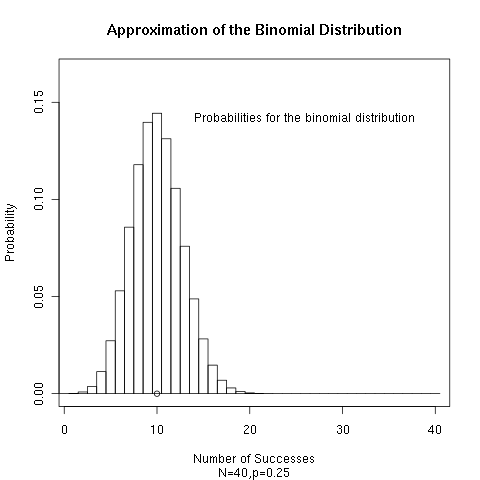
\includegraphics[width=6cm]{img/binomialN40}}
  \only<2>{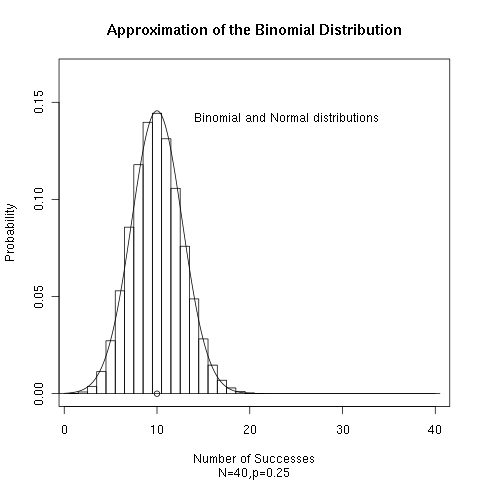
\includegraphics[width=6cm]{img/binomialApproximationN40}}
  
\end{frame}

\section{Examples}

\begin{frame}{Example}
  You want to take a poll of eighty employees. You will ask them if
  they like their benefits package. You suspect that 35\% of all
  employees do like their benefits. What is the probability that
  twenty-two or less will say they do?
\end{frame}


\begin{frame}{Example}
  You want to take a poll of eighty employees. You will ask them if
  they like their benefits package. You suspect that 35\% of all
  employees do like their benefits. Determine the cut-off where there
  is a twenty-five percent chance that fewer than the cut-off will say
  they do like their benefits.
\end{frame}


\begin{frame}{Clicker Quiz}
  Clarkson University claims that over eighty percent of all students
  take part in intramural sports. You choose three hundred students at
  random. What is the probability that more than two-hundred and fifty will say
  that they take part in intramural sports?

  \vfill

  \begin{tabular}{l@{\hspace{3em}}l@{\hspace{3em}}l}
    A: 0.0643  & B: 0.4679 & C: 0.9375
  \end{tabular}

  \vfill
  \vfill
  \vfill

\end{frame}



% LocalWords:  Clarkson pausesection hideallsubsections


%\part{}
\lecture{Sample Distributions}{sample-distributions}


\title{Sample Distributions}
\subtitle{The Sample Mean Varies}

\author{Kelly Black}
\institute{Clarkson University}
\date{24 Feb 2012}

\begin{frame}
  \titlepage
\end{frame}

\begin{frame}
  \frametitle{Outline}
  \tableofcontents[pausesection,hideallsubsections]
\end{frame}


\section{Clicker Quiz}


\begin{frame}{Clicker Quiz}

  Clarkson University claims that over eighty percent of all students
  take part in intramural sports. You choose three hundred students at
  random. What is the probability that more than two-hundred and fifty will say
  that they take part in intramural sports?

  \vfill

  \begin{tabular}{l@{\hspace{3em}}l@{\hspace{3em}}l}
    A: 0.0643  & B: 0.4679 & C: 0.9375
  \end{tabular}

  \vfill
  \vfill
  \vfill

\end{frame}




\section{Coin Flip}

\begin{frame}
  \frametitle{Coin Flip}

  Flip a Coin

  \only<2->{How many tails?}

  \only<3->{Divide by the number of people.}

  \only<4->{Do it again.}

  \only<5->{Do it again.}

\end{frame}

\section{The Sample Mean}

\begin{frame}
  \frametitle{Sample Mean}

  We have a bunch of measurements:
  \begin{eqnarray*}
    \bar{x} & = & x_1,~x_2,~x_3,\cdots,~x_n.
  \end{eqnarray*}
  Each measurement has a mean, $\mu$, and a standard deviation of
  $\sigma$. We assume that they are all independent of one another.
  
  \only<1-2>
  {
    \begin{definition}
      Given measurements the sample mean is 
      \begin{eqnarray*}
        \bar{x} & = & \frac{x_1+x_2+x_3+\cdots+x_n}{n}.
      \end{eqnarray*}
    \end{definition}
  }

  \only<3->
  {
    \begin{definition}
      Given measurements the sample mean is 
      \begin{eqnarray*}
        \bar{x} & = & \frac{x_1+x_2+x_3+\cdots+x_n}{n}.
      \end{eqnarray*}
      The sample mean, $\bar{x}$,  has a mean of $\mu$, and it has a
      standard deviation of $\frac{\sigma}{\sqrt{n}}$.
    \end{definition}
  }


  \only<2->
  {
    The sample mean is a random variable!
  }

\end{frame}


\begin{frame}
  (central limit theorem example)
\end{frame}

\section{Examples}

\begin{frame}
  \frametitle{}

  A random variable has a mean of 3.0 and a standard deviation of
  4.5. If I take one sample what is the probability that it is less
  than zero?

  \vfill

  \only<2->
  {
    If I take four samples what is the probability that it is less
    than zero?
  }

  \vfill

\end{frame}


\begin{frame}
  \frametitle{Clicker Quiz}

  The total change in a stock's price on one particular day has a mean
  of -.35\$ with a standard deviation of .86\$. A sample of 16 stocks
  is taken. What is the probability that the mean will be more than
  zero?

  \vfill

  \begin{tabular}{l@{\hspace{3em}}l@{\hspace{3em}}l@{\hspace{3em}}l}
    A: 0.0516  & B: 0.3420 & C: 0.6580 & D: 0.9484
  \end{tabular}

  \vfill
  \vfill
  \vfill

\end{frame}


\begin{frame}
  \frametitle{Example}

  I have a random variable. It is normally distributed with a mean of
  0.5 and a standard deviation of 2.0. How many samples should I take
  so that
  \begin{eqnarray*}
    p(\bar{x} < 0.25) & = & 0.05?
  \end{eqnarray*}

\end{frame}




% LocalWords:  Clarkson pausesection hideallsubsections



% %%%%%%%%%%%%%%%%%%%%%%%%%%%%%%%%%%%%%%%%%%%%%%%%%%%%%%%%%%%%


\lecture{More Sample Distributions}{more-sample-distributions}
\section{More Sample Distributions}

\title{More Sample Distributions}
\subtitle{More Examples}

\author{Kelly Black}
\institute{Clarkson University}
\date{Feb 27, 2012}

\begin{frame}
  \titlepage
\end{frame}

\begin{frame}
  \frametitle{Outline}
  \tableofcontents[pausesection,hideothersubsections,sectionstyle=show/hide]
\end{frame}


\subsection{Clicker Quiz}


\begin{frame}
  \frametitle{Clicker Quiz}

  The mass of the contents of a product are normally distributed with
  a mean of 0.35 kg and a standard deviation of 0.04 kg. What is the
  probability that the sample mean of four samples will be less than
  0.33 kg?

  \vfill

  \begin{tabular}{l@{\hspace{3em}}l@{\hspace{3em}}l@{\hspace{3em}}l}
    A: 0.0228  & B: 0.1318  & C: 0.1587
  \end{tabular}

  \vfill
  \vfill
  \vfill

\end{frame}

\subsection{The Sample Mean}

\begin{frame}
  \frametitle{Sample Mean}

  We have a bunch of measurements:
  \begin{eqnarray*}
    \bar{x} & = & x_1,~x_2,~x_3,\cdots,~x_n.
  \end{eqnarray*}
  Each measurement has a mean, $\mu$, and a standard deviation of
  $\sigma$. We assume that they are all independent of one another.
  
    \begin{definition}
      Given measurements the sample mean is 
      \begin{eqnarray*}
        \bar{x} & = & \frac{x_1+x_2+x_3+\cdots+x_n}{n}.
      \end{eqnarray*}
      The sample mean, $\bar{x}$,  has a mean of $\mu$, and it has a
      standard deviation of $\frac{\sigma}{\sqrt{n}}$.
    \end{definition}

    The sample mean is a random variable!

\end{frame}


\subsection{Examples}

\begin{frame}
  \frametitle{Example}

  The life time of batteries is normally distributed with a mean of
  19.8 hours and a standard deviation of 1.3 hours. What is the
  probability that a sample size of six batteries will give a sample
  mean that is more than 21.1 hours?

\end{frame}


\begin{frame}
  \frametitle{Example}

  You want to estimate the start up costs for restaurants in an
  area. If the mean start up costs are \$235,000 with a standard
  deviation of \$45,000 what is the probability that a sample of
  twenty restaurants will be between \$260,000 and \$205,000?

\end{frame}


\begin{frame}
  \frametitle{Example}

  You want to estimate the start up costs for restaurants in an
  area. If the mean start up costs are \$235,000 with a standard
  deviation of \$45,000 how many restaurants should you poll so that
  the probability to be within \$1,000 of the mean is ten percent?

\end{frame}


\begin{frame}
  \frametitle{Clicker Quiz}

  You want to estimate the start up costs for restaurants in an
  area. The mean start up costs are \$235,000 with a standard
  deviation of \$45,000. What is the probability that twenty samples
  will give a sample mean greater than \$245,000?


  \vfill

  \begin{tabular}{l@{\hspace{3em}}l@{\hspace{3em}}l@{\hspace{3em}}l}
    A: 0.1611  & B: 0.4121  & C: 0.9999
  \end{tabular}

  \vfill
  \vfill
  \vfill

\end{frame}



% LocalWords:  Clarkson pausesection hideallsubsections


%\part{}
\lecture{Confidence Intervals}{confidence-interval}


\title{The Confidence Interval}
\subtitle{Introducing the Idea}

\author{Kelly Black}
\institute{Clarkson University}
\date{29 February 2012}

\begin{frame}
  \titlepage
\end{frame}

\begin{frame}
  \frametitle{Outline}
  \tableofcontents[pausesection,hideallsubsections]
\end{frame}


\section{Clicker Quiz}


\begin{frame}
  \frametitle{Clicker Quiz}

  You sample a random variable which has a mean of 2.1 and a standard
  deviation of 4.5. You take 30 samples. What is the probability that
  the sample mean is more than 3.5?

  \vfill

  \begin{tabular}{l@{\hspace{3em}}l@{\hspace{3em}}l@{\hspace{3em}}l}
    A: 0.0446  & B: 0.6221  & C: 0.9954
  \end{tabular}

  \vfill
  \vfill
  \vfill

\end{frame}

\section{The Confidence Interval}


\begin{frame}
  \frametitle{Problem!}

  We have a random variable. It has a mean, $\mu$, and a standard
  deviation, $\sigma$. How do we know?

  \vfill

  \only<2->
  {
    \begin{block}{Example}
      We run a capitol investment firm. Someone asks us for \$250,000
      to start a restaurant. It this a reasonable amount?
    \end{block}
  }

  \vfill

\end{frame}


\begin{frame}{The Big Question}

  How do we estimate the mean of a random variable?
  
\end{frame}


\begin{frame}{Example}
  
  We call up ten restaurant owners and ask them for the amount they
  needed to get started. We then calculate a \textit{sample mean},
  \begin{eqnarray*}
    \bar{x} & = & \frac{x_1 + x_2 + x_3 + x_4 + x_5 + x_6 + x_7 + x_8 + x_9 + x_{10}}{10}.
  \end{eqnarray*}
  This is our \textbf{estimate} for the mean.
  
\end{frame}


\begin{frame}
  \frametitle{Clicker Quiz}

  We call up ten restaurant owners and ask them for the amount they
  needed to get started. We then calculate a \textit{sample mean},
  \begin{eqnarray*}
    \bar{x} & = & \frac{x_1 + x_2 + x_3 + x_4 + x_5 + x_6 + x_7 + x_8 + x_9 + x_{10}}{10}.
  \end{eqnarray*}

  Is this estimate close to the true mean?

  \vfill

  \begin{tabular}{l@{\hspace{3em}}l@{\hspace{3em}}l@{\hspace{3em}}l}
    A: Yes  & B: No  & C: Maybe??
  \end{tabular}

  \vfill
  \vfill
  \vfill

  *
\end{frame}


\begin{frame}{Estimators}

  \begin{definition}{Bias}
    \begin{itemize}
    \item If our estimator for a parameter is expected to be less that
      the true value is has a \textit{negative bias.}
    \item If our estimator for a parameter is expected to be more that
      the true value is has a \textit{positive bias.}
    \item If the expectation of our estimator for a parameter is the
      same as the true value then it is \textit{unbiased.}
    \end{itemize}
  \end{definition}
  
  \vfill

\end{frame}


\begin{frame}{Estimator - An example}

  \begin{definition}{Estimator of the mean}
    The sample mean is an estimator of the mean,
  \begin{eqnarray*}
    \bar{x} & = & \frac{x_1 + x_2 + x_3 + \cdots + x_{n}}{n}.
  \end{eqnarray*}    
  \end{definition}
  
  \vfill
  \vfill
  \vfill

  *
\end{frame}



\begin{frame}
  \frametitle{Estimator for the mean}


  \only<1>{\centerline{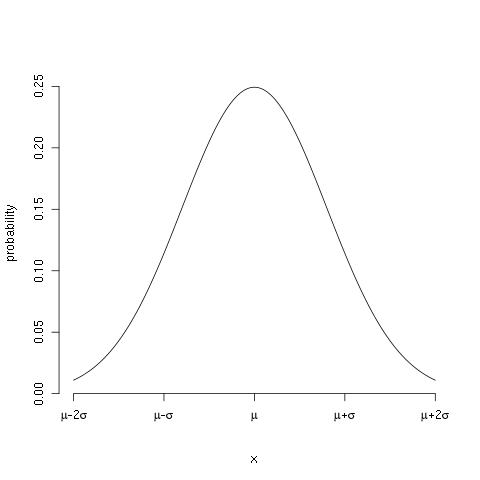
\includegraphics[width=6cm]{img/week8Dist}}}
  \only<2>{\centerline{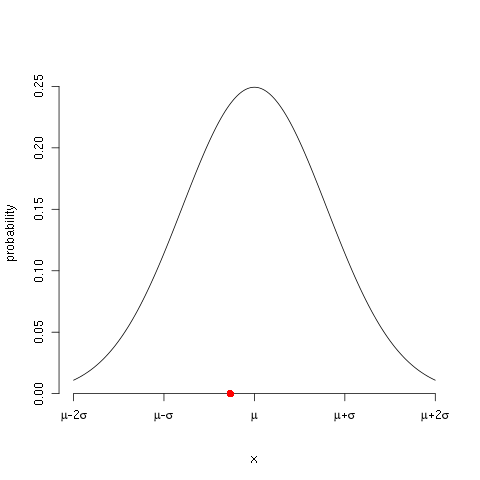
\includegraphics[width=6cm]{img/week8DistSample}}}
  \only<3>{\centerline{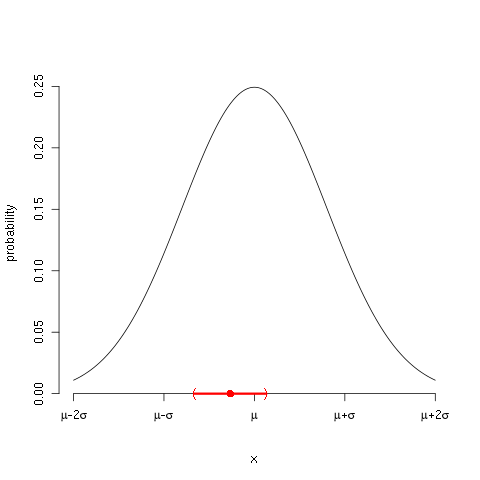
\includegraphics[width=6cm]{img/week8DistConfInterval}}}

\end{frame}



\begin{frame}
  \frametitle{Clicker Quiz}


  \centerline{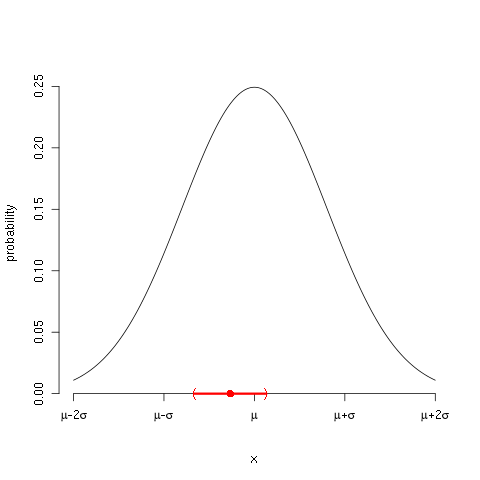
\includegraphics[width=6cm]{img/week8DistConfInterval}}
  If the value of $\alpha$ is increased does the length of the
  ``error'' increase or decrease?  \vfill

  \begin{tabular}{l@{\hspace{3em}}l@{\hspace{3em}}l@{\hspace{3em}}l}
    A: Increase  & B: Decrease
  \end{tabular}

  \vfill
  \vfill
  \vfill

\end{frame}



\begin{frame}
  \frametitle{Example}

  We contact ten restaurant owners and ask what their starting costs
  were. We get a sample mean of \$235,000 and a standard deviation of
  \$45,000. Find the 95\% confidence interval.

\end{frame}


% LocalWords:  Clarkson pausesection hideallsubsections



\lecture{Confidence Intervals Part II}{confidence-interval-II}
\section{Confidence Intervals Part II}

\title{Confidence Intervals}
\subtitle{Part II - Putting them to Use}

%\author{Kelly Black}
%\institute{Clarkson University}
\date{2 March 2012}

\begin{frame}
  \titlepage
\end{frame}

\begin{frame}
  \frametitle{Outline}
  \tableofcontents[pausesection,hideothersubsections,sectionstyle=show/hide]
\end{frame}


\subsection{Clicker Quiz}


\begin{frame}
  \frametitle{Clicker Quiz}

  You run an experiment multiple times. Each time you generate data
  and calculate a sample mean. The sample means are plotted below with
  circles, and the true mean is the square. The estimator appears to
  be \rule{3cm}{.2mm} .

  \vfill

  \centerline{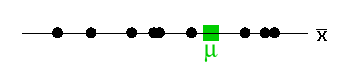
\includegraphics[width=5cm]{img/negativeBias}}

  \vfill

  \begin{tabular}{l@{\hspace{3em}}l@{\hspace{3em}}l@{\hspace{3em}}l}
    A: Negatively Biased  & B: Unbiased  & C: Positively Biased
  \end{tabular}

  \vfill
  \vfill
  \vfill

\end{frame}


\subsection{Confidence Intervals}


\begin{frame}

  \centerline{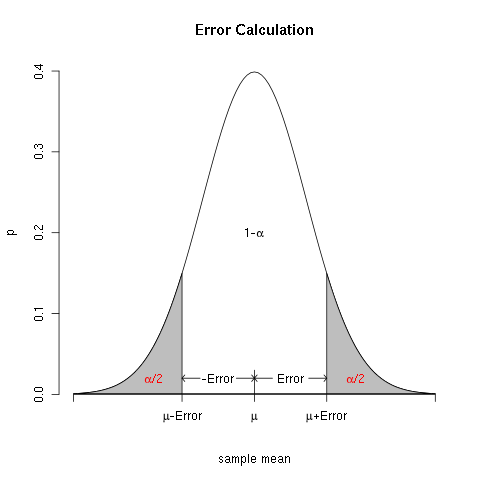
\includegraphics[width=6cm]{img/confidenceInterval}}

  \begin{block}{The Error Relationship for Confidence Intervals}
    \begin{eqnarray*}
      p\lp z \leq \frac{-error}{\frac{\sigma}{\sqrt{n}}}\rp & = & \frac{\alpha}{2}.
    \end{eqnarray*}
  \end{block}

\end{frame}


\begin{frame}{The Confidence Interval}
  \begin{definition}
    The \textit{confidence interval} is an interval that likely
    includes the true mean.
  \end{definition}
\end{frame}

\subsection{Examples}


\begin{frame}
  \frametitle{Example}

  We call up and ask twenty factory operators in a given sector what
  their yearly output is in dollars. The sample mean is \$450,000 and
  the standard deviation is \$50,000. Find the 95\% confidence
  interval.

  \vfill

  \only<2->{
    \textit{
      The 95\% confidence interval is from \$471,913 and \$428,087
      assuming a normal distribution with twenty samples.
    }
  }

  \vfill

\end{frame}


\begin{frame}
  \frametitle{Example}

  You read a report that says that eighteen companies in a given
  sector were polled, and the confidence interval for the yearly
  output in dollars is between \$710,000 and \$650,000 with a standard
  deviation of \$96,000. What is the significance level?

  \vfill

  \only<2->{
    \textit{
      There is a probability of about 18\% that the true mean is not
      between \$710,000 and \$650,000.
    }
  }

  \vfill

\end{frame}


\begin{frame}
  \frametitle{Example}

  You are asked to determine a 95\% confidence interval for the mean
  yearly output in dollars for the companies in a given sector. You
  are told that the error should be about \$30,000. From the reports
  that you have read it looks like the standard deviation is about
  \$100,000. How many companies should you poll?

  \vfill

  \only<2->{
    \textit{
      Assuming a normal distribution you will need to poll at least 43
      companies to get a 95\% confidence interval with an error of \$30,000.
    }
  }

  \vfill


\end{frame}



% LocalWords:  Clarkson pausesection hideallsubsections



% %%%%%%%%%%%%%%%%%%%%%%%%%%%%%%%%%%%%%%%%%%%%%%%%%%%%%%%%%%%%

%\part{}
\lecture{Introduction to Hypothesis Testing}{intro-to-hypothesis-testing}


\title{Introduction to Hypothesis Testing}
\subtitle{Is there a difference? (yes/no)}

\author{Kelly Black}
\institute{Clarkson University}
\date{9 March 2012}

\begin{frame}
  \titlepage
\end{frame}

\begin{frame}
  \frametitle{Outline}
  \tableofcontents[pausesection,hideallsubsections]
\end{frame}


\section{Clicker Quiz}


\begin{frame}
  \frametitle{Clicker Quiz}

  A random variable has a mean of 3.7 and a standard deviation of
  1.2. What is the probability that a sample mean using six samples is
  more than 4.1?

  \vfill

  \begin{tabular}{l@{\hspace{3em}}l@{\hspace{3em}}l@{\hspace{3em}}l}
    A: 0.2061  & B: 0.7939  & C: 0.8165
  \end{tabular}

  \vfill
  \vfill
  \vfill


\end{frame}




\section{Introduction To Hypothesis Testing}

\begin{frame}
  \frametitle{Introduction To Hypothesis Testing}

  I \textbf{\underline{think}} that a random variable has a mean of 3.7
  and a standard deviation of 1.2. I take six samples and get a sample
  mean of 4.1. Is the mean really 3.7?

  \vfill

  \only<2->{Maybe!}

  \vfill

\end{frame}


\begin{frame}
  \frametitle{The Problem}

  Situation: We think that $\mu$ is  some number.

  Problem: $\bar{x}$ is a random variable.

  Problem\textsuperscript{2}: $\bar{x}$ is our only way of estimating $\mu$!

\end{frame}

\begin{frame}{What do we do?}

  \begin{enumerate}
  \item<1-> We have some idea/belief of what to expect.
  \item<2-> This is our hypothesis of what we \textit{think} is happening.
  \item<3-> We want to make a case for some change in how we interpret the
    situation.
  \item<4-> Assume that the status quo is good or better. (Call this the
    \textit{Null Hypothesis}, $H_0$.)
  \item<5-> Construct a hypothesis about what we think is \textbf{think}
    is happening. (Call this the \textit{alternate hypothesis}, $H_a$.)
  \item<6-> Collect evidence assuming $H_0$ is true. 
  \item<7-> If the evidence is \textit{``highly unlikely''} under the
    assumed conditions then reject the null hypothesis, otherwise we
    cannot reject the null hypothesis.
  \end{enumerate}
  
\end{frame}

\section{Examples}

\begin{frame}{Example}

  We think that interest rates for mortgages have decreased since last
  quarter.

  \vfill

  \only<2->
  {
    \begin{tabular}{l@{\hspace{2em}}l}
      $H_0$: & Interest rates are the same. \\
      $H_a$: & Interest rates have decreased.
    \end{tabular}
  }

  \vfill

  \only<3->
  {
    Sample fifteen banks, find the mean interest rate, and ask if
    there is sufficient evidence to reject $H_0$.
  }

  \vfill

\end{frame}

\begin{frame}{Example}

  We think that foreclosures have increased since last quarter.

  \vfill

  \only<2->
  {
    \begin{tabular}{l@{\hspace{2em}}l}
      $H_0$: & Foreclosure rates are the same. \\
      $H_a$: & Foreclosure rates have increased.
    \end{tabular}
  }

  \vfill

  \only<3->
  {
    Sample thirty properties at random, calculate a foreclosure rate, and ask if
    there is sufficient evidence to reject $H_0$.
  }

  \vfill

\end{frame}


\begin{frame}{Example}

  We think that a new commercial will change the demand for a product.

  \vfill

  \only<2->
  {
    \begin{tabular}{l@{\hspace{2em}}l}
      $H_0$: & The commercial has no impact. \\
      $H_a$: & The commercial has an impact.
    \end{tabular}
  }

  \vfill

  \only<3->
  {
    Play the commercial in ten markets. Monitor the sales in those markets, and ask if
    there is sufficient evidence to reject $H_0$.
  }

  \vfill

\end{frame}


\begin{frame}{Three Options!}

  In the proceeding examples there were three different options:
  \begin{itemize}
  \item Decrease,
  \item Increase,
  \item Change.
  \end{itemize}
  
\end{frame}


\begin{frame}{Example}

  We think that interest rates for mortgages have
  \textcolor{red}{\textbf{decreased}} since last quarter.

  \vfill

    \begin{tabular}{l@{\hspace{2em}}l}
      $H_0$: & Interest rates are the same. \\
      $H_a$: & Interest rates have \textcolor{red}{\textbf{decreased}}.
    \end{tabular}

  \vfill

    Sample fifteen banks, find the mean interest rate, and ask if
    there is sufficient evidence to reject $H_0$.

  \vfill

\end{frame}

\begin{frame}{Example}

  We think that foreclosures have \textcolor{red}{\textbf{increased}} since last quarter.

  \vfill

    \begin{tabular}{l@{\hspace{2em}}l}
      $H_0$: & Foreclosure rates are the same. \\
      $H_a$: & Foreclosure rates have \textcolor{red}{\textbf{increased}}.
    \end{tabular}

  \vfill

    Sample theory properties at random, calculate a foreclosure rate, and ask if
    there is sufficient evidence to reject $H_0$.

  \vfill

\end{frame}


\begin{frame}{Example}

  We think that a new commercial will \textcolor{red}{\textbf{change}} the demand for a product.

  \vfill

    \begin{tabular}{l@{\hspace{2em}}l}
      $H_0$: & The commercial has no impact. \\
      $H_a$: & The commercial has \textcolor{red}{\textbf{an impact}}.
    \end{tabular}

  \vfill

    Play the commercial in ten markets. Monitor the sales in those markets, and ask if
    there is sufficient evidence to reject $H_0$.

  \vfill

\end{frame}


\begin{frame}{Problem}

  \vfill

  $\bar{x}$ is a random variable.

  \vfill

  The data can \textbf{lie}!

  \vfill
  
\end{frame}


\begin{frame}{The Possibilities}

  \begin{eqnarray*}
    \mathrm{Data~-} & &
      \begin{array}{l@{\hspace{1em}}|l|l|} 
        \multicolumn{1}{c}{~} & \multicolumn{1}{c}{H_0 \mathrm{~is~true}} & \multicolumn{1}{c}{H_0 \mathrm{~is~false}} \\ 
               \hhline{~--}
        \mathrm{Do~Not~Reject~}H_0 & \mathrm{good!} & \mathrm{Type~II~Error} \\ \hhline{~|-|-|}
        \mathrm{Reject~}H_0 & \mathrm{Type~I~Error} & \mathrm{good!} \\ \hhline{~--}
      \end{array}
  \end{eqnarray*}
  
\end{frame}


\begin{frame}{How To State Results}

  How you state your conclusions matter! It is an ethical issue in
  terms of conveying your assumptions and potential problems
  associated with the methodology.

  \begin{block}{Reject $H_0$}
    There is sufficient evidence to reject $H_0$ at the \#
    significance level assuming a normal distribution and a \#
    standard deviation.
  \end{block}

  \begin{block}{Cannot Reject $H_0$}
    There is not sufficient evidence to reject $H_0$ at the \#
    significance level assuming a normal distribution and a \#
    standard deviation.
  \end{block}

  
\end{frame}

\begin{frame}{The Methodology}

  What do we do?

  \begin{enumerate}
  \item Assume that $H_0$ is true.
  \item Ask, ``Are the data an unlikely result?''
  \end{enumerate}

  \only<2->
  {
    We want:
    \begin{itemize}
    \item The probability that we get our result to be ``small.''
    \item The probability that we get our result \textit{given our
        assumptions} is the significance level ($\alpha$). \textbf{It is
        a conditional probability!}
    \end{itemize}
  }

  \only<3->
  {
    Note: We need to define this cut-off value, $\alpha$, \textbf{in
      advance!} i.e. before any data collection or manipulation.
  }
  
\end{frame}


\begin{frame}{Example}

  I see a publication that says that the mean house value in an area
  is \$215,000 with a standard deviation of \$35,000. I think that
  this is too high.

  \vfill

  \only<2->
  {

    \begin{tabular}{l@{\hspace{2em}}l}
      $H_0$: & The mean house price is \$215,000 or more. \\
      $H_a$: & The mean house price is \textcolor{red}{\textbf{more than \$215,000}}.
    \end{tabular}

    I will use a 5\% significance level.

  }

  \vfill

  \only<3->
  {

    Suppose that I take a random sample of ten homes and get a sample
    mean of \$198,000. Is the mean house price smaller than \$215,000?

  }

  \vfill

  
  
\end{frame}

% LocalWords:  Clarkson pausesection hideallsubsections


%\part{}
\lecture{Hypothesis Testing}{hypothesis-testing}


\title{Hypothesis Testing}
\subtitle{Is there a difference?}

\author{Kelly Black}
\institute{Clarkson University}
\date{12 March 2012}

\begin{frame}
  \titlepage
\end{frame}

\begin{frame}
  \frametitle{Outline}
  \tableofcontents[pausesection,hideallsubsubsections]
\end{frame}


\section{Clicker Quiz}


\begin{frame}
  \frametitle{Clicker Quiz}

  Cereal is produced at one of your factories. You are told that the
  mean contents is 417.3g per box. You suspect that this is too
  high. 

  What hypothesis test would you form to test this? \\
  ~ \\
  \begin{tabular}{ll@{\hspace{3em}}l}
    A & $H_0$: The mean is less that 417.3g  \\
      & $H_a$: The mean is  417.3g \\
    ~ \\
    B & $H_0$: The mean is 417.3g \\
      & $H_a$: The mean is more than 417.3g \\
      ~ \\
      C & $H_0$: The mean is 417.3kg  \\
        & $H_a$: The mean is less than 417.3kg 
  \end{tabular}

\end{frame}


\section{Examples}

\subsection{Cereal Box Contents}

\begin{frame}{Cereal}

  Cereal is produced at one of your factories. You are told that the
  mean contents is 417.3g per box. You suspect that this is too
  high. 

  \vfill

  \only<2->
  {
    \begin{tabular}{l@{\hspace{2em}}l}
      $H_0$: & The mean is 417.3g \\
      $H_a$: & The mean is less than 417.3g 
    \end{tabular}
    \\ Use a 5\% significance level.
  }

  \vfill

  \only<3->
  {

    Sample fifteen boxes chosen at random, and ask if there is
    sufficient evidence to reject $H_0$. Suppose we find a sample mean
    of 412.4g and a standard deviation of 12.0g.

  }

  \vfill

\end{frame}

\begin{frame}{Result}

  We \textbf{do not} have sufficient evidence to reject $H_0$ at the
  5\% significance level using a normal distribution with fifteen
  samples and a standard deviation of 12.0g.
  
\end{frame}



\subsection{Stock Price Change}
\begin{frame}
  \frametitle{Clicker Quiz}

  We read that the mean change in the price of the stocks in a given
  sector changed by -0.55\$ with a standard deviation of 0.74\$. We
  suspect that the mean change is not that low.

  What hypothesis test would you form to test this? \\
  ~ \\
  \begin{tabular}{ll@{\hspace{3em}}l}
    A & $H_0$: The mean change is -0.55\$. \\
      & $H_a$: The mean change is more than -0.55. \\
    ~ \\
    B & $H_0$: The mean change is -0.55\$. \\
      & $H_a$: The mean change is less than -0.55\$. \\
    ~ \\
    C & $H_0$: The mean change is less than -0.55\$.  \\
      & $H_a$: The mean change is -0.55\$. \\
    ~ \\
    D & $H_0$: The mean change is more than -0.55\$.  \\
      & $H_a$: The mean change is -0.55\$.

  \end{tabular}

\end{frame}


\begin{frame}{Stock Price}

  We read that the mean change in the price of the stocks in a given
  sector changed by -0.55\$ with a standard deviation of 0.74\$. We
  suspect that the mean change is not that low.

  \vfill

  \only<2->
  {
    \begin{tabular}{l@{\hspace{2em}}l}
      $H_0$: & The mean change is -0.55\$. \\
      $H_a$: & The mean change is more than -0.55. 
    \end{tabular}
    \\ Use a 5\% significance level.
  }

  \vfill

  \only<3->
  {

    Sample one-hundred stocks chosen at random, and ask if there is
    sufficient evidence to reject $H_0$. Suppose that we find a sample
    mean of -0.42\$.

  }

  \vfill

\end{frame}

\begin{frame}{Result}

  We have sufficient evidence to reject $H_0$ at the 5\% significance
  level using a normal distribution with a one-hundred samples and a
  standard deviation of 0.74\$.
  
\end{frame}


\subsection{Units Shipped}
\begin{frame}
  \frametitle{Clicker Quiz}

  You are told that the mean number of units shipped per day at a
  particular factory is 135,000 units per day. You think that number
  is not correct.

  What hypothesis test would you form to test this? \\
  ~ \\
  \begin{tabular}{ll@{\hspace{3em}}l}
    A & $H_0$: The mean number of units is more than 135,000 units per day. \\
      & $H_a$: The mean number of units is 135,000 units per day. \\
    ~ \\
    B & $H_0$: The mean number of units is 135,000 units per day. \\
      & $H_a$: The mean number of units is more than 135,000 units per day. \\
    ~ \\
    C & $H_0$: The mean number of units is 135,000 units per day.  \\
      & $H_a$: The mean number of units is not 135,000 units per day. \\
    ~ \\
    D & $H_0$: The mean number of units is not 135,000 units per day.  \\
      & $H_a$: The mean number of units is 135,000 units per day.

  \end{tabular}

\end{frame}


\begin{frame}{Units Shipped}


  You are told that the mean number of units shipped per day at a
  particular factory is 135,000 units per day. You think that number
  is not correct.

  \vfill

  \only<2->
  {
    \begin{tabular}{l@{\hspace{2em}}l}
      $H_0$: & The mean number of units is 135,000 units per day. \\
      $H_a$: & The mean number of units is not 135,000 units per day.
    \end{tabular}
    \\ Use a 5\% significance level.
  }

  \vfill

  \only<3->
  {

    Sample the daily output for twenty-five days chosen at random, and
    ask if there is sufficient evidence to reject $H_0$. Suppose we
    find a sample mean of 140,266 units per day and a standard
    deviation of 14,000 units per day.

  }

  \vfill

\end{frame}

\begin{frame}{Result}

  We \textbf{do not} have sufficient evidence to reject $H_0$ at the
  5\% significance level using a normal distribution with twenty-five
  samples and a standard deviation of 14,000 units per day.
  
\end{frame}



% LocalWords:  Clarkson pausesection hideallsubsections




% %%%%%%%%%%%%%%%%%%%%%%%%%%%%%%%%%%%%%%%%%%%%%%%%%%%%%%%%%%%%



\lecture{Hypothesis Testing with the Classical Approach}{hypothesis-testing-classical}
\section{Hypothesis Testing with the Classical Approach}

\title{Hypothesis Testing Again}
\subtitle{The ``Classical'' Approach}

%\author{Kelly Black}
%\institute{Clarkson University}
\date{14 March 2012}

\begin{frame}
  \titlepage
\end{frame}

\begin{frame}
  \frametitle{Outline}
  \tableofcontents[pausesection,hideothersubsections,sectionstyle=show/hide]
\end{frame}


\subsection{Clicker Quiz}


\begin{frame}
  \frametitle{Clicker Quiz}

  \iftoggle{clicker}{%

    I read in the \textit{Integrator} that the mean height of Clarkson
    students is 180.0 cm with a standard deviation of 14.0 cm. I think
    that this is too high and sample twenty students chosen at random
    to find a sample mean of 175.1 cm. Are my suspicions correct? (Use
    a 5\% significance level.)

    \vfill

    \begin{tabular}{l@{\hspace{3em}}l}
      A: & There is sufficient evidence to reject $H_0$.  \\
      B: & There is not sufficient evidence to reject $H_0$.  
    \end{tabular}

    \vfill
    \vfill
    \vfill

    

  }


\end{frame}

\subsection{Classical Approach}

\begin{frame}
  \frametitle{What if....}


  I read in the \textit{Integrator} that the mean height of Clarkson
  students is 180.0 cm with a standard deviation of 14 cm. I think
  that this is too high and sample twenty students chosen at random to
  find a sample mean of \textbf{174.7} cm. Are my suspicions correct?
  (Use a 5\% significance level.)

    \vfill
    

\end{frame}


\begin{frame}{Result}

  We have sufficient evidence to reject $H_0$ at the 5\% significance
  level using a normal distribution with twenty samples and a standard
  deviation of 14.0cm.
  
\end{frame}





\begin{frame}{Clicker Quiz}

  \iftoggle{clicker}{%

    I see a publication that says that the mean house value in an area
    is \$215,000 with a standard deviation of \$35,000. I think that
    this is too low.  Suppose that I take a random sample of fifteen
    homes and get a sample mean of \$232,000.

    \vfill 

    What is the $z$-statistic?

    \begin{tabular}{l@{\hspace{3em}}l@{\hspace{3em}}l@{\hspace{3em}}l}
      A: -1.881  & B: -1.644  & C: 1.644 & D: 1.881
    \end{tabular}

    \vfill
    \vfill
    \vfill

  }

\end{frame}

\begin{frame}{Result}

  We have sufficient evidence to reject $H_0$ at the 5\% significance
  level using a normal distribution with fifteen samples and a standard
  deviation of \$35,000.
  
\end{frame}


\begin{frame}{Clicker Quiz}

  \iftoggle{clicker}{%

    \begin{eqnarray*}
      \begin{array}{lrcl}
        H_0: & \mu & = & 800 \\
        H_a: & \mu & \neq & 800
      \end{array}
    \end{eqnarray*}

    \begin{eqnarray*}
      n & = & 30, \\
      \bar{x} & = & 758,\\
      \sigma & = & 118, \\
      \alpha & = & 0.05.
    \end{eqnarray*}

    \vfill 

    What is the $z$-statistic?

    \begin{tabular}{l@{\hspace{3em}}l@{\hspace{3em}}l@{\hspace{3em}}l}
      A: -1.960  & B: -1.950  & C: -0.065 & D: 1.960
    \end{tabular}

    \vfill
    \vfill
    \vfill

  }

\end{frame}

\begin{frame}{Result}

  We \textbf{do not} have sufficient evidence to reject $H_0$ at the
  5\% significance level using a normal distribution with thirty
  samples and a standard deviation of 118.
  
\end{frame}




% LocalWords:  Clarkson pausesection hideallsubsections



% %%%%%%%%%%%%%%%%%%%%%%%%%%%%%%%%%%%%%%%%%%%%%%%%%%%%%%%%%%%%



\lecture{Hypothesis Testing With The Sample Standard Deviation}{hypothesis-testing-single-sample}
\part{Hypothesis Testing With The Sample Standard Deviation}

\title{Hypothesis Testing}
\subtitle{What if you do not know the true standard deviation?}

\author{Kelly Black}
\institute{Clarkson University}
\date{16 March 2012}

\begin{frame}
  \titlepage
\end{frame}

\begin{frame}
  \frametitle{Outline}
  \tableofcontents[pausesection,hideallsubsections,part=1]
\end{frame}


\section{Clicker Quiz}


\begin{frame}{Clicker Quiz}

  \iftoggle{clicker}{%

    \begin{eqnarray*}
      \begin{array}{lrcl}
        H_0: & \mu & = & 45.0 \\
        H_a: & \mu & \neq & 45.0
      \end{array}
    \end{eqnarray*}

    \begin{eqnarray*}
      n & = & 10, \\
      \bar{x} & = & 49.9,\\
      \sigma & = & 8.0, \\
      \alpha & = & 0.05.
    \end{eqnarray*}

    \vfill 

    What is the \textit{critical} $z$-statistic?

    \begin{tabular}{l@{\hspace{3em}}l@{\hspace{3em}}l@{\hspace{3em}}l}
      A: 0.613  & B: 1.64 & C: 1.94  & D: 1.96 
    \end{tabular}

    \vfill
    \vfill
    \vfill

  }

\end{frame}






\section{Hypothesis Testing}

\begin{frame}
  \frametitle{Left Sided Test}

  \begin{columns}
    \column{0.25\textwidth}
    \begin{eqnarray*}
      \begin{array}{lrcl}
        H_0: & \mu & = & \# \\
        H_a: & \mu & < & \#
      \end{array}
    \end{eqnarray*}

    \column{0.75\textwidth}

    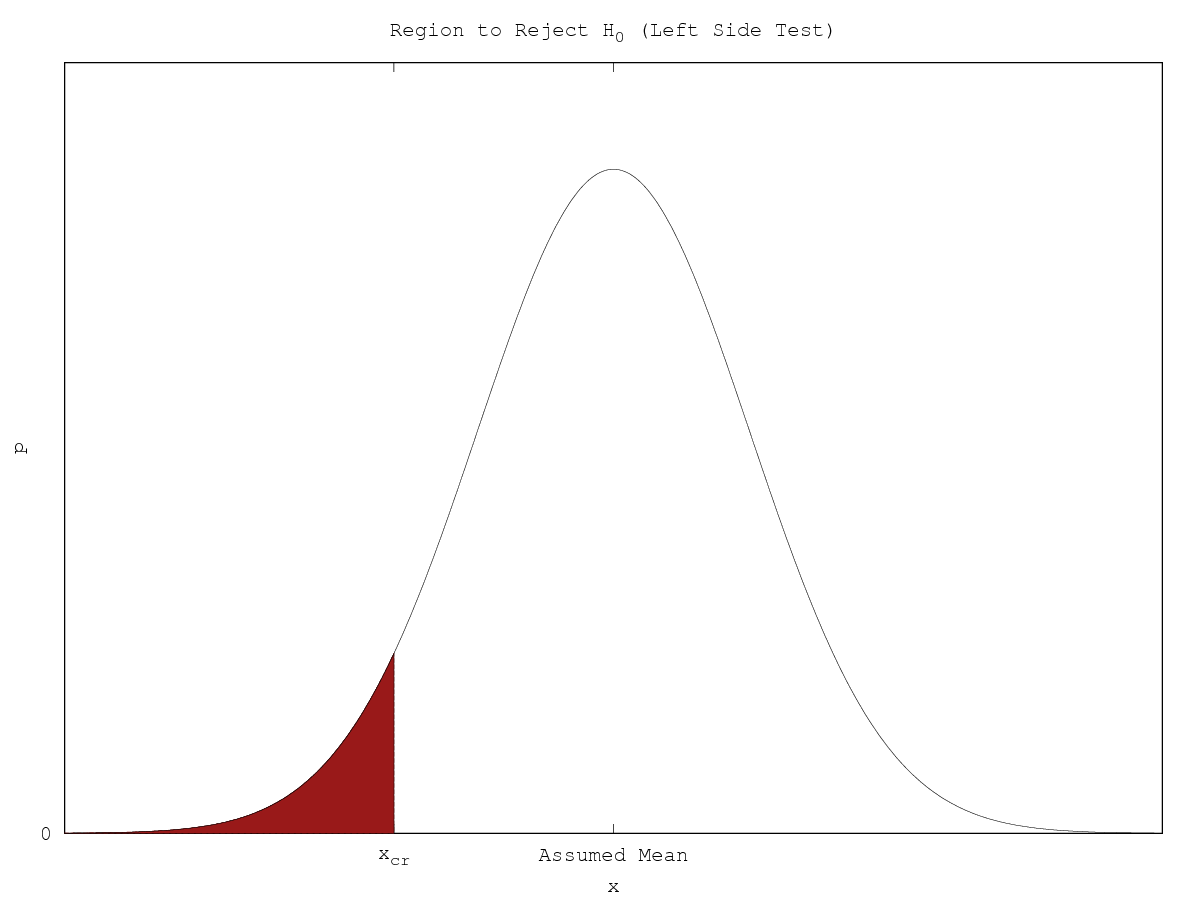
\includegraphics[width=7cm]{img/leftSideHypothesisTest}

  \end{columns}

\end{frame}

\begin{frame}
  \frametitle{Right Sided Test}

  \begin{columns}
    \column{0.25\textwidth}
    \begin{eqnarray*}
      \begin{array}{lrcl}
        H_0: & \mu & = & \# \\
        H_a: & \mu & > & \#
      \end{array}
    \end{eqnarray*}

    \column{0.75\textwidth}

    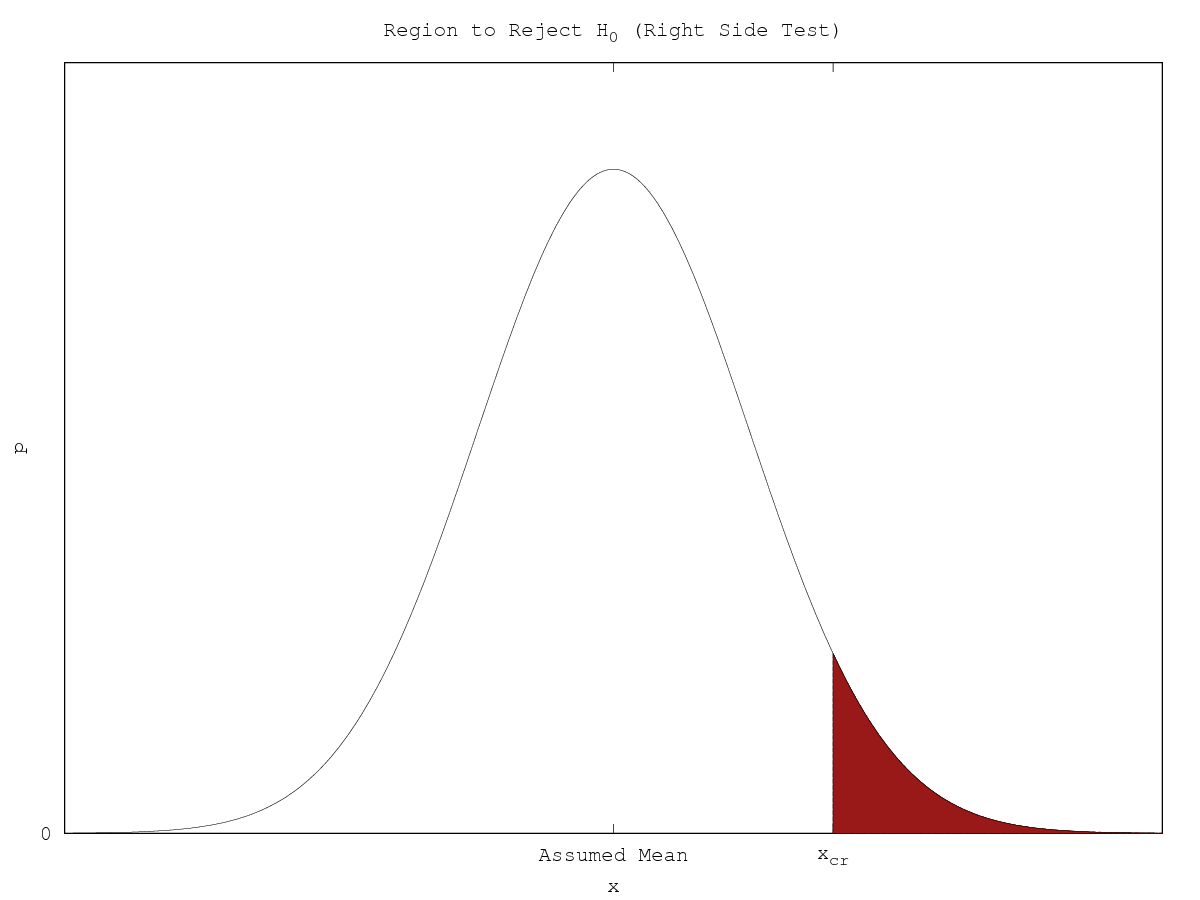
\includegraphics[width=7cm]{img/rightSideHypothesisTest}

  \end{columns}

\end{frame}


\begin{frame}
  \frametitle{Two Sided Test}

  \begin{columns}
    \column{0.25\textwidth}
    \begin{eqnarray*}
      \begin{array}{lrcl}
        H_0: & \mu & = & \# \\
        H_a: & \mu & \neq & \#
      \end{array}
    \end{eqnarray*}

    \column{0.75\textwidth}

    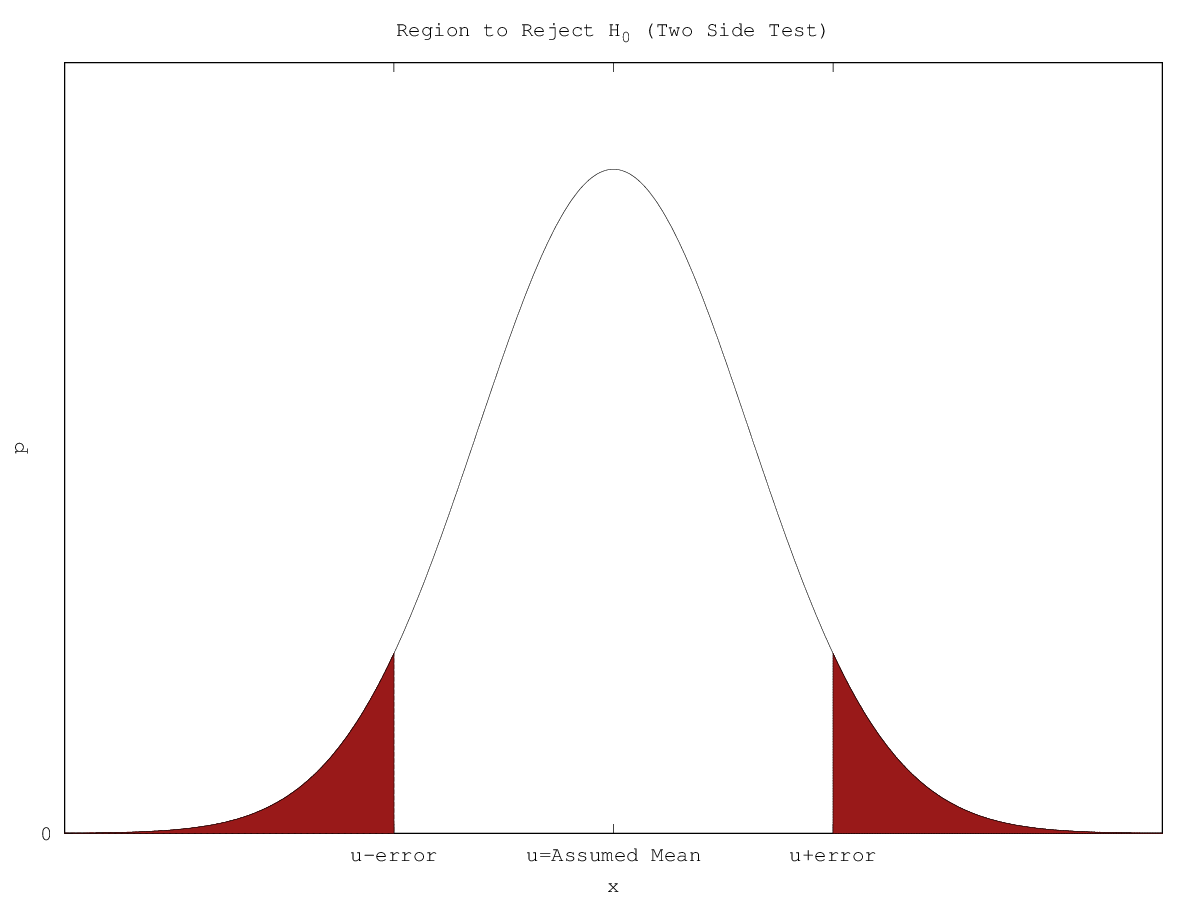
\includegraphics[width=7cm]{img/twoSideHypothesisTest}

  \end{columns}

\end{frame}


\begin{frame}
  \frametitle{Clicker Quiz}

  A supermarket estimates that the mean time spent by customers in a
  store for each visit is about 23.4 minutes with a standard deviation
  of 11.3 minutes. They rearrange one aisle and find a sample mean of
  27.8 minutes. Did the mean time per visit increase? (Use a 5\%
  significance level.)

  \vfill

    \begin{tabular}{l@{\hspace{3em}}l@{\hspace{3em}}l@{\hspace{3em}}l}
      A: Reject $H_0$  & B: Cannot reject $H_0$
    \end{tabular}

    \vfill
    \vfill
    \vfill

\end{frame}


\begin{frame}{The Possibilities}

  \begin{eqnarray*}
    \mathrm{Data~-} & &
      \begin{array}{l@{\hspace{1em}}|l|l|} 
        \multicolumn{1}{c}{~} & \multicolumn{1}{c}{H_0 \mathrm{~is~true}} & \multicolumn{1}{c}{H_0 \mathrm{~is~false}} \\ 
               \hhline{~--}
        \mathrm{Do~Not~Reject~}H_0 & \mathrm{good!} & \mathrm{Type~II~Error} \\ \hhline{~|-|-|}
        \mathrm{Reject~}H_0 & \mathrm{Type~I~Error} & \mathrm{good!} \\ \hhline{~--}
      \end{array}
  \end{eqnarray*}
  
\end{frame}


\section{t-Distribution}

\begin{frame}
  \frametitle{Problem!}

  There is a problem.

  \only<2->
  {
    We do not know $\sigma$!
  }

  \only<3->
  {
    If you \textbf{trust} your \textit{estimate} for $\sigma$ then
    what we did is fine.
  }

  \only<4->
  {
    What if you only have $s$?
  }


  \only<5->
  {
    use the $t$-distribution, of course!
  }


\end{frame}


\begin{frame}
  \frametitle{Decisions, Decisions, Decisions...}

  % Graphic for TeX using PGF
% Title: /home/black/write/class/stat/stat282-12/class/img/distributionFlowChart.dia
% Creator: Dia v0.97.1
% CreationDate: Fri Mar 16 09:32:54 2012
% For: black
% \usepackage{tikz}
% The following commands are not supported in PSTricks at present
% We define them conditionally, so when they are implemented,
% this pgf file will use them.
\ifx\du\undefined
  \newlength{\du}
\fi
\setlength{\du}{15\unitlength}
\begin{tikzpicture}[thick,scale=0.6, every node/.style={scale=0.6}]
\pgftransformxscale{1.000000}
\pgftransformyscale{-1.000000}
\definecolor{dialinecolor}{rgb}{0.000000, 0.000000, 0.000000}
\pgfsetstrokecolor{dialinecolor}
\definecolor{dialinecolor}{rgb}{1.000000, 1.000000, 1.000000}
\pgfsetfillcolor{dialinecolor}
\definecolor{dialinecolor}{rgb}{1.000000, 1.000000, 1.000000}
\pgfsetfillcolor{dialinecolor}
\fill (9.875000\du,2.350000\du)--(9.875000\du,5.050000\du)--(16.525000\du,5.050000\du)--(16.525000\du,2.350000\du)--cycle;
\pgfsetlinewidth{0.100000\du}
\pgfsetdash{}{0pt}
\pgfsetdash{}{0pt}
\pgfsetmiterjoin
\definecolor{dialinecolor}{rgb}{0.000000, 0.000000, 0.000000}
\pgfsetstrokecolor{dialinecolor}
\draw (9.875000\du,2.350000\du)--(9.875000\du,5.050000\du)--(16.525000\du,5.050000\du)--(16.525000\du,2.350000\du)--cycle;
% setfont left to latex
\definecolor{dialinecolor}{rgb}{0.000000, 0.000000, 0.000000}
\pgfsetstrokecolor{dialinecolor}
\node at (13.200000\du,3.495000\du){Read the };
% setfont left to latex
\definecolor{dialinecolor}{rgb}{0.000000, 0.000000, 0.000000}
\pgfsetstrokecolor{dialinecolor}
\node at (13.200000\du,4.295000\du){Problem};
\pgfsetlinewidth{0.100000\du}
\pgfsetdash{}{0pt}
\pgfsetdash{}{0pt}
\pgfsetbuttcap
{
\definecolor{dialinecolor}{rgb}{0.000000, 0.000000, 0.000000}
\pgfsetfillcolor{dialinecolor}
% was here!!!
\pgfsetarrowsend{stealth}
\definecolor{dialinecolor}{rgb}{0.000000, 0.000000, 0.000000}
\pgfsetstrokecolor{dialinecolor}
\draw (13.251504\du,5.096900\du)--(13.327700\du,7.163500\du);
}
\pgfsetlinewidth{0.100000\du}
\pgfsetdash{}{0pt}
\pgfsetdash{}{0pt}
\pgfsetmiterjoin
\pgfsetbuttcap
{
\definecolor{dialinecolor}{rgb}{0.000000, 0.000000, 0.000000}
\pgfsetfillcolor{dialinecolor}
% was here!!!
\pgfsetarrowsend{stealth}
{\pgfsetcornersarced{\pgfpoint{0.000000\du}{0.000000\du}}\definecolor{dialinecolor}{rgb}{0.000000, 0.000000, 0.000000}
\pgfsetstrokecolor{dialinecolor}
\draw (9.037850\du,9.409510\du)--(9.037850\du,9.400000\du)--(6.958340\du,9.400000\du)--(6.958340\du,11.745900\du);
}}
\definecolor{dialinecolor}{rgb}{1.000000, 1.000000, 1.000000}
\pgfsetfillcolor{dialinecolor}
\fill (6.958337\du,11.745900\du)--(10.124835\du,14.536969\du)--(6.958337\du,17.328039\du)--(3.791840\du,14.536969\du)--cycle;
\pgfsetlinewidth{0.100000\du}
\pgfsetdash{}{0pt}
\pgfsetdash{}{0pt}
\pgfsetmiterjoin
\definecolor{dialinecolor}{rgb}{0.000000, 0.000000, 0.000000}
\pgfsetstrokecolor{dialinecolor}
\draw (6.958337\du,11.745900\du)--(10.124835\du,14.536969\du)--(6.958337\du,17.328039\du)--(3.791840\du,14.536969\du)--cycle;
% setfont left to latex
\definecolor{dialinecolor}{rgb}{0.000000, 0.000000, 0.000000}
\pgfsetstrokecolor{dialinecolor}
\node at (6.958337\du,14.331969\du){Normal};
% setfont left to latex
\definecolor{dialinecolor}{rgb}{0.000000, 0.000000, 0.000000}
\pgfsetstrokecolor{dialinecolor}
\node at (6.958337\du,15.131969\du){Approx.?};
% setfont left to latex
\definecolor{dialinecolor}{rgb}{0.000000, 0.000000, 0.000000}
\pgfsetstrokecolor{dialinecolor}
\node[anchor=west] at (7.592530\du,9.700000\du){};
\definecolor{dialinecolor}{rgb}{1.000000, 1.000000, 1.000000}
\pgfsetfillcolor{dialinecolor}
\fill (13.327646\du,7.163500\du)--(17.617443\du,9.409510\du)--(13.327646\du,11.655519\du)--(9.037850\du,9.409510\du)--cycle;
\pgfsetlinewidth{0.100000\du}
\pgfsetdash{}{0pt}
\pgfsetdash{}{0pt}
\pgfsetmiterjoin
\definecolor{dialinecolor}{rgb}{0.000000, 0.000000, 0.000000}
\pgfsetstrokecolor{dialinecolor}
\draw (13.327646\du,7.163500\du)--(17.617443\du,9.409510\du)--(13.327646\du,11.655519\du)--(9.037850\du,9.409510\du)--cycle;
% setfont left to latex
\definecolor{dialinecolor}{rgb}{0.000000, 0.000000, 0.000000}
\pgfsetstrokecolor{dialinecolor}
\node at (13.327646\du,9.204510\du){Normal or};
% setfont left to latex
\definecolor{dialinecolor}{rgb}{0.000000, 0.000000, 0.000000}
\pgfsetstrokecolor{dialinecolor}
\node at (13.327646\du,10.004510\du){Binomial?};
% setfont left to latex
\definecolor{dialinecolor}{rgb}{0.000000, 0.000000, 0.000000}
\pgfsetstrokecolor{dialinecolor}
\node[anchor=west] at (5.200000\du,9.000000\du){Binomial};
\definecolor{dialinecolor}{rgb}{1.000000, 1.000000, 1.000000}
\pgfsetfillcolor{dialinecolor}
\fill (20.882209\du,11.845300\du)--(24.073819\du,14.081125\du)--(20.882209\du,16.316950\du)--(17.690600\du,14.081125\du)--cycle;
\pgfsetlinewidth{0.100000\du}
\pgfsetdash{}{0pt}
\pgfsetdash{}{0pt}
\pgfsetmiterjoin
\definecolor{dialinecolor}{rgb}{0.000000, 0.000000, 0.000000}
\pgfsetstrokecolor{dialinecolor}
\draw (20.882209\du,11.845300\du)--(24.073819\du,14.081125\du)--(20.882209\du,16.316950\du)--(17.690600\du,14.081125\du)--cycle;
% setfont left to latex
\definecolor{dialinecolor}{rgb}{0.000000, 0.000000, 0.000000}
\pgfsetstrokecolor{dialinecolor}
\node at (20.882209\du,13.876125\du){Given };
% setfont left to latex
\definecolor{dialinecolor}{rgb}{0.000000, 0.000000, 0.000000}
\pgfsetstrokecolor{dialinecolor}
\node at (20.882209\du,14.676125\du){σ or s?};
% setfont left to latex
\definecolor{dialinecolor}{rgb}{0.000000, 0.000000, 0.000000}
\pgfsetstrokecolor{dialinecolor}
\node[anchor=west] at (20.882200\du,14.081100\du){};
\pgfsetlinewidth{0.100000\du}
\pgfsetdash{}{0pt}
\pgfsetdash{}{0pt}
\pgfsetmiterjoin
\pgfsetbuttcap
{
\definecolor{dialinecolor}{rgb}{0.000000, 0.000000, 0.000000}
\pgfsetfillcolor{dialinecolor}
% was here!!!
\pgfsetarrowsend{stealth}
{\pgfsetcornersarced{\pgfpoint{0.000000\du}{0.000000\du}}\definecolor{dialinecolor}{rgb}{0.000000, 0.000000, 0.000000}
\pgfsetstrokecolor{dialinecolor}
\draw (17.617400\du,9.409510\du)--(17.617400\du,9.500000\du)--(20.882200\du,9.500000\du)--(20.882200\du,11.845300\du);
}}
\definecolor{dialinecolor}{rgb}{1.000000, 1.000000, 1.000000}
\pgfsetfillcolor{dialinecolor}
\fill (15.563800\du,19.700000\du)--(15.563800\du,21.600000\du)--(18.436300\du,21.600000\du)--(18.436300\du,19.700000\du)--cycle;
\pgfsetlinewidth{0.100000\du}
\pgfsetdash{}{0pt}
\pgfsetdash{}{0pt}
\pgfsetmiterjoin
\definecolor{dialinecolor}{rgb}{0.000000, 0.000000, 0.000000}
\pgfsetstrokecolor{dialinecolor}
\draw (15.563800\du,19.700000\du)--(15.563800\du,21.600000\du)--(18.436300\du,21.600000\du)--(18.436300\du,19.700000\du)--cycle;
% setfont left to latex
\definecolor{dialinecolor}{rgb}{0.000000, 0.000000, 0.000000}
\pgfsetstrokecolor{dialinecolor}
\node at (17.000050\du,20.845000\du){use Z};
\definecolor{dialinecolor}{rgb}{1.000000, 1.000000, 1.000000}
\pgfsetfillcolor{dialinecolor}
\fill (23.943800\du,18.600000\du)--(23.943800\du,21.300000\du)--(27.256300\du,21.300000\du)--(27.256300\du,18.600000\du)--cycle;
\pgfsetlinewidth{0.100000\du}
\pgfsetdash{}{0pt}
\pgfsetdash{}{0pt}
\pgfsetmiterjoin
\definecolor{dialinecolor}{rgb}{0.000000, 0.000000, 0.000000}
\pgfsetstrokecolor{dialinecolor}
\draw (23.943800\du,18.600000\du)--(23.943800\du,21.300000\du)--(27.256300\du,21.300000\du)--(27.256300\du,18.600000\du)--cycle;
% setfont left to latex
\definecolor{dialinecolor}{rgb}{0.000000, 0.000000, 0.000000}
\pgfsetstrokecolor{dialinecolor}
\node at (25.600050\du,19.745000\du){use t};
% setfont left to latex
\definecolor{dialinecolor}{rgb}{0.000000, 0.000000, 0.000000}
\pgfsetstrokecolor{dialinecolor}
\node at (25.600050\du,20.545000\du){df=n-1};
\pgfsetlinewidth{0.100000\du}
\pgfsetdash{}{0pt}
\pgfsetdash{}{0pt}
\pgfsetmiterjoin
\pgfsetbuttcap
{
\definecolor{dialinecolor}{rgb}{0.000000, 0.000000, 0.000000}
\pgfsetfillcolor{dialinecolor}
% was here!!!
\pgfsetarrowsend{stealth}
{\pgfsetcornersarced{\pgfpoint{0.000000\du}{0.000000\du}}\definecolor{dialinecolor}{rgb}{0.000000, 0.000000, 0.000000}
\pgfsetstrokecolor{dialinecolor}
\draw (17.690600\du,14.081100\du)--(17.690600\du,14.050000\du)--(17.000042\du,14.050000\du)--(17.000049\du,19.650171\du);
}}
\pgfsetlinewidth{0.100000\du}
\pgfsetdash{}{0pt}
\pgfsetdash{}{0pt}
\pgfsetmiterjoin
\pgfsetbuttcap
{
\definecolor{dialinecolor}{rgb}{0.000000, 0.000000, 0.000000}
\pgfsetfillcolor{dialinecolor}
% was here!!!
\pgfsetarrowsend{stealth}
{\pgfsetcornersarced{\pgfpoint{0.000000\du}{0.000000\du}}\definecolor{dialinecolor}{rgb}{0.000000, 0.000000, 0.000000}
\pgfsetstrokecolor{dialinecolor}
\draw (24.073800\du,14.081100\du)--(24.073800\du,14.150000\du)--(25.600038\du,14.150000\du)--(25.600047\du,18.550269\du);
}}
\definecolor{dialinecolor}{rgb}{1.000000, 1.000000, 1.000000}
\pgfsetfillcolor{dialinecolor}
\fill (0.807500\du,22.850000\du)--(0.807500\du,24.750000\du)--(4.692500\du,24.750000\du)--(4.692500\du,22.850000\du)--cycle;
\pgfsetlinewidth{0.100000\du}
\pgfsetdash{}{0pt}
\pgfsetdash{}{0pt}
\pgfsetmiterjoin
\definecolor{dialinecolor}{rgb}{0.000000, 0.000000, 0.000000}
\pgfsetstrokecolor{dialinecolor}
\draw (0.807500\du,22.850000\du)--(0.807500\du,24.750000\du)--(4.692500\du,24.750000\du)--(4.692500\du,22.850000\du)--cycle;
% setfont left to latex
\definecolor{dialinecolor}{rgb}{0.000000, 0.000000, 0.000000}
\pgfsetstrokecolor{dialinecolor}
\node at (2.750000\du,23.995000\du){Binomial};
\definecolor{dialinecolor}{rgb}{1.000000, 1.000000, 1.000000}
\pgfsetfillcolor{dialinecolor}
\fill (9.307500\du,22.450000\du)--(9.307500\du,26.750000\du)--(13.192500\du,26.750000\du)--(13.192500\du,22.450000\du)--cycle;
\pgfsetlinewidth{0.100000\du}
\pgfsetdash{}{0pt}
\pgfsetdash{}{0pt}
\pgfsetmiterjoin
\definecolor{dialinecolor}{rgb}{0.000000, 0.000000, 0.000000}
\pgfsetstrokecolor{dialinecolor}
\draw (9.307500\du,22.450000\du)--(9.307500\du,26.750000\du)--(13.192500\du,26.750000\du)--(13.192500\du,22.450000\du)--cycle;
% setfont left to latex
\definecolor{dialinecolor}{rgb}{0.000000, 0.000000, 0.000000}
\pgfsetstrokecolor{dialinecolor}
\node at (11.250000\du,23.595000\du){Normal};
% setfont left to latex
\definecolor{dialinecolor}{rgb}{0.000000, 0.000000, 0.000000}
\pgfsetstrokecolor{dialinecolor}
\node at (11.250000\du,24.395000\du){Approx.};
% setfont left to latex
\definecolor{dialinecolor}{rgb}{0.000000, 0.000000, 0.000000}
\pgfsetstrokecolor{dialinecolor}
\node at (11.250000\du,25.195000\du){to the};
% setfont left to latex
\definecolor{dialinecolor}{rgb}{0.000000, 0.000000, 0.000000}
\pgfsetstrokecolor{dialinecolor}
\node at (11.250000\du,25.995000\du){Binomial};
\pgfsetlinewidth{0.100000\du}
\pgfsetdash{}{0pt}
\pgfsetdash{}{0pt}
\pgfsetmiterjoin
\pgfsetbuttcap
{
\definecolor{dialinecolor}{rgb}{0.000000, 0.000000, 0.000000}
\pgfsetfillcolor{dialinecolor}
% was here!!!
\pgfsetarrowsend{stealth}
{\pgfsetcornersarced{\pgfpoint{0.000000\du}{0.000000\du}}\definecolor{dialinecolor}{rgb}{0.000000, 0.000000, 0.000000}
\pgfsetstrokecolor{dialinecolor}
\draw (10.124800\du,14.537000\du)--(10.124800\du,14.600000\du)--(11.250000\du,14.600000\du)--(11.250000\du,22.450000\du);
}}
\pgfsetlinewidth{0.100000\du}
\pgfsetdash{}{0pt}
\pgfsetdash{}{0pt}
\pgfsetmiterjoin
\pgfsetbuttcap
{
\definecolor{dialinecolor}{rgb}{0.000000, 0.000000, 0.000000}
\pgfsetfillcolor{dialinecolor}
% was here!!!
\pgfsetarrowsend{stealth}
{\pgfsetcornersarced{\pgfpoint{0.000000\du}{0.000000\du}}\definecolor{dialinecolor}{rgb}{0.000000, 0.000000, 0.000000}
\pgfsetstrokecolor{dialinecolor}
\draw (3.791840\du,14.537000\du)--(3.791840\du,14.500000\du)--(2.750000\du,14.500000\du)--(2.750000\du,22.800409\du);
}}
% setfont left to latex
\definecolor{dialinecolor}{rgb}{0.000000, 0.000000, 0.000000}
\pgfsetstrokecolor{dialinecolor}
\node[anchor=west] at (10.550000\du,14.150000\du){Yes};
% setfont left to latex
\definecolor{dialinecolor}{rgb}{0.000000, 0.000000, 0.000000}
\pgfsetstrokecolor{dialinecolor}
\node[anchor=west] at (2.450000\du,14.050000\du){No};
% setfont left to latex
\definecolor{dialinecolor}{rgb}{0.000000, 0.000000, 0.000000}
\pgfsetstrokecolor{dialinecolor}
\node[anchor=west] at (24.650000\du,13.650000\du){s};
% setfont left to latex
\definecolor{dialinecolor}{rgb}{0.000000, 0.000000, 0.000000}
\pgfsetstrokecolor{dialinecolor}
\node[anchor=west] at (17.000000\du,13.300000\du){σ};
% setfont left to latex
\definecolor{dialinecolor}{rgb}{0.000000, 0.000000, 0.000000}
\pgfsetstrokecolor{dialinecolor}
\node[anchor=west] at (18.700000\du,9.100000\du){Normal};
\end{tikzpicture}
  % Added [thick,scale=0.6, every node/.style={scale=0.6}]
                                     % to the \begin{tikzpicture} line
\end{frame}


\begin{frame}
  \frametitle{$t$-Distribution}

  \begin{definition}[$t$-Distribution]

    A $t$-distribution is the distribution associated with the expression
    \begin{eqnarray*}
      t &  = & \frac{\bar{x}-\mu}{\lp \frac{s}{\sqrt{n}} \rp}.
    \end{eqnarray*}

    The number of ``\textit{degrees of freedom}'' is $n-1$.
    
  \end{definition}

  Because the distribution depends on $n-1$ means that we need a
  different table for every possible value of $n$. Instead we just
  have a table for the critical values for some values of $n$.
  

\end{frame}


\begin{frame}
  \frametitle{The $t$-Distribution}

  \only<1-1>{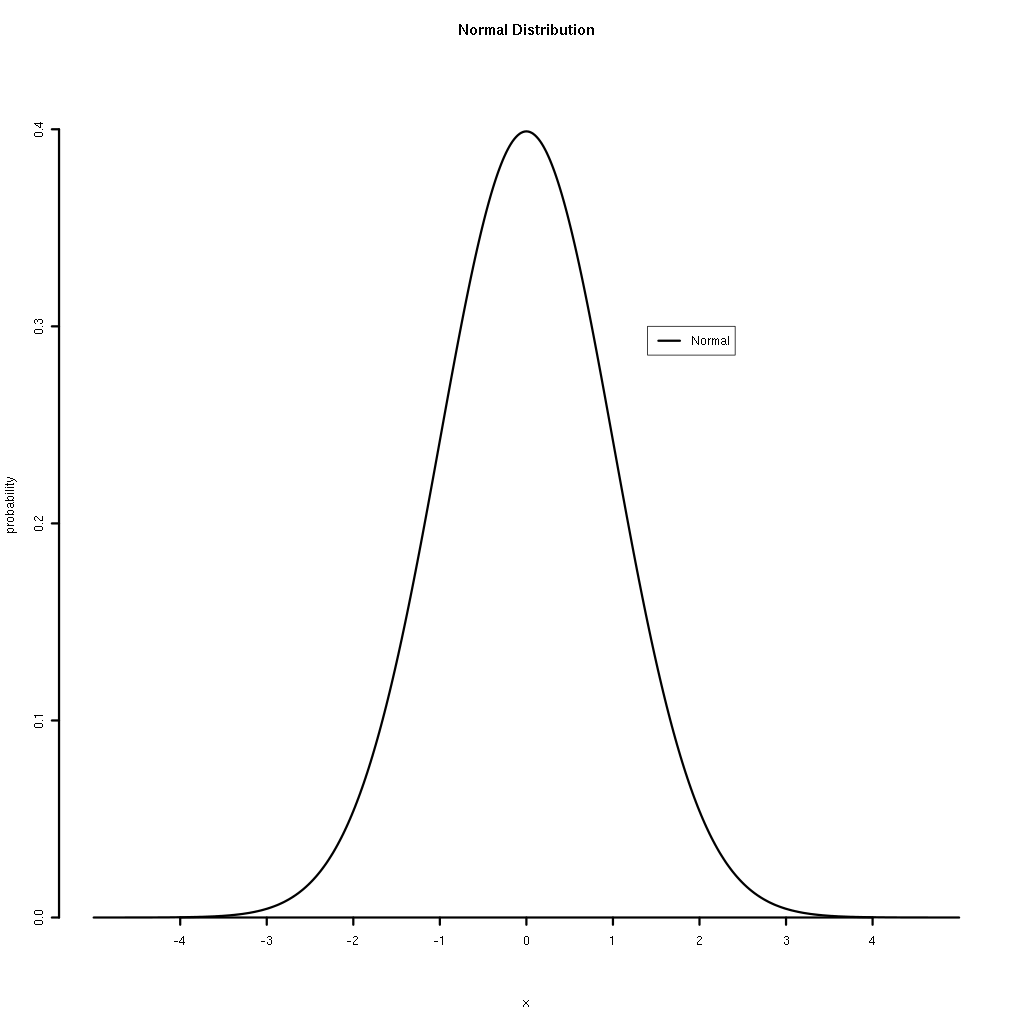
\includegraphics[width=7cm]{img/normalCompare}}
  \only<2-2>{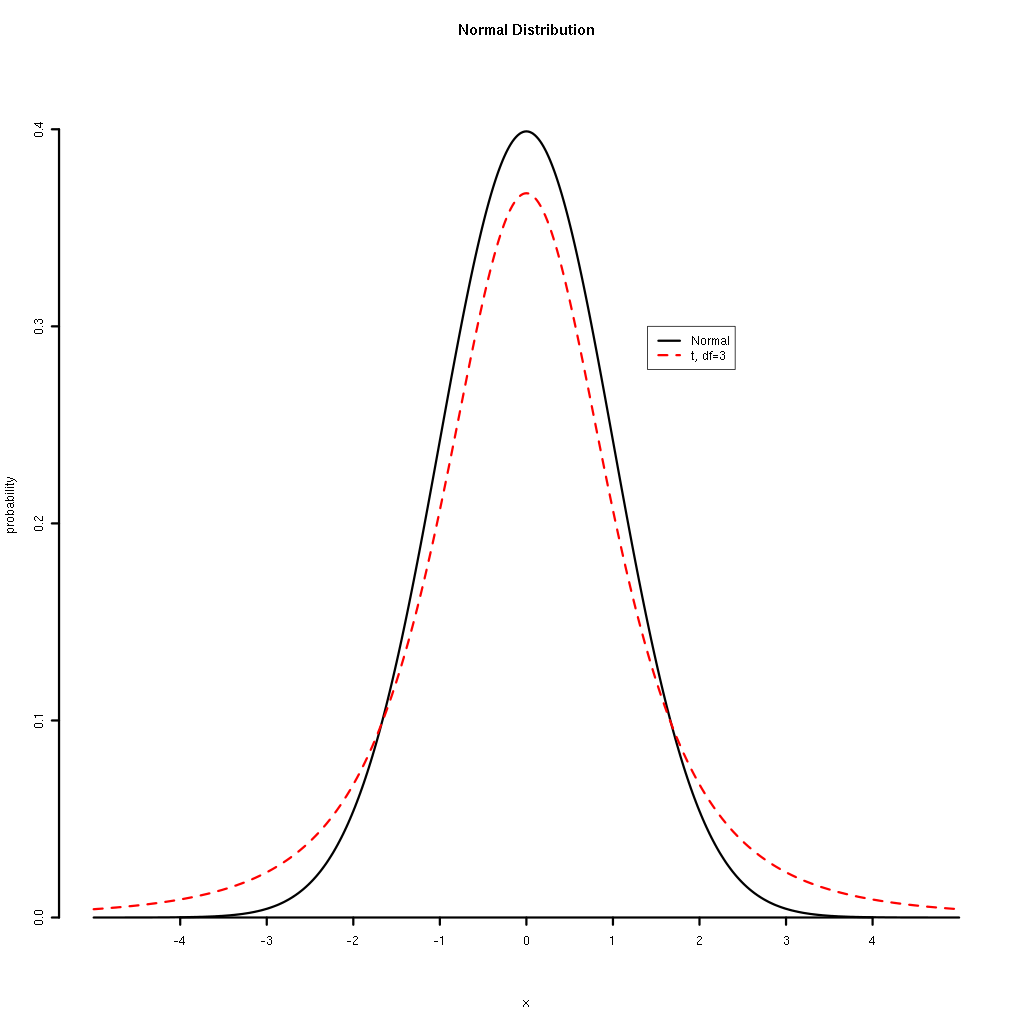
\includegraphics[width=7cm]{img/tDistCompareDF3}}
  \only<3-3>{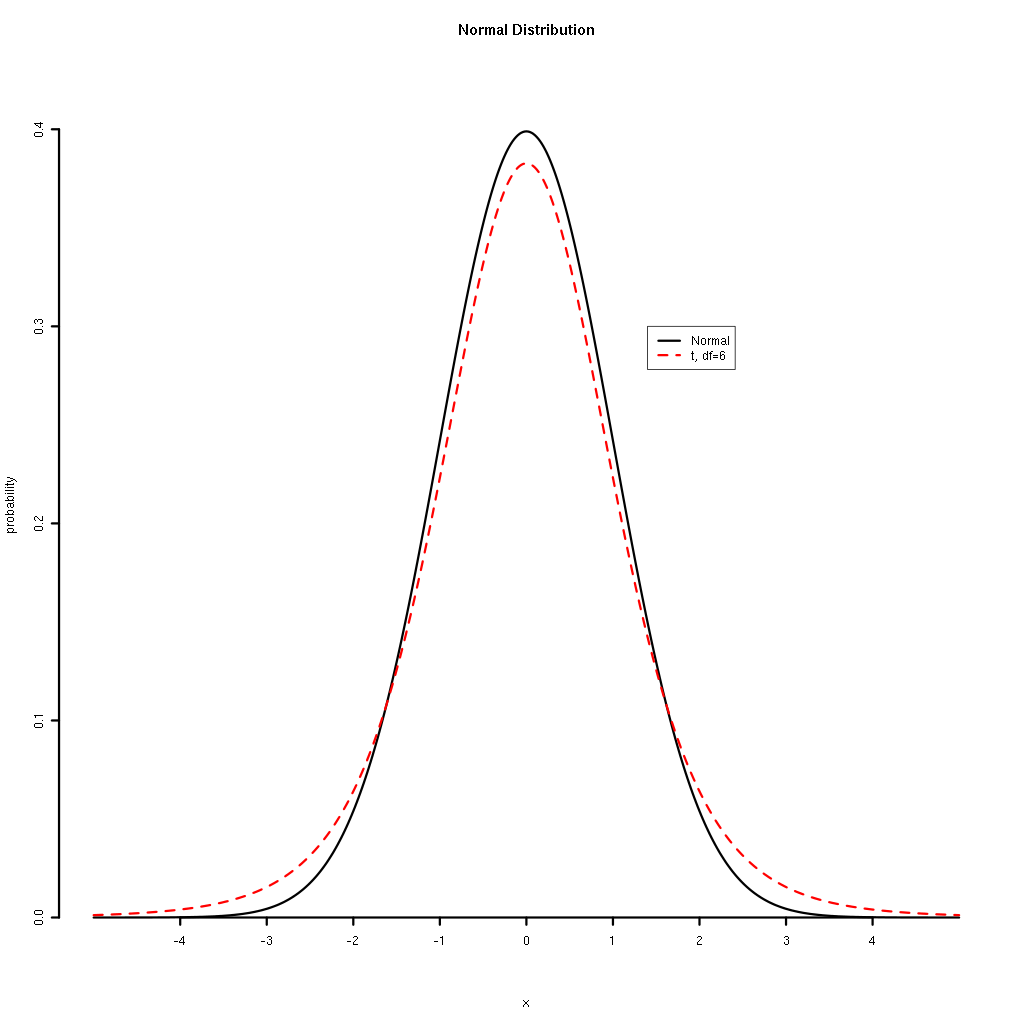
\includegraphics[width=7cm]{img/tDistCompareDF6}}
  \only<4-4>{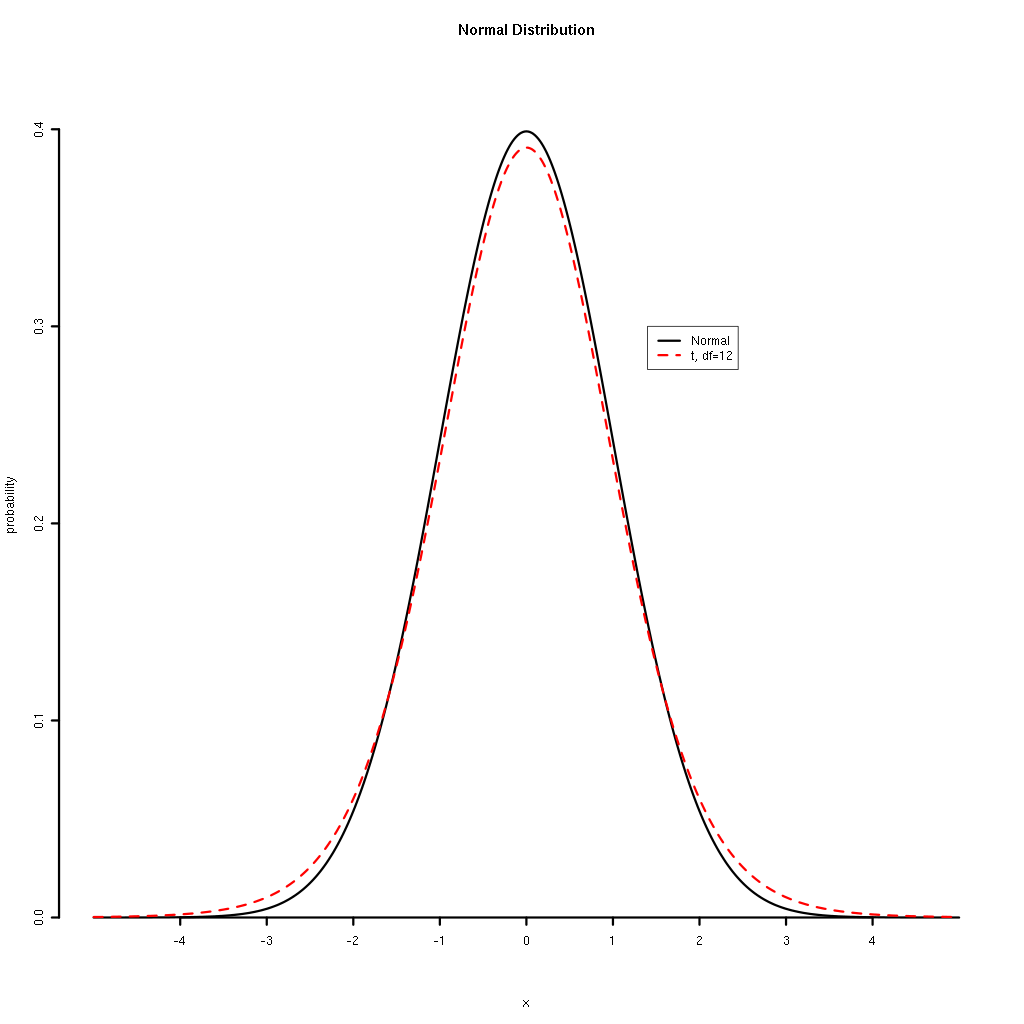
\includegraphics[width=7cm]{img/tDistCompareDF12}}
  \only<5-5>{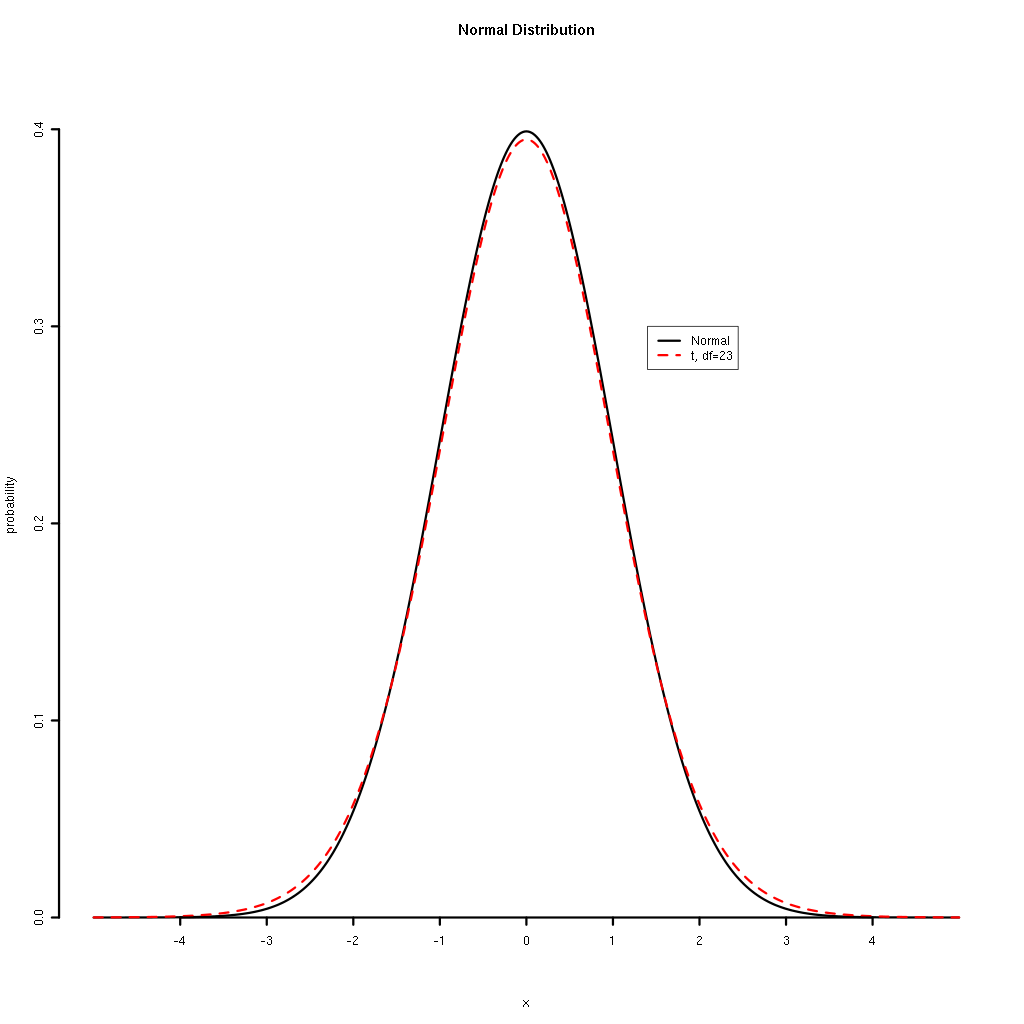
\includegraphics[width=7cm]{img/tDistCompareDF24}}
  

\end{frame}


\begin{frame}
  \frametitle{Comparison}

  \begin{columns}
    \column{0.5\textwidth}
    Normal Distribution:
    \begin{eqnarray*}
      z &  = & \frac{\bar{x}-\mu}{\lp \frac{\sigma}{\sqrt{n}} \rp}.
    \end{eqnarray*}

    \column{0.5\textwidth}
    $t$-Distribution:
    \begin{eqnarray*}
      t &  = & \frac{\bar{x}-\mu}{\lp \frac{s}{\sqrt{n}} \rp}, \\
      df & = & n-1.
    \end{eqnarray*}

  \end{columns}

  \vfill

    \only<2->
    {

      \begin{center}
        The algebra and concepts are exactly the same!

        The only difference is $\sigma$ vs. $s$ and $df=n-1$.
      \end{center}
    }

    \vfill
  

\end{frame}


\begin{frame}{Clicker Quiz}

  \iftoggle{clicker}{%

    \begin{eqnarray*}
      \begin{array}{lrcl}
        H_0: & \mu & = & 45.0 \\
        H_a: & \mu & \neq & 45.0
      \end{array}
    \end{eqnarray*}

    \begin{eqnarray*}
      n & = & 10, \\
      \bar{x} & = & 49.9,\\
      s       & = & 8.0, \\
      \alpha  & = & 0.05.
    \end{eqnarray*}

    \vfill 

    What is the $t$-statistic?

    \begin{tabular}{l@{\hspace{3em}}l@{\hspace{3em}}l@{\hspace{3em}}l}
      A: 0.613  & B: 1.64 & C: 1.94  & D: 1.96 
    \end{tabular}

    \vfill
    \vfill
    \vfill

  }

\end{frame}





% LocalWords:  Clarkson pausesection hideallsubsections lrcl


%\part{}
\lecture{The t-distribution}{t-table}


\title{The $t$-Distribution}
\subtitle{When you only know the sample standard deviation}

\author{Kelly Black}
\institute{Clarkson University}
\date{28 March 2012}

\begin{frame}
  \titlepage
\end{frame}

\begin{frame}
  \frametitle{Outline}
  \tableofcontents[pausesection,hideallsubsections]
\end{frame}


\section{Clicker Quiz}


\begin{frame}{Clicker Quiz}

  \iftoggle{clicker}{%

    \begin{eqnarray*}
      \begin{array}{lrcl}
        H_0: & \mu & = & 350 \\
        H_a: & \mu & \neq & 350
      \end{array}
    \end{eqnarray*}

    \begin{eqnarray*}
      n & = & 13, \\
      \bar{x} & = & 412.4,\\
      s      & = & 75.0, \\
      \alpha & = & 0.01.
    \end{eqnarray*}

    \vfill 

    What is the \textit{critical} $z$-statistic?

    \begin{tabular}{l@{\hspace{3em}}l@{\hspace{3em}}l@{\hspace{3em}}l}
      A: 1.64  & B: 1.94 & C: 2.58  & D: 3.00
    \end{tabular}

    \vfill
    \vfill
    \vfill

  }

\end{frame}


\begin{frame}{Problem!}

  We do not know $\sigma$!

  What do we do?
  
\end{frame}





\section{The $t$-Distribution}


\begin{frame}
  \frametitle{$t$-Distribution}

  \begin{definition}[$t$-Distribution]

    A $t$-distribution is the distribution associated with the expression
    \begin{eqnarray*}
      t &  = & \frac{\bar{x}-\mu}{\lp \frac{s}{\sqrt{n}} \rp}.
    \end{eqnarray*}

    The number of ``\textit{degrees of freedom}'' is $n-1$.
    
  \end{definition}

  Because the distribution depends on $n-1$ means that we need a
  different table for every possible value of $n$. Instead we just
  have a table for the critical values for some values of $n$.
  

\end{frame}



\begin{frame}
  \frametitle{Comparison}

  \begin{columns}
    \column{0.5\textwidth}
    Normal Distribution:
    \begin{eqnarray*}
      z &  = & \frac{\bar{x}-\mu}{\lp \frac{\sigma}{\sqrt{n}} \rp}.
    \end{eqnarray*}

    \column{0.5\textwidth}
    $t$-Distribution:
    \begin{eqnarray*}
      t &  = & \frac{\bar{x}-\mu}{\lp \frac{s}{\sqrt{n}} \rp}, \\
      df & = & n-1.
    \end{eqnarray*}

  \end{columns}

  \vfill

    \only<2->
    {

      \begin{center}
        The algebra and concepts are exactly the same!

        The only difference is $\sigma$ vs. $s$ and $df=n-1$.
      \end{center}
    }

    \vfill
  

\end{frame}



\begin{frame}
  \frametitle{The Table}
  {
\fontencoding{T1}
\fontfamily{pcr}
\fontseries{m}
\fontshape{n}
\fontsize{5pt}{5pt}
\selectfont

\begin{tabular}{l|llllllllll}
 & 0.1&0.05&0.025&0.01&0.005&0.001&0.00005\\ \hline
 1 & 3.078 & 6.314 & 12.706 & 31.821 & 63.657 & 318.309 & 636.619 \\ 
 2 & 1.886 & 2.920 & 4.303 & 6.965 & 9.925 & 22.327 & 31.599 \\ 
 3 & 1.638 & 2.353 & 3.182 & 4.541 & 5.841 & 10.215 & 12.924 \\ 
 4 & 1.533 & 2.132 & 2.776 & 3.747 & 4.604 & 7.173 & 8.610 \\ 
 5 & 1.476 & 2.015 & 2.571 & 3.365 & 4.032 & 5.893 & 6.869 \\ 
[5pt]
 6 & 1.440 & 1.943 & 2.447 & 3.143 & 3.707 & 5.208 & 5.959 \\ 
 7 & 1.415 & 1.895 & 2.365 & 2.998 & 3.499 & 4.785 & 5.408 \\ 
 8 & 1.397 & 1.860 & 2.306 & 2.896 & 3.355 & 4.501 & 5.041 \\ 
 9 & 1.383 & 1.833 & 2.262 & 2.821 & 3.250 & 4.297 & 4.781 \\ 
10 & 1.372 & 1.812 & 2.228 & 2.764 & 3.169 & 4.144 & 4.587 \\ 
[5pt]
11 & 1.363 & 1.796 & 2.201 & 2.718 & 3.106 & 4.025 & 4.437 \\ 
12 & 1.356 & 1.782 & 2.179 & 2.681 & 3.055 & 3.930 & 4.318 \\ 
13 & 1.350 & 1.771 & 2.160 & 2.650 & 3.012 & 3.852 & 4.221 \\ 
14 & 1.345 & 1.761 & 2.145 & 2.624 & 2.977 & 3.787 & 4.140 \\ 
15 & 1.341 & 1.753 & 2.131 & 2.602 & 2.947 & 3.733 & 4.073 \\ 
[5pt]
16 & 1.337 & 1.746 & 2.120 & 2.583 & 2.921 & 3.686 & 4.015 \\ 
17 & 1.333 & 1.740 & 2.110 & 2.567 & 2.898 & 3.646 & 3.965 \\ 
18 & 1.330 & 1.734 & 2.101 & 2.552 & 2.878 & 3.610 & 3.922 \\ 
19 & 1.328 & 1.729 & 2.093 & 2.539 & 2.861 & 3.579 & 3.883 \\ 
20 & 1.325 & 1.725 & 2.086 & 2.528 & 2.845 & 3.552 & 3.850 \\ 
[5pt]
21 & 1.323 & 1.721 & 2.080 & 2.518 & 2.831 & 3.527 & 3.819 \\ 
22 & 1.321 & 1.717 & 2.074 & 2.508 & 2.819 & 3.505 & 3.792 \\ 
23 & 1.319 & 1.714 & 2.069 & 2.500 & 2.807 & 3.485 & 3.768 \\ 
24 & 1.318 & 1.711 & 2.064 & 2.492 & 2.797 & 3.467 & 3.745 \\ 
25 & 1.316 & 1.708 & 2.060 & 2.485 & 2.787 & 3.450 & 3.725 \\ 
[5pt]
26 & 1.315 & 1.706 & 2.056 & 2.479 & 2.779 & 3.435 & 3.707 \\ 
27 & 1.314 & 1.703 & 2.052 & 2.473 & 2.771 & 3.421 & 3.690 \\ 
28 & 1.313 & 1.701 & 2.048 & 2.467 & 2.763 & 3.408 & 3.674 \\ 
29 & 1.311 & 1.699 & 2.045 & 2.462 & 2.756 & 3.396 & 3.659 \\ 
30 & 1.310 & 1.697 & 2.042 & 2.457 & 2.750 & 3.385 & 3.646 \\ 
[5pt]
40 & 1.303 & 1.684 & 2.021 & 2.423 & 2.704 & 3.307 & 3.551 \\ 
50 & 1.299 & 1.676 & 2.009 & 2.403 & 2.678 & 3.261 & 3.496 \\ 
60 & 1.296 & 1.671 & 2.000 & 2.390 & 2.660 & 3.232 & 3.460 \\ 
120 & 1.289 & 1.658 & 1.980 & 2.358 & 2.617 & 3.160 & 3.373 \\ 
$\infty$ & 1.282 & 1.645 & 1.960 & 2.326 & 2.576 & 3.090 & 3.291 
\end{tabular}


}
\end{frame}


\begin{frame}{\small Example: Find $t^*$ value for $p(|t|>t^*)
\approx 0.01$ with 12 degrees of freedom.}
{\tiny First find the row corresponding to $n=12$.}

  {
\fontencoding{T1}
\fontfamily{pcr}
\fontseries{m}
\fontshape{n}
\fontsize{5pt}{5pt}
\selectfont

\begin{tabular}{l|llllllllll}
 & 0.1&0.05&0.025&0.01&0.005&0.001&0.00005\\ \hline
 1 & 3.078 & 6.314 & 12.706 & 31.821 & 63.657 & 318.309 & 636.619 \\ 
 2 & 1.886 & 2.920 & 4.303 & 6.965 & 9.925 & 22.327 & 31.599 \\ 
 3 & 1.638 & 2.353 & 3.182 & 4.541 & 5.841 & 10.215 & 12.924 \\ 
 4 & 1.533 & 2.132 & 2.776 & 3.747 & 4.604 & 7.173 & 8.610 \\ 
 5 & 1.476 & 2.015 & 2.571 & 3.365 & 4.032 & 5.893 & 6.869 \\ 
[5pt]
 6 & 1.440 & 1.943 & 2.447 & 3.143 & 3.707 & 5.208 & 5.959 \\ 
 7 & 1.415 & 1.895 & 2.365 & 2.998 & 3.499 & 4.785 & 5.408 \\ 
 8 & 1.397 & 1.860 & 2.306 & 2.896 & 3.355 & 4.501 & 5.041 \\ 
 9 & 1.383 & 1.833 & 2.262 & 2.821 & 3.250 & 4.297 & 4.781 \\ 
10 & 1.372 & 1.812 & 2.228 & 2.764 & 3.169 & 4.144 & 4.587 \\ 
[5pt]
11 & 1.363 & 1.796 & 2.201 & 2.718 & 3.106 & 4.025 & 4.437 \\ 
\rowcolor{red}12 & 1.356 & 1.782 & 2.179 & 2.681 & 3.055 & 3.930 & 4.318 \\ 
13 & 1.350 & 1.771 & 2.160 & 2.650 & 3.012 & 3.852 & 4.221 \\ 
14 & 1.345 & 1.761 & 2.145 & 2.624 & 2.977 & 3.787 & 4.140 \\ 
15 & 1.341 & 1.753 & 2.131 & 2.602 & 2.947 & 3.733 & 4.073 \\ 
[5pt]
16 & 1.337 & 1.746 & 2.120 & 2.583 & 2.921 & 3.686 & 4.015 \\ 
17 & 1.333 & 1.740 & 2.110 & 2.567 & 2.898 & 3.646 & 3.965 \\ 
18 & 1.330 & 1.734 & 2.101 & 2.552 & 2.878 & 3.610 & 3.922 \\ 
19 & 1.328 & 1.729 & 2.093 & 2.539 & 2.861 & 3.579 & 3.883 \\ 
20 & 1.325 & 1.725 & 2.086 & 2.528 & 2.845 & 3.552 & 3.850 \\ 
[5pt]
21 & 1.323 & 1.721 & 2.080 & 2.518 & 2.831 & 3.527 & 3.819 \\ 
22 & 1.321 & 1.717 & 2.074 & 2.508 & 2.819 & 3.505 & 3.792 \\ 
23 & 1.319 & 1.714 & 2.069 & 2.500 & 2.807 & 3.485 & 3.768 \\ 
24 & 1.318 & 1.711 & 2.064 & 2.492 & 2.797 & 3.467 & 3.745 \\ 
25 & 1.316 & 1.708 & 2.060 & 2.485 & 2.787 & 3.450 & 3.725 \\ 
[5pt]
26 & 1.315 & 1.706 & 2.056 & 2.479 & 2.779 & 3.435 & 3.707 \\ 
27 & 1.314 & 1.703 & 2.052 & 2.473 & 2.771 & 3.421 & 3.690 \\ 
28 & 1.313 & 1.701 & 2.048 & 2.467 & 2.763 & 3.408 & 3.674 \\ 
29 & 1.311 & 1.699 & 2.045 & 2.462 & 2.756 & 3.396 & 3.659 \\ 
30 & 1.310 & 1.697 & 2.042 & 2.457 & 2.750 & 3.385 & 3.646 \\ 
[5pt]
40 & 1.303 & 1.684 & 2.021 & 2.423 & 2.704 & 3.307 & 3.551 \\ 
50 & 1.299 & 1.676 & 2.009 & 2.403 & 2.678 & 3.261 & 3.496 \\ 
60 & 1.296 & 1.671 & 2.000 & 2.390 & 2.660 & 3.232 & 3.460 \\ 
120 & 1.289 & 1.658 & 1.980 & 2.358 & 2.617 & 3.160 & 3.373 \\ 
$\infty$ & 1.282 & 1.645 & 1.960 & 2.326 & 2.576 & 3.090 & 3.291 
\end{tabular}


}



\end{frame}

\begin{frame}
{\small Second find the column corresponding to 0.005. The critical $t$ value is 3.055.}

  {
\fontencoding{T1}
\fontfamily{pcr}
\fontseries{m}
\fontshape{n}
\fontsize{5pt}{5pt}
\selectfont

\begin{tabular}{l|llll>{\columncolor{blue}}llllll}
 & 0.1&0.05&0.025&0.01&0.005&0.001&0.00005\\ \hline
 1 & 3.078 & 6.314 & 12.706 & 31.821 & 63.657 & 318.309 & 636.619 \\ 
 2 & 1.886 & 2.920 & 4.303 & 6.965 & 9.925 & 22.327 & 31.599 \\ 
 3 & 1.638 & 2.353 & 3.182 & 4.541 & 5.841 & 10.215 & 12.924 \\ 
 4 & 1.533 & 2.132 & 2.776 & 3.747 & 4.604 & 7.173 & 8.610 \\ 
 5 & 1.476 & 2.015 & 2.571 & 3.365 & 4.032 & 5.893 & 6.869 \\ 
[5pt]
 6 & 1.440 & 1.943 & 2.447 & 3.143 & 3.707 & 5.208 & 5.959 \\ 
 7 & 1.415 & 1.895 & 2.365 & 2.998 & 3.499 & 4.785 & 5.408 \\ 
 8 & 1.397 & 1.860 & 2.306 & 2.896 & 3.355 & 4.501 & 5.041 \\ 
 9 & 1.383 & 1.833 & 2.262 & 2.821 & 3.250 & 4.297 & 4.781 \\ 
10 & 1.372 & 1.812 & 2.228 & 2.764 & 3.169 & 4.144 & 4.587 \\ 
[5pt]
11 & 1.363 & 1.796 & 2.201 & 2.718 & 3.106 & 4.025 & 4.437 \\ 
\rowcolor{red}12 & 1.356 & 1.782 & 2.179 & 2.681 & 3.055 & 3.930 & 4.318 \\ 
13 & 1.350 & 1.771 & 2.160 & 2.650 & 3.012 & 3.852 & 4.221 \\ 
14 & 1.345 & 1.761 & 2.145 & 2.624 & 2.977 & 3.787 & 4.140 \\ 
15 & 1.341 & 1.753 & 2.131 & 2.602 & 2.947 & 3.733 & 4.073 \\ 
[5pt]
16 & 1.337 & 1.746 & 2.120 & 2.583 & 2.921 & 3.686 & 4.015 \\ 
17 & 1.333 & 1.740 & 2.110 & 2.567 & 2.898 & 3.646 & 3.965 \\ 
18 & 1.330 & 1.734 & 2.101 & 2.552 & 2.878 & 3.610 & 3.922 \\ 
19 & 1.328 & 1.729 & 2.093 & 2.539 & 2.861 & 3.579 & 3.883 \\ 
20 & 1.325 & 1.725 & 2.086 & 2.528 & 2.845 & 3.552 & 3.850 \\ 
[5pt]
21 & 1.323 & 1.721 & 2.080 & 2.518 & 2.831 & 3.527 & 3.819 \\ 
22 & 1.321 & 1.717 & 2.074 & 2.508 & 2.819 & 3.505 & 3.792 \\ 
23 & 1.319 & 1.714 & 2.069 & 2.500 & 2.807 & 3.485 & 3.768 \\ 
24 & 1.318 & 1.711 & 2.064 & 2.492 & 2.797 & 3.467 & 3.745 \\ 
25 & 1.316 & 1.708 & 2.060 & 2.485 & 2.787 & 3.450 & 3.725 \\ 
[5pt]
26 & 1.315 & 1.706 & 2.056 & 2.479 & 2.779 & 3.435 & 3.707 \\ 
27 & 1.314 & 1.703 & 2.052 & 2.473 & 2.771 & 3.421 & 3.690 \\ 
28 & 1.313 & 1.701 & 2.048 & 2.467 & 2.763 & 3.408 & 3.674 \\ 
29 & 1.311 & 1.699 & 2.045 & 2.462 & 2.756 & 3.396 & 3.659 \\ 
30 & 1.310 & 1.697 & 2.042 & 2.457 & 2.750 & 3.385 & 3.646 \\ 
[5pt]
40 & 1.303 & 1.684 & 2.021 & 2.423 & 2.704 & 3.307 & 3.551 \\ 
50 & 1.299 & 1.676 & 2.009 & 2.403 & 2.678 & 3.261 & 3.496 \\ 
60 & 1.296 & 1.671 & 2.000 & 2.390 & 2.660 & 3.232 & 3.460 \\ 
120 & 1.289 & 1.658 & 1.980 & 2.358 & 2.617 & 3.160 & 3.373 \\ 
$\infty$ & 1.282 & 1.645 & 1.960 & 2.326 & 2.576 & 3.090 & 3.291 
\end{tabular}


}

\end{frame}


\begin{frame}{Our First Example}


    \begin{eqnarray*}
      \begin{array}{lrcl}
        H_0: & \mu & = & 350 \\
        H_a: & \mu & \neq & 350
      \end{array}
    \end{eqnarray*}

    \begin{eqnarray*}
      n & = & 13, \\
      \bar{x} & = & 412.4,\\
      s      & = & 75.0, \\
      \alpha & = & 0.01.
    \end{eqnarray*}

    \vfill 

    The \textit{critical} $t$-statistic is 
    \begin{eqnarray*}
      t^* & = & 3.055.
    \end{eqnarray*}

    The $t$-statistic from the data is
    \begin{eqnarray*}
      t & = & \frac{412.4-350}{\frac{75}{\sqrt{13}}}, \\
        & \approx & 3.00.
    \end{eqnarray*}



\end{frame}

\begin{frame}{Result}

  We \textbf{do not} have sufficient evidence to reject $H_0$ at the
  1\% significance level using a $t$-distribution with thirteen
  samples and a standard deviation of 75.
  
\end{frame}


\begin{frame}{Let's Change Our First Example}


    \begin{eqnarray*}
      \begin{array}{lrcl}
        H_0: & \mu & = & 350 \\
        H_a: & \mu & \neq & 350
      \end{array}
    \end{eqnarray*}

    \begin{eqnarray*}
      n & = & 13, \\
      \bar{x} & = & 412.4,\\
      s      & = & 75.0, \\
      \alpha & = & 0.05.
    \end{eqnarray*}

    \vfill 

    The $t$-statistic from the data is
    \begin{eqnarray*}
      t & = & \frac{412.4-350}{\frac{75}{\sqrt{13}}}, \\
        & \approx & 3.00.
    \end{eqnarray*}


    What is the critical $t$-statistic?

\end{frame}



\begin{frame}{\small Example: Find $t^*$ value for $p(|t|>t^*)
\approx 0.01$ with 12 degrees of freedom.}
  
{\small First find the row corresponding to $n=12$.}

  {
\fontencoding{T1}
\fontfamily{pcr}
\fontseries{m}
\fontshape{n}
\fontsize{5pt}{5pt}
\selectfont

\begin{tabular}{l|llllllllll}
 & 0.1&0.05&0.025&0.01&0.005&0.001&0.00005\\ \hline
 1 & 3.078 & 6.314 & 12.706 & 31.821 & 63.657 & 318.309 & 636.619 \\ 
 2 & 1.886 & 2.920 & 4.303 & 6.965 & 9.925 & 22.327 & 31.599 \\ 
 3 & 1.638 & 2.353 & 3.182 & 4.541 & 5.841 & 10.215 & 12.924 \\ 
 4 & 1.533 & 2.132 & 2.776 & 3.747 & 4.604 & 7.173 & 8.610 \\ 
 5 & 1.476 & 2.015 & 2.571 & 3.365 & 4.032 & 5.893 & 6.869 \\ 
[5pt]
 6 & 1.440 & 1.943 & 2.447 & 3.143 & 3.707 & 5.208 & 5.959 \\ 
 7 & 1.415 & 1.895 & 2.365 & 2.998 & 3.499 & 4.785 & 5.408 \\ 
 8 & 1.397 & 1.860 & 2.306 & 2.896 & 3.355 & 4.501 & 5.041 \\ 
 9 & 1.383 & 1.833 & 2.262 & 2.821 & 3.250 & 4.297 & 4.781 \\ 
10 & 1.372 & 1.812 & 2.228 & 2.764 & 3.169 & 4.144 & 4.587 \\ 
[5pt]
11 & 1.363 & 1.796 & 2.201 & 2.718 & 3.106 & 4.025 & 4.437 \\ 
\rowcolor{red}12 & 1.356 & 1.782 & 2.179 & 2.681 & 3.055 & 3.930 & 4.318 \\ 
13 & 1.350 & 1.771 & 2.160 & 2.650 & 3.012 & 3.852 & 4.221 \\ 
14 & 1.345 & 1.761 & 2.145 & 2.624 & 2.977 & 3.787 & 4.140 \\ 
15 & 1.341 & 1.753 & 2.131 & 2.602 & 2.947 & 3.733 & 4.073 \\ 
[5pt]
16 & 1.337 & 1.746 & 2.120 & 2.583 & 2.921 & 3.686 & 4.015 \\ 
17 & 1.333 & 1.740 & 2.110 & 2.567 & 2.898 & 3.646 & 3.965 \\ 
18 & 1.330 & 1.734 & 2.101 & 2.552 & 2.878 & 3.610 & 3.922 \\ 
19 & 1.328 & 1.729 & 2.093 & 2.539 & 2.861 & 3.579 & 3.883 \\ 
20 & 1.325 & 1.725 & 2.086 & 2.528 & 2.845 & 3.552 & 3.850 \\ 
[5pt]
21 & 1.323 & 1.721 & 2.080 & 2.518 & 2.831 & 3.527 & 3.819 \\ 
22 & 1.321 & 1.717 & 2.074 & 2.508 & 2.819 & 3.505 & 3.792 \\ 
23 & 1.319 & 1.714 & 2.069 & 2.500 & 2.807 & 3.485 & 3.768 \\ 
24 & 1.318 & 1.711 & 2.064 & 2.492 & 2.797 & 3.467 & 3.745 \\ 
25 & 1.316 & 1.708 & 2.060 & 2.485 & 2.787 & 3.450 & 3.725 \\ 
[5pt]
26 & 1.315 & 1.706 & 2.056 & 2.479 & 2.779 & 3.435 & 3.707 \\ 
27 & 1.314 & 1.703 & 2.052 & 2.473 & 2.771 & 3.421 & 3.690 \\ 
28 & 1.313 & 1.701 & 2.048 & 2.467 & 2.763 & 3.408 & 3.674 \\ 
29 & 1.311 & 1.699 & 2.045 & 2.462 & 2.756 & 3.396 & 3.659 \\ 
30 & 1.310 & 1.697 & 2.042 & 2.457 & 2.750 & 3.385 & 3.646 \\ 
[5pt]
40 & 1.303 & 1.684 & 2.021 & 2.423 & 2.704 & 3.307 & 3.551 \\ 
50 & 1.299 & 1.676 & 2.009 & 2.403 & 2.678 & 3.261 & 3.496 \\ 
60 & 1.296 & 1.671 & 2.000 & 2.390 & 2.660 & 3.232 & 3.460 \\ 
120 & 1.289 & 1.658 & 1.980 & 2.358 & 2.617 & 3.160 & 3.373 \\ 
$\infty$ & 1.282 & 1.645 & 1.960 & 2.326 & 2.576 & 3.090 & 3.291 
\end{tabular}


}



\end{frame}

\begin{frame}
{\small Second find the column corresponding to 0.005. The critical $t$ value is 2.179.}

  {
\fontencoding{T1}
\fontfamily{pcr}
\fontseries{m}
\fontshape{n}
\fontsize{5pt}{5pt}
\selectfont

\begin{tabular}{l|ll>{\columncolor{blue}}llllllll}
 & 0.1&0.05&0.025&0.01&0.005&0.001&0.00005\\ \hline
 1 & 3.078 & 6.314 & 12.706 & 31.821 & 63.657 & 318.309 & 636.619 \\ 
 2 & 1.886 & 2.920 & 4.303 & 6.965 & 9.925 & 22.327 & 31.599 \\ 
 3 & 1.638 & 2.353 & 3.182 & 4.541 & 5.841 & 10.215 & 12.924 \\ 
 4 & 1.533 & 2.132 & 2.776 & 3.747 & 4.604 & 7.173 & 8.610 \\ 
 5 & 1.476 & 2.015 & 2.571 & 3.365 & 4.032 & 5.893 & 6.869 \\ 
[5pt]
 6 & 1.440 & 1.943 & 2.447 & 3.143 & 3.707 & 5.208 & 5.959 \\ 
 7 & 1.415 & 1.895 & 2.365 & 2.998 & 3.499 & 4.785 & 5.408 \\ 
 8 & 1.397 & 1.860 & 2.306 & 2.896 & 3.355 & 4.501 & 5.041 \\ 
 9 & 1.383 & 1.833 & 2.262 & 2.821 & 3.250 & 4.297 & 4.781 \\ 
10 & 1.372 & 1.812 & 2.228 & 2.764 & 3.169 & 4.144 & 4.587 \\ 
[5pt]
11 & 1.363 & 1.796 & 2.201 & 2.718 & 3.106 & 4.025 & 4.437 \\ 
\rowcolor{red}12 & 1.356 & 1.782 & 2.179 & 2.681 & 3.055 & 3.930 & 4.318 \\ 
13 & 1.350 & 1.771 & 2.160 & 2.650 & 3.012 & 3.852 & 4.221 \\ 
14 & 1.345 & 1.761 & 2.145 & 2.624 & 2.977 & 3.787 & 4.140 \\ 
15 & 1.341 & 1.753 & 2.131 & 2.602 & 2.947 & 3.733 & 4.073 \\ 
[5pt]
16 & 1.337 & 1.746 & 2.120 & 2.583 & 2.921 & 3.686 & 4.015 \\ 
17 & 1.333 & 1.740 & 2.110 & 2.567 & 2.898 & 3.646 & 3.965 \\ 
18 & 1.330 & 1.734 & 2.101 & 2.552 & 2.878 & 3.610 & 3.922 \\ 
19 & 1.328 & 1.729 & 2.093 & 2.539 & 2.861 & 3.579 & 3.883 \\ 
20 & 1.325 & 1.725 & 2.086 & 2.528 & 2.845 & 3.552 & 3.850 \\ 
[5pt]
21 & 1.323 & 1.721 & 2.080 & 2.518 & 2.831 & 3.527 & 3.819 \\ 
22 & 1.321 & 1.717 & 2.074 & 2.508 & 2.819 & 3.505 & 3.792 \\ 
23 & 1.319 & 1.714 & 2.069 & 2.500 & 2.807 & 3.485 & 3.768 \\ 
24 & 1.318 & 1.711 & 2.064 & 2.492 & 2.797 & 3.467 & 3.745 \\ 
25 & 1.316 & 1.708 & 2.060 & 2.485 & 2.787 & 3.450 & 3.725 \\ 
[5pt]
26 & 1.315 & 1.706 & 2.056 & 2.479 & 2.779 & 3.435 & 3.707 \\ 
27 & 1.314 & 1.703 & 2.052 & 2.473 & 2.771 & 3.421 & 3.690 \\ 
28 & 1.313 & 1.701 & 2.048 & 2.467 & 2.763 & 3.408 & 3.674 \\ 
29 & 1.311 & 1.699 & 2.045 & 2.462 & 2.756 & 3.396 & 3.659 \\ 
30 & 1.310 & 1.697 & 2.042 & 2.457 & 2.750 & 3.385 & 3.646 \\ 
[5pt]
40 & 1.303 & 1.684 & 2.021 & 2.423 & 2.704 & 3.307 & 3.551 \\ 
50 & 1.299 & 1.676 & 2.009 & 2.403 & 2.678 & 3.261 & 3.496 \\ 
60 & 1.296 & 1.671 & 2.000 & 2.390 & 2.660 & 3.232 & 3.460 \\ 
120 & 1.289 & 1.658 & 1.980 & 2.358 & 2.617 & 3.160 & 3.373 \\ 
$\infty$ & 1.282 & 1.645 & 1.960 & 2.326 & 2.576 & 3.090 & 3.291 
\end{tabular}


}

\end{frame}



\begin{frame}{Let's Change Our First Example}


    \begin{eqnarray*}
      \begin{array}{lrcl}
        H_0: & \mu & = & 350 \\
        H_a: & \mu & \neq & 350
      \end{array}
    \end{eqnarray*}

    \begin{eqnarray*}
      n & = & 13, \\
      \bar{x} & = & 412.4,\\
      s      & = & 75.0, \\
      \alpha & = & 0.05.
    \end{eqnarray*}

    \vfill 

    The $t$-statistic from the data is
    \begin{eqnarray*}
      t & = & \frac{412.4-350}{\frac{75}{\sqrt{13}}}, \\
        & \approx & 3.00.
    \end{eqnarray*}


    \begin{eqnarray*}
      t^* & \approx & 2.179.
    \end{eqnarray*}

\end{frame}


\begin{frame}{Result}

  We have sufficient evidence to reject $H_0$ at the 1\% significance
  level using a $t$-distribution with thirteen samples and a standard
  deviation of 75.
  
\end{frame}




\begin{frame}{Clicker Quiz}

  \iftoggle{clicker}{%

    \begin{eqnarray*}
      \begin{array}{lrcl}
        H_0: & \mu & = &  10 \\
        H_a: & \mu & \neq & 10
      \end{array}
    \end{eqnarray*}

    \begin{eqnarray*}
      n & = & 17, \\
      \bar{x} & = & 8.5,\\
      s      & = & 3.0, \\
      \alpha & = & 0.05.
    \end{eqnarray*}

    \vfill 


    \begin{tabular}{l@{\hspace{3em}}l@{\hspace{3em}}l@{\hspace{3em}}l}
      A: Reject $H_0$  & B: Cannot reject $H_0$ 
    \end{tabular}

    \vfill
    \vfill
    \vfill

  }

\end{frame}





% LocalWords:  Clarkson pausesection hideallsubsections



\lecture{Inference and Proportions}{inference-and-proportions}
\part{Inference and Proportions}

\title{Inference and Proportions}
\subtitle{Our Old Friend the Binomial Distribution}

\author{Kelly Black}
\institute{Clarkson University}
\date{2 April 2012}

\begin{frame}
  \titlepage
\end{frame}

\begin{frame}
  \frametitle{Outline}
  \tableofcontents[pausesection,hideallsubsections,part=1]
\end{frame}



\section{Clicker Quiz}


\begin{frame}{Clicker Quiz}

  \iftoggle{clicker}{%

    \begin{eqnarray*}
      \begin{array}{lrcl}
        H_0: & \mu & = & 50.0 \\
        H_a: & \mu & > & 50.0
      \end{array}
    \end{eqnarray*}

    \begin{eqnarray*}
      n & = & 12, \\
      \bar{x} & = & 56.3,\\
      s       & = & 12.0, \\
      \alpha  & = & 0.05.
    \end{eqnarray*}

    \vfill 


    \begin{tabular}{l@{\hspace{3em}}l@{\hspace{3em}}l@{\hspace{3em}}l}
      A: Reject $H_o$  & B: Do not reject $H_o$
    \end{tabular}

    \vfill
    \vfill
    \vfill

  }

\end{frame}





\section{Proportions}

\begin{frame}
  \frametitle{Example}

  You ask thirty people at random if they will vote for your
  candidate. Seventeen say yes. What is the confidence interval for
  the percentage of people who support your candidate? Use a 95\%
  confidence level.

  \vfill

  \only<2->
  {
    Let $X$ be a binomial distribution with a probability $p$ of
    success and $n$ trials.
  }

  \vfill

  \only<3->
  {
    If $n\cdot p \geq 5$ \textbf{and} $n\cdot (1-p) \geq 5$ then $X$
    is approximately normally distributed with mean $n\cdot p$ and
    standard deviation $\sqrt{p(1-p)n}$.
  }

\end{frame}


\begin{frame}
  \frametitle{Not What We Have!}

  We are asked about the \textit{proportion} not the total number who
  say ``yes.''

  \vfill

  \begin{definition}[The sample proportion]

    We take a sample from $n$ trials. Each trial has probability $p$
    of ``success.'' We count the total number of successes from the
    $n$ trials.  The sample proportion is defined to be
    \begin{eqnarray*}
      \hat{p} & = & \frac{\mathrm{number~of~successes}}{n}.
    \end{eqnarray*}
    
  \end{definition}



\end{frame}

\begin{frame}
  \frametitle{The sample proportion}

  The sample proportion has a mean of $p$, and a standard deviation of
  $\sqrt{\frac{p(1-p)}{n}}$.

  \vfill

  \only<2->
  {

    If $p\cdot n \geq 5$ \textbf{and} $(1-p)\cdot n \geq 5$
    \textbf{and} $n\geq 20$ then $\hat{p}$ is approximately normally
    distributed with mean $p$ and standard deviation
    $\sqrt{\frac{p(1-p)}{n}}$.

  }

  \vfill

  \only<3->
  {
    If this is the case we have
    \begin{eqnarray*}
      z & = & \frac{\hat{p}-p}{\sqrt{\frac{p(1-p)}{n}}}.
    \end{eqnarray*}
  }

  \vfill

  \only<4->
  {
    Problem: We do not know $p$. That is okay just use $\hat{p}$ or
    assume $p=\frac{1}{2}$ for the ``worst case scenario.''
  }


\end{frame}

\begin{frame}
  \frametitle{Example}

  You ask thirty people at random if they will vote for your
  candidate. Seventeen say yes. What is the confidence interval for
  the percentage of people who support your candidate? Use a 95\%
  confidence level.

  \vfill

  \only<2->
  {

    The 95\% confidence interval for the proportion is between .389
    and .745 assuming a normal approximation to the sample proportion.

  }

\end{frame}


\begin{frame}{Clicker Quiz}

  \iftoggle{clicker}{%

    A new drug is tested on one-thousand and eighteen people. Of those
    taking the drug, seven-hundred and fifteen show adequate
    improvement. Find the 95\% confidence interval for the proportion
    of people who will see an adequate improvement.

    \vfill 


    \begin{tabular}{l@{\hspace{3em}}l@{\hspace{3em}}l@{\hspace{3em}}l}
      A: .67 to .73  & B: .66 to .75 & C: -.19 to 1.60
    \end{tabular}

    \vfill
    \vfill
    \vfill

  }

\end{frame}


\begin{frame}{In a nutshell}

  \begin{eqnarray*}
    z & = & \frac{\mathrm{error}}{\sqrt{\frac{p(1-p)}{n}}},
  \end{eqnarray*}

  \begin{tabular}{ll}
    Given $\alpha$, $\hat{p}$, $n$ & Find the error. (*) \\
    Given $\alpha$, error, $n$ & Find $\hat{p}$. \\
    Given $\alpha$, error & Find $n$. (*) \\
  \end{tabular}
  
\end{frame}

\begin{frame}{Clicker Quiz}

  \iftoggle{clicker}{%

    i want to conduct a poll so the probability that the true
    proportion will be in a 95\% confidence interval with an error of
    $\pm 0.03$. How many people should I poll?

    \vfill 


    \begin{tabular}{l@{\hspace{3em}}l@{\hspace{3em}}l@{\hspace{3em}}l}
      A: 33  & B: 267 & C: 1068 & D: 2014
    \end{tabular}

    \vfill
    \vfill
    \vfill

  }

\end{frame}


\begin{frame}{Clicker Quiz}

  \iftoggle{clicker}{%

    An advertisement includes a claim that ten percent of all people
    use a particular brand of toilet paper. I think that it should be
    more than that. I poll nine-hundred and fifty-six people and ask
    them if they use this brand of toilet paper. One-hundred and ten
    say yes. Is the claim true? (Use a five percent significant
    level.)

    \vfill 


    \begin{tabular}{l@{\hspace{3em}}l@{\hspace{3em}}l@{\hspace{3em}}l}
      A: Reject $H_o$.  & Do not reject $H_0$.
    \end{tabular}

    \vfill
    \vfill
    \vfill

  }

\end{frame}


% LocalWords:  Clarkson pausesection hideallsubsections


%\part{}
\lecture{Dependent Populations}{dependent-populations}


\title{Two Populations}
\subtitle{Dependent Populations}

\author{Kelly Black}
\institute{Clarkson University}
\date{6 April 2012}

\begin{frame}
  \titlepage
\end{frame}

\begin{frame}
  \frametitle{Outline}
  \tableofcontents[pausesection,hideallsubsections]
\end{frame}

\section{Clicker Quiz}

\begin{frame}{Clicker Quiz}

  \iftoggle{clicker}{%

    An advertisement includes a claim that ten percent of all people
    use a particular brand of toilet paper. I think that it should be
    more than that. I poll nine-hundred and fifty-six people and ask
    them if they use this brand of toilet paper. One-hundred and ten
    say yes. Is the claim true? (Use a five percent significant
    level.)

    \vfill 


    \begin{tabular}{l@{\hspace{3em}}l@{\hspace{3em}}l@{\hspace{3em}}l}
      A: Reject $H_o$.  & Do not reject $H_0$.
    \end{tabular}

    \vfill
    \vfill
    \vfill

  }

\end{frame}


\begin{frame}
  \frametitle{Comparison}

  \begin{columns}
    \column{0.33\textwidth}
    Normal Distribution:
    \begin{eqnarray*}
      z &  = & \frac{\bar{x}-\mu}{\lp \frac{\sigma}{\sqrt{n}} \rp}.
    \end{eqnarray*}

    \column{0.33\textwidth}
    $t$-Distribution:
    \begin{eqnarray*}
      t &  = & \frac{\bar{x}-\mu}{\lp \frac{s}{\sqrt{n}} \rp}, \\
      df & = & n-1.
    \end{eqnarray*}

    \column{0.33\textwidth}
    Proportions:
    \begin{eqnarray*}
      z & = & \frac{\hat{p}-p}{\sqrt{\frac{p(1-p)}{n}}},
    \end{eqnarray*}


  \end{columns}

  \vfill

    \only<2->
    {
      \begin{center}
        The algebra and concepts are exactly the same!
      \end{center}
    }

    \vfill
  

\end{frame}


\section{Multiple Samples}


\begin{frame}
  \frametitle{Example}

  I pick a random sample of one-hundred stocks and calculate their
  predicted values in one year using a model. I then pick a random
  sample of one-hundred and ten stocks and get their predicted values
  in one year using a different model. Is there a difference in the
  mean stock price after one year between the two models?

  \uncover<2->
  {
    \begin{columns}
      \column{.5\textwidth}
      \begin{tabular}{l}
        Group 1 \\ \hline
        $N_1=100$, \\
        $\bar{x}$, \\
        $s_x$
      \end{tabular}

      \column{.5\textwidth}
      \begin{tabular}{l}
        Group 2 \\ \hline
        $N_2=110$, \\
        $\bar{y}$, \\
        $s_y$
      \end{tabular}

    \end{columns}
  }

  \uncover<3->
  {
    Independent Samples!
  }

  \hfill

\end{frame}


\begin{frame}
  \frametitle{Example}

  I pick a random sample of one-hundred stocks and calculate their
  predicted values in one year using a model. I then wait a year and
  get their actual values. Is there a difference in the mean predicted
  prices and the actual prices?

  \uncover<2->
  {
    \begin{columns}
      \column{.5\textwidth}
      \begin{tabular}{l}
        Group 1 Predicted \\ \hline
        $N=100$, \\
        Predicted Price
      \end{tabular}

      \column{.5\textwidth}
      \begin{tabular}{l}
        Group 1 Actual \\ \hline
        $N=100$, \\
        Actual Price
      \end{tabular}

    \end{columns}
  }

  \uncover<3->
  {
    Dependent Samples!
  }

  \hfill

\end{frame}



\begin{frame}
  \frametitle{Great, more stuff?}
  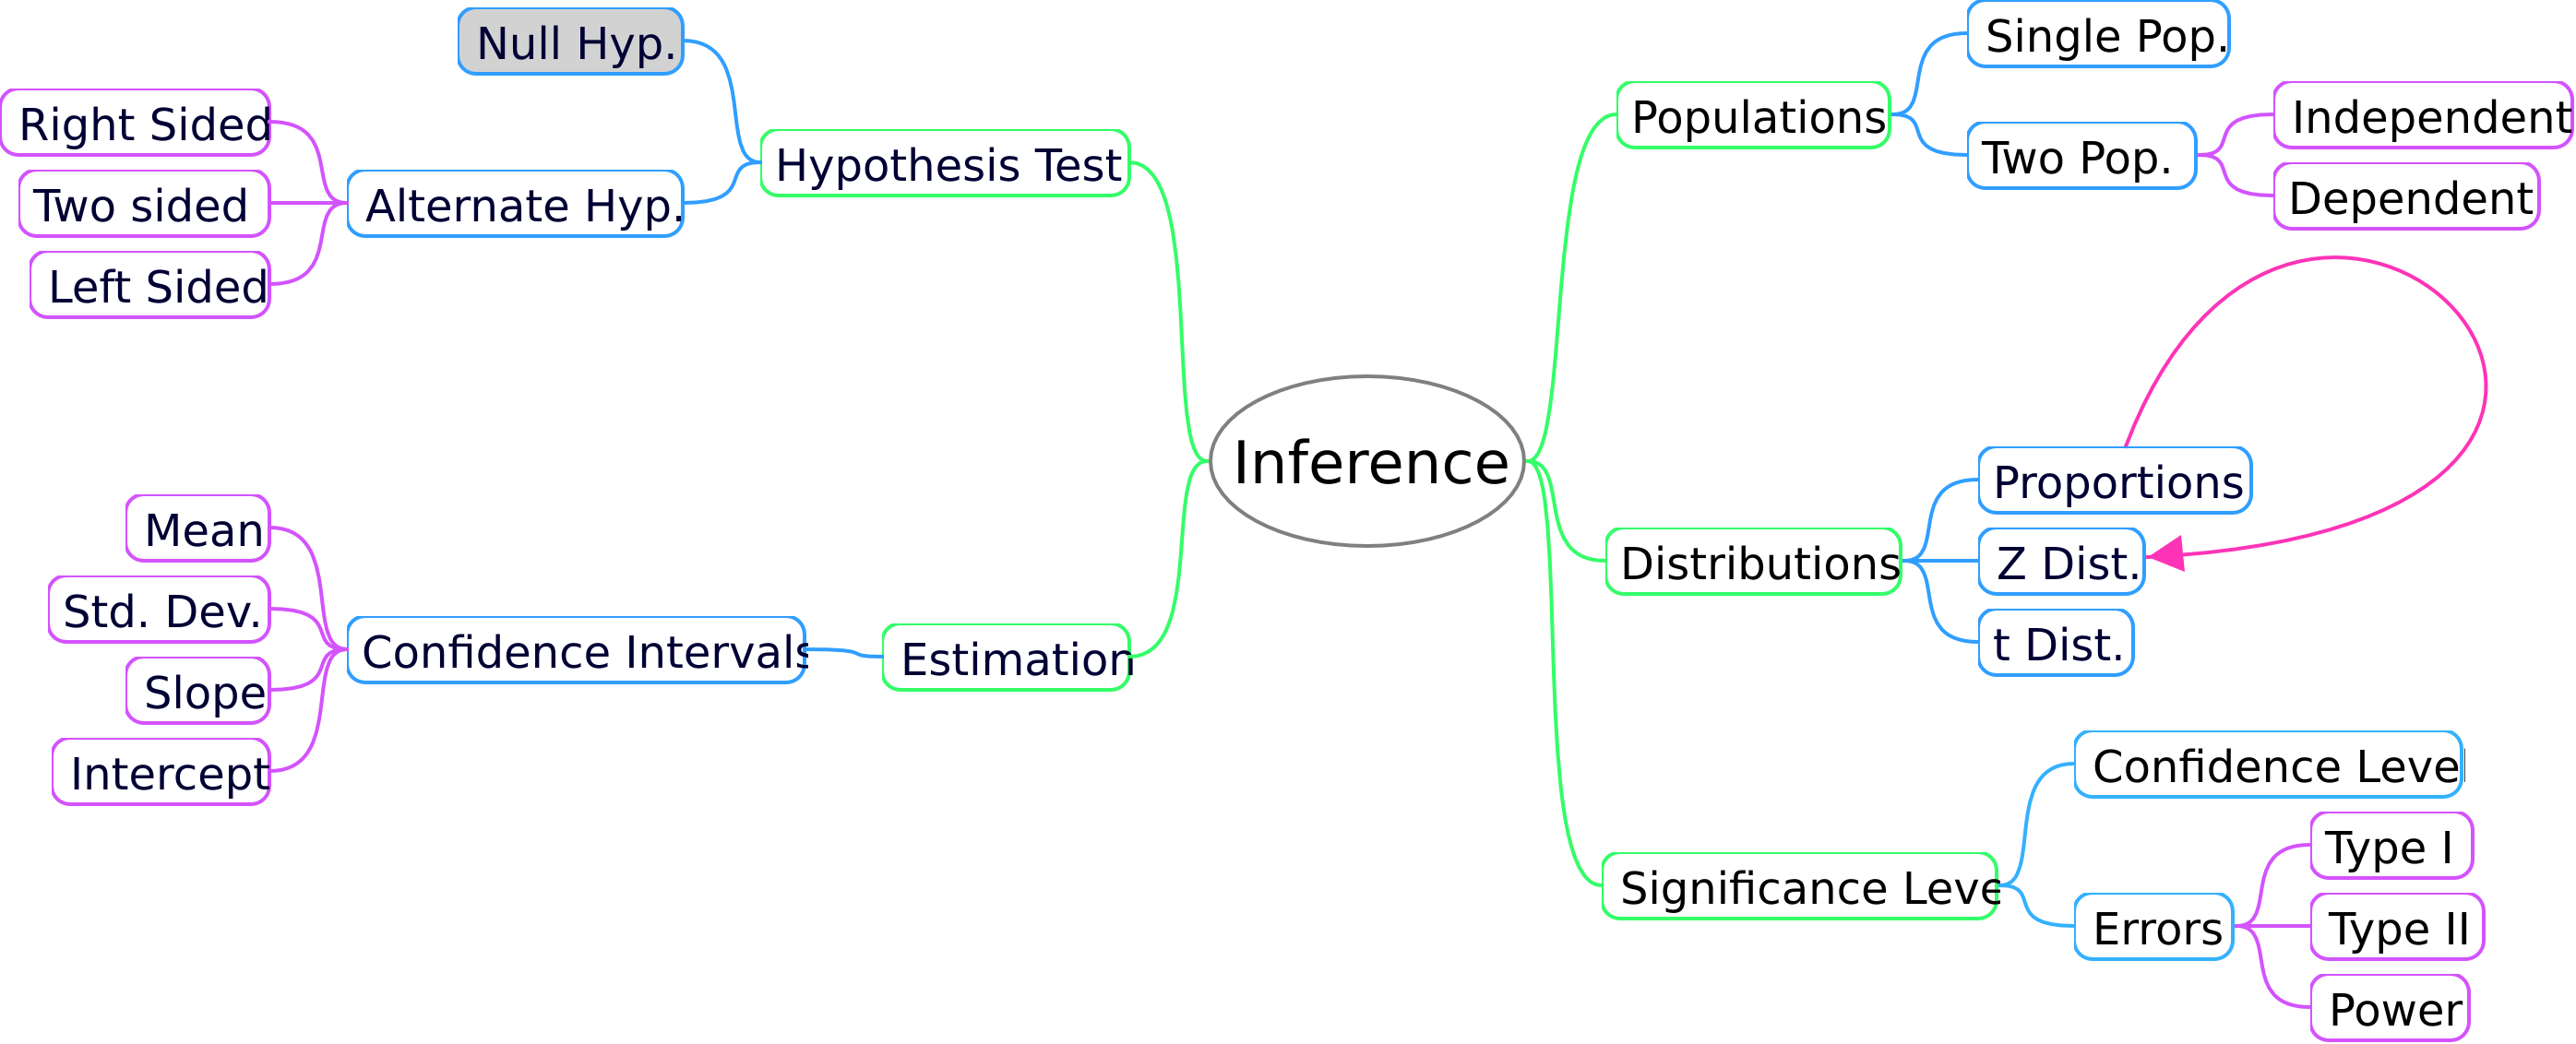
\includegraphics[width=8.5cm]{img/inference}
\end{frame}


\section{Dependent Populations}

\begin{frame}
  \frametitle{Dependent Populations}
% $\RightArrow$ {\onslide<2->}

  \only<3->{We can calculate a set of \textit{paired differences.}}
  \begin{tabular}{l<{\onslide<2->}l<{\onslide<3->}ll<{\onslide}l}
    Before & After & & Difference \\
    $x_1$ & $y_1$ & $\Rightarrow$ & $x_1-y_1$ \\
    $x_2$ & $y_2$ & $\Rightarrow$ & $x_2-y_2$ \\
    $x_3$ & $y_3$ & $\Rightarrow$ & $x_3-y_3$ \\
    $x_4$ & $y_4$ & $\Rightarrow$ & $x_4-y_4$ \\
    $\vdots$ & $\vdots$ & & $\vdots$ \\
    $x_n$ & $y_n$ & $\Rightarrow$ & $x_n-y_n$ \\
  \end{tabular}

\end{frame}


\begin{frame}{Another View}

  You have a set of ``before'' data:
  \begin{eqnarray*}
    \begin{array}{lllll}
      x_1 & x_2 & x_3 & \cdots & x_n
    \end{array}
  \end{eqnarray*}

  \only<2->
  {
    You have a set of ``after'' data:
    \begin{eqnarray*}
      \begin{array}{lllll}
        y_1 & y_2 & y_3 & \cdots & y_n
      \end{array}
    \end{eqnarray*}
  }

  \only<3->
  {
    You calculate a difference:
    \begin{eqnarray*}
      \begin{array}{lllll}
        w_1=x_1-y_1 & w_2=x_2-y_2 & w_3=x_3-y_3 & \cdots & w_n=x_n-y_n
      \end{array}
    \end{eqnarray*}
  }

  \only<4->
  {
    You can now calculate $\bar{w}$, $s_w$, $n$ and perform your
    confidence interval/hypothesis test just as before.
  }
    

  \vfill

\end{frame}

\begin{frame}{Clicker Quiz}

  \iftoggle{clicker}{%

    A new drug is trialed to see if it can help reduce hair
    loss. Six people will try the drug. Before the trial begins the
    mean number of hairs per square centimeters are found. At the end
    of the trial the mean number of hairs per square centimeters are
    found for each person. What is the 95\% confidence interval for
    the change in hair density?

    \begin{tabular}{ll}
      Before & After \\
      181 & 187 \\
      182 & 194 \\
      171 & 178 \\
      195 & 191 \\
      192 & 186 \\
      183 & 181
    \end{tabular}

    \vfill 


    \begin{tabular}{l@{\hspace{3em}}l@{\hspace{3em}}l@{\hspace{3em}}l}
      A: between -7.9 and 3.6 & 
      B: between -8.4 and 4.1 & 
      C: between -9.7 and 5.4 & 
      D: between -10.4 and 6.1
    \end{tabular}

    \vfill
    \vfill
    \vfill

  }

\end{frame}

\begin{frame}{Clicker Quiz}

  \iftoggle{clicker}{%

    \begin{columns}
      \column{.25\textwidth}
      \begin{tabular}{lll}
        Before & After & Difference \\
        181 & 187 & -6 \\
        182 & 194 & -12 \\
        171 & 178 & -7 \\
        195 & 191 & 4 \\
        192 & 186 & 6 \\
        183 & 181 & 2
      \end{tabular}
      
      \column{.75\textwidth}

      \only<2-> {

        \begin{eqnarray*}
          n & = & 6, \\
          \bar{x} & \approx & -2.166667, \\
          s & \approx &  7.167054, \\
          \mathrm{df} & = & 5, \\
          t^* & \approx & 2.571.
        \end{eqnarray*}

      }


    \end{columns}

        Confidence interval:
        \begin{eqnarray*}
          \bar{x} \pm t^* \frac{s}{\sqrt{n}}
        \end{eqnarray*}



    \vfill
    

  }

\end{frame}



\begin{frame}{Clicker Quiz}

  \iftoggle{clicker}{%

    A new drug is trialed to see if it can help reduce hair
    loss. Six people will try the drug. Before the trial begins the
    mean number of hairs per square centimeters are found. At the end
    of the trial the mean number of hairs per square centimeters are
    found for each person. What is the 95\% confidence interval for
    the change in hair density?


    The 95\% confidence interval for the difference in hair density is
    between -9.7 and 5.4 hairs/cm\textsuperscript{2} assuming a
    $t$-distribution with 5 degrees of freedom.

    \vfill
    

  }

\end{frame}


\begin{frame}{Clicker Quiz}

  \iftoggle{clicker}{%

    A new drug is trialed to see if it can help reduce hair loss. Six
    people will try the drug. Before the trial begins the mean number
    of hairs per square centimeters are found. At the end of the trial
    the mean number of hairs per square centimeters are found for each
    person. Did the drug make a difference? (Use a 95\% confidence
    interval.)

    \begin{tabular}{ll}
      Before & After \\
      181 & 187 \\
      182 & 194 \\
      171 & 178 \\
      195 & 191 \\
      192 & 186 \\
      183 & 181
    \end{tabular}

    \vfill 


    \begin{tabular}{l@{\hspace{3em}}l@{\hspace{3em}}l@{\hspace{3em}}l}
      A: reject $H_0$ & 
      B: cannot reject $H_0$
    \end{tabular}

    \vfill
    \vfill
    \vfill

  }

\end{frame}



% LocalWords:  Clarkson pausesection hideallsubsections df lllll lll


% %%%%%%%%%%%%%%%%%%%%%%%%%%%%%%%%%%%%%%%%%%%%%%%%%%%%%%%%%%%%

\newcommand{\laplace}[1]{\makebox{$ {\cal L} \{ #1 \}$}}
\newcommand{\invlaplace}[1]{\makebox{$ {\cal L}^{-1} \left\{ #1 \right\}$}}


\lecture{Independent Populations}{independent-populations}
\section{Independent Populations}

\title{Two Independent Populations}
\subtitle{Comparing Two Unrelated Populations}

%\author{Kelly Black}
%\institute{Clarkson University}
\date{9 April 2012}

\begin{frame}
  \titlepage
\end{frame}

\begin{frame}
  \frametitle{Outline}
  \tableofcontents[hideothersubsections,sectionstyle=show/hide]
\end{frame}


\subsection{Clicker Quiz}

\begin{frame}{Clicker Quiz}

  \iftoggle{clicker}{%

    A new drug is trialed to see if it can help reduce hair
    loss. Six people will try the drug. Before the trial begins the
    mean number of hairs per square centimeters are found. At the end
    of the trial the mean number of hairs per square centimeters are
    found for each person. What is the 95\% confidence interval for
    the change in hair density?

    \begin{tabular}{ll}
      Before & After \\
      181 & 187 \\
      182 & 194 \\
      171 & 178 \\
      195 & 191 \\
      192 & 186 \\
      183 & 181
    \end{tabular}

    \vfill 


    \begin{tabular}{l@{\hspace{3em}}l@{\hspace{3em}}l@{\hspace{3em}}l}
      A: -7.9 and 3.6, & 
      B: -8.4 and 4.1 \\
      C: -9.7 and 5.4 &
      D:  -10.4 and 6.1
    \end{tabular}

    \vfill
    \vfill
    \vfill

  }

\end{frame}

\begin{frame}{Clicker Quiz}

  \iftoggle{clicker}{%

    \begin{columns}
      \column{.25\textwidth}
      \begin{tabular}{lll}
        Before & After & Difference \\
        181 & 187 & -6 \\
        182 & 194 & -12 \\
        171 & 178 & -7 \\
        195 & 191 & 4 \\
        192 & 186 & 6 \\
        183 & 181 & 2
      \end{tabular}
      
      \column{.75\textwidth}

      \only<2-> {

        \begin{eqnarray*}
          n & = & 6, \\
          \bar{x} & \approx & -2.166667, \\
          s & \approx &  7.167054, \\
          \mathrm{df} & = & 5, \\
          t^* & \approx & 2.571.
        \end{eqnarray*}

      }


    \end{columns}

        Confidence interval:
        \begin{eqnarray*}
          \bar{x} \pm t^* \frac{s}{\sqrt{n}}
        \end{eqnarray*}



    \vfill
    

  }

\end{frame}



\begin{frame}{Clicker Quiz}

  \iftoggle{clicker}{%

    A new drug is trialed to see if it can help reduce hair
    loss. Six people will try the drug. Before the trial begins the
    mean number of hairs per square centimeters are found. At the end
    of the trial the mean number of hairs per square centimeters are
    found for each person. What is the 95\% confidence interval for
    the change in hair density?


    The 95\% confidence interval for the difference in hair density is
    between -9.7 and 5.4 hairs/cm\textsuperscript{2} assuming a
    $t$-distribution with 5 degrees of freedom.

    \vfill
    

  }

\end{frame}


\begin{frame}{Clicker Quiz}

  \iftoggle{clicker}{%

    A new drug is trialed to see if it can help reduce hair loss. Six
    people will try the drug. Before the trial begins the mean number
    of hairs per square centimeters are found. At the end of the trial
    the mean number of hairs per square centimeters are found for each
    person. Did the drug make a difference? (Use a 95\% confidence
    level.)

    \begin{tabular}{ll}
      Before & After \\
      181 & 187 \\
      182 & 194 \\
      171 & 178 \\
      195 & 191 \\
      192 & 186 \\
      183 & 181
    \end{tabular}

    \vfill 


    \begin{tabular}{l@{\hspace{3em}}l@{\hspace{3em}}l@{\hspace{3em}}l}
      A: reject $H_0$ & 
      B: cannot reject $H_0$
    \end{tabular}

    \vfill
    \vfill
    \vfill

  }

\end{frame}




\subsection{Independent Populations}


\begin{frame}{Example}


    A new drug is trialed to see if it can help reduce hair loss. Two
    groups will be assembled. In each group there will be six people.
    The people in group I will try the drug, and the people in group
    II will be given a placebo. Before the trial begins the mean number of
    hairs per square centimeters are found for each person in each
    group. Is there a difference in the two groups? (Use a 95\% confidence
    level.)

    \begin{tabular}{ll}
      Group I & Group II \\
      181 & 187 \\
      182 & 194 \\
      171 & 178 \\
      195 & 191 \\
      192 & 186 \\
      183 & 181
    \end{tabular}

    \vfill 


    \vfill


\end{frame}


\begin{frame}
  \frametitle{Independent Samples}

    \begin{tabular}{ll}
      Group I & Group II \\
      181 & 187 \\
      182 & 194 \\
      171 & 178 \\
      195 & 191 \\
      192 & 186 \\
      183 & 181
    \end{tabular}

  \uncover<2->{
    The difference $x_1-y_1$ makes \textbf{no} sense! It comes from
    two different people. 

    What can we do?
  }

  \vfill

\end{frame}





\begin{frame}
 \frametitle{Two Independent Samples}

 We have two random variables:

 \begin{columns}
    \column{.5\textwidth}
    \begin{eqnarray*}
      \bar{x}
    \end{eqnarray*}
    \only<2->
    {
      This random variable has the following properties:
      \begin{tabular}{ll}
        Mean & $\mu_1$, \\
        Samples & $N_1$, \\
        Std. Dev. & $\frac{\sigma_1}{\sqrt{N_1}}$, \\
      \end{tabular}
    }
    \vfill

    \column{.5\textwidth}
    \begin{eqnarray*}
      \bar{y}
    \end{eqnarray*}
    \only<3->
    {
      This random variable has the following properties:
      \begin{tabular}{ll}
        Mean & $\mu_2$, \\
        Samples & $N_2$., \\
        Std. Dev. & $\frac{\sigma_2}{\sqrt{N_2}}$, \\
      \end{tabular}
    }

    \vfill

 \end{columns}

\end{frame}

\begin{frame}{Take The Difference}

  Define a new random variable:
  \begin{eqnarray*}
    W & = & \bar{x} - \bar{y}.
  \end{eqnarray*}

  The mean of this random variable is 
  \begin{eqnarray*}
    \mathrm{Mean~of~}W & = & \mu_1 - \mu_2.
  \end{eqnarray*}

  \textbf{IF} the populations are independent then the variation of
  this random variable is
  \begin{eqnarray*}
    \mathrm{Variance~of~}W & = & \frac{\sigma_1^2}{N_1} + \frac{\sigma_2^2}{N_2}.
  \end{eqnarray*}

  So the standard deviation is
  \begin{eqnarray*}
    \mathrm{standard~deviation~of~}W & = & \sqrt{\frac{\sigma_1^2}{N_1} + \frac{\sigma_2^2}{N_2}}.
  \end{eqnarray*}

  
\end{frame}


\begin{frame}
 \frametitle{If We Have Sample Standard Deviation}

 We have two random variables:

 \begin{columns}
    \column{.5\textwidth}
    \begin{eqnarray*}
      \bar{x}
    \end{eqnarray*}
    {
      \begin{tabular}{ll}
        Mean & $\mu_1$, \\
        Samples & $N_1$, \\
        Sample Std. Dev. & $\frac{s_1}{\sqrt{N_1}}$, \\
      \end{tabular}
    }
    \vfill

    \column{.5\textwidth}
    \begin{eqnarray*}
      \bar{y}
    \end{eqnarray*}
    {
      \begin{tabular}{ll}
        Mean & $\mu_2$, \\
        Samples & $N_2$., \\
        Sample Std. Dev. & $\frac{s_2}{\sqrt{N_2}}$, \\
      \end{tabular}
    }

 \end{columns}

\vfill

This defines a $t$-distribution
\begin{eqnarray*}
  t & = & \frac{(\bar{x}-\bar{y})-(\mu_1-\mu_2)}{\sqrt{\frac{s_1^2}{N_1} + \frac{s_2^2}{N_2}}}.
\end{eqnarray*}
The numbers of degrees of freedom is the smaller value of $N_1-1$ and $N_2-1$.
 

\end{frame}

\begin{frame}{Clicker Quiz}

  \iftoggle{clicker}{%

    The yield per acre of two types of seeds are examined. The first
    seed type has fifty-one plots that yield a sample mean of 42
    bushels per acre with a sample standard deviation of 2.6 bushels
    per acre. The second seed type has fifty-five plots that yield a
    sample mean of 43 bushels per acre with a sample standard
    deviation of 3.1 bushels per acre. Find the 95\% confidence
    interval for the difference.

    \vfill 


    \begin{tabular}{l@{\hspace{3em}}l@{\hspace{3em}}l@{\hspace{3em}}l}
      A: -2.57 to .57, & 
      B: -2.11 to .11 \\
      C: -1.93 to -.07 &
      D: -1.92 to -0.08
    \end{tabular}

    \vfill
    \vfill
    \vfill

  }

\end{frame}

\begin{frame}{Clicker Quiz}

  \iftoggle{clicker}{%

    The yield per acre of two types of seeds are examined. The first
    seed type has fifty-one plots that yield a sample mean of 42
    bushels per acre with a sample standard deviation of 2.6 bushels
    per acre. The second seed type has fifty-five plots that yield a
    sample mean of 43 bushels per acre with a sample standard
    deviation of 3.1 bushels per acre. Is there a difference? (Use a
    95\% confidence level.)

    \vfill 


    \begin{tabular}{l@{\hspace{3em}}l@{\hspace{3em}}l@{\hspace{3em}}l}
      A: Reject $H_o$ & Do not reject $H_o$
    \end{tabular}

    \vfill
    \vfill
    \vfill

  }

\end{frame}



% LocalWords:  Clarkson pausesection hideallsubsections lll df



\lecture{Independent Populations}{independent-populations}
\section{Independent Populations}

\title{Independent Populations}
\subtitle{Comparing Two Populations}

%\author{Kelly Black}
%\institute{Clarkson University}
\date{11 April 2012}

\begin{frame}
  \titlepage
\end{frame}

\begin{frame}
  \frametitle{Outline}
  \tableofcontents[hideothersubsections,sectionstyle=show/hide]
\end{frame}


\subsection{Clicker Quiz}

\begin{frame}{Clicker Quiz}

  \iftoggle{clicker}{%

    A small university on a remote northern border requires that
    incoming students who enroll in the calculus course take a
    placement test before the start of classes. The data is to be
    examined to see if the placement practices are working as
    intended. The student's scores on the pretest will be compared to
    the student's average in the class at the end of the semester. Are
    these independent or dependent populations?

    \vfill

    \begin{tabular}{l@{\hspace{3em}}l@{\hspace{3em}}l@{\hspace{3em}}l}
      A: Independent & 
      B: Dependent
    \end{tabular}

    \vfill
    \vfill
    \vfill

  }

\end{frame}

\begin{frame}{Clicker Quiz}

  \iftoggle{clicker}{%

    A small university on a remote northern border requires that
    incoming students who enroll in the calculus course take a
    placement test before the start of classes. The data is to be
    examined to see if the placement practices are working as
    intended. The student's who come from urban areas will be compared
    to students who come from rural areas. Are these independent or
    dependent populations?

    \vfill

    \begin{tabular}{l@{\hspace{3em}}l@{\hspace{3em}}l@{\hspace{3em}}l}
      A: Independent & 
      B: Dependent
    \end{tabular}

    \vfill
    \vfill
    \vfill

  }

\end{frame}


\subsection{Independent Populations}

\begin{frame}
 \frametitle{Two Independent Samples}

 We have two random variables:

 \begin{columns}
    \column{.5\textwidth}
    \begin{eqnarray*}
      \bar{x}
    \end{eqnarray*}
    \only<2->
    {
      This random variable has the following properties:
      \begin{tabular}{ll}
        Mean & $\mu_1$, \\
        Samples & $N_1$, \\
        Std. Dev. & $\frac{\sigma_1}{\sqrt{N_1}}$, \\
      \end{tabular}
    }
    \vfill

    \column{.5\textwidth}
    \begin{eqnarray*}
      \bar{y}
    \end{eqnarray*}
    \only<3->
    {
      This random variable has the following properties:
      \begin{tabular}{ll}
        Mean & $\mu_2$, \\
        Samples & $N_2$., \\
        Std. Dev. & $\frac{\sigma_2}{\sqrt{N_2}}$, \\
      \end{tabular}
    }

    \vfill

 \end{columns}

\end{frame}

\begin{frame}{Take The Difference}

  Define a new random variable:
  \begin{eqnarray*}
    W & = & \bar{x} - \bar{y}.
  \end{eqnarray*}

  The mean of this random variable is 
  \begin{eqnarray*}
    \mathrm{Mean~of~}W & = & \mu_1 - \mu_2.
  \end{eqnarray*}

  \textbf{IF} the populations are independent then the variation of
  this random variable is
  \begin{eqnarray*}
    \mathrm{Variance~of~}W & = & \frac{\sigma_1^2}{N_1} + \frac{\sigma_2^2}{N_2}.
  \end{eqnarray*}

  So the standard deviation is
  \begin{eqnarray*}
    \mathrm{standard~deviation~of~}W & = & \sqrt{\frac{\sigma_1^2}{N_1} + \frac{\sigma_2^2}{N_2}}.
  \end{eqnarray*}

  
\end{frame}


\begin{frame}
 \frametitle{If We Have Sample Standard Deviation}

 We have two random variables:

 \begin{columns}
    \column{.5\textwidth}
    \begin{eqnarray*}
      \bar{x}
    \end{eqnarray*}
    {
      \begin{tabular}{ll}
        Mean & $\mu_1$, \\
        Samples & $N_1$, \\
        Sample Std. Dev. & $\frac{s_1}{\sqrt{N_1}}$, \\
      \end{tabular}
    }
    \vfill

    \column{.5\textwidth}
    \begin{eqnarray*}
      \bar{y}
    \end{eqnarray*}
    {
      \begin{tabular}{ll}
        Mean & $\mu_2$, \\
        Samples & $N_2$., \\
        Sample Std. Dev. & $\frac{s_2}{\sqrt{N_2}}$, \\
      \end{tabular}
    }

 \end{columns}

\vfill

This defines a $t$-distribution
\begin{eqnarray*}
  t & = & \frac{(\bar{x}-\bar{y})-(\mu_1-\mu_2)}{\sqrt{\frac{s_1^2}{N_1} + \frac{s_2^2}{N_2}}}.
\end{eqnarray*}
The numbers of degrees of freedom is the smaller value of $N_1-1$ and $N_2-1$.
 

\end{frame}

\begin{frame}{Example}

  I run an experiment, get a mean, standard deviation, and some number
  of trials. I then do a hypothesis test:
  \begin{eqnarray*}
    \begin{array}{l@{\hspace{2em}}rcl}
      H_0 & \mu & = & 0, \\
      H_a & \mu & > & 0.
    \end{array}
  \end{eqnarray*}

  \only<2->
  {
    Suppose I get a value for $t$ and look up the critical $t$ value
    ($t^*$):
    \begin{eqnarray*}
      t   & \approx & 2.25, \\
      t^* & \approx & 2.28.
    \end{eqnarray*}

    Can I reject $H_0$?

  }
  
\end{frame}

\begin{frame}{Example}

  I compare two factories. The mean number of items manufactured per
  day is compared. A sample of 24 days from the first factory produced
  a sample mean of 145 items per day with a sample standard deviation
  of 15 items per day. A sample of 28 days from the second factory
  produced a sample mean of 152 items per day with a sample standard
  deviation of 17 items per day. Find the 95\% confidence interval for
  the difference.
  
\end{frame}

\begin{frame}{Example}

  I compare two factories. The mean number of items manufactured per
  day is compared, and we suspect that the first factory is
  under-performing. A sample of 24 days from the first factory produced
  a sample mean of 145 items per day with a sample standard deviation
  of 15 items per day. A sample of 28 days from the second factory
  produced a sample mean of 152 items per day with a sample standard
  deviation of 17 items per day. Can we confirm our suspicions?
  
\end{frame}


\begin{frame}{Clicker Quiz}

  \iftoggle{clicker}{%

    The yield per acre of two types of seeds are examined. The first
    seed type has fifty-one plots that yield a sample mean of 42
    bushels per acre with a sample standard deviation of 2.6 bushels
    per acre. The second seed type has fifty-five plots that yield a
    sample mean of 43 bushels per acre with a sample standard
    deviation of 3.1 bushels per acre. Find the 95\% confidence
    interval for the difference.

    \vfill 


    \begin{tabular}{l@{\hspace{3em}}l@{\hspace{3em}}l@{\hspace{3em}}l}
      A: -2.57 to .57, & 
      B: -2.11 to .11 \\
      C: -1.93 to -.07 &
      D: -1.92 to -0.08
    \end{tabular}

    \vfill
    \vfill
    \vfill

  }

\end{frame}

\begin{frame}{Clicker Quiz}

  \iftoggle{clicker}{%

    The yield per acre of two types of seeds are examined. The first
    seed type has fifty-one plots that yield a sample mean of 42
    bushels per acre with a sample standard deviation of 2.6 bushels
    per acre. The second seed type has fifty-five plots that yield a
    sample mean of 43 bushels per acre with a sample standard
    deviation of 3.1 bushels per acre. Is there a difference? (Use a
    95\% confidence level.)

    \vfill 


    \begin{tabular}{l@{\hspace{3em}}l@{\hspace{3em}}l@{\hspace{3em}}l}
      A: Reject $H_o$ & Do not reject $H_o$
    \end{tabular}

    \vfill
    \vfill
    \vfill

  }

\end{frame}






% LocalWords:  Clarkson pausesection hideallsubsections


\lecture{Bivariate Data}{bivariate-data}
\section{Bivariate Data}

\title{Bivariate data}
\subtitle{Determining Relationships From Two Related Data Sets}

%\author{Kelly Black}
%\institute{Clarkson University}
\date{16 April 2012}

\begin{frame}
  \titlepage
\end{frame}

\begin{frame}
  \frametitle{Outline}
  \tableofcontents[pausesection,hideothersubsections,sectionstyle=show/hide]
\end{frame}



\subsection{Clicker Quiz}

\begin{frame}{Clicker Quiz}

  \iftoggle{clicker}{%

    Suppose that \\
    \begin{tabular}{r@{~$=$~}l}
      $x$ & Age of Cat (between 0 and 1 year)  \\
      $y$ & Mass of Cat (kg)
    \end{tabular}

    \vfill

    If $x$ increases what do you expect to happen to $y$?

    \vfill 


    \begin{tabular}{l@{\hspace{3em}}l@{\hspace{3em}}l@{\hspace{3em}}l}
      A: $y$ tends to inc.  & B: No trend & C: $y$ tends to dec.
    \end{tabular}

    \vfill
    \vfill
    \vfill

  }

\end{frame}

\subsection{Bivariate Data}


\begin{frame}
  \frametitle{Bivariate Data}

  \begin{tabular}{r@{~$=$~}l}
    $x$ & Age of Cat (between 0 and 1 year)  \\
    $y$ & Mass of Cat (kg)
  \end{tabular}
  
  \vfill

  \only<2->
  {

    As the age of the cat increases in the first year we expect that
    the cat's mass will \textbf{tend} to increase.

  }

  \only<3->
  {
    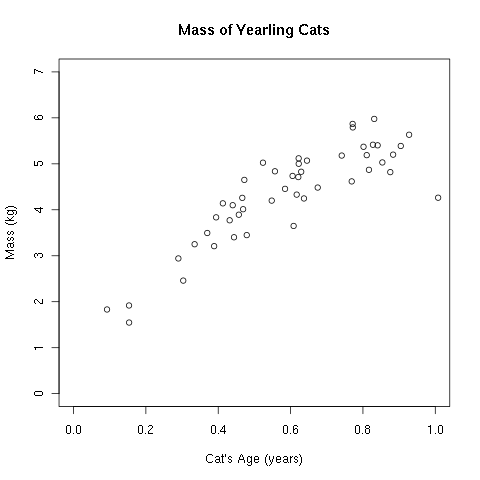
\includegraphics[width=6cm]{img/catsmass}
  }

  \vfill


\end{frame}


\begin{frame}
  \frametitle{Bivariate Data}

  What if we change it a little bit: \\
  \begin{tabular}{r@{~$=$~}l}
    $x$ & Age of Cat (between 0 and 20 years)  \\
    $y$ & Mass of Cat (kg)
  \end{tabular}
  
  \vfill

  \only<2->
  {

    As the age of the cat increases in the first year we expect that
    the cat's mass will \textbf{tend} to increase, but eventually it
    will level out.

  }

  \only<3->
  {
    \includegraphics[width=6cm]{img/catsmassLater}
  }

  \vfill


\end{frame}


\begin{frame}
  Question: How do we quantify the ``tendency'' of this relationship?
\end{frame}


\subsection{Correlation}


\begin{frame}
  \frametitle{Define the terms}

  \begin{columns}
    \column{.25\textwidth}

    \begin{tabular}{l|l}
      $X$ & $Y$ \\ \hline
      $x_1$ & $y_1$ \\
      $x_2$ & $y_2$ \\
      $x_3$ & $y_3$ \\
      $x_4$ & $y_4$ \\
      $\vdots$ & $\vdots$ \\
      $x_n$ & $y_n$ \\
    \end{tabular}


    \vfill

    \column{.75\textwidth}

    \only<3->
    {
      There is a ``one to one'' correspondence between each
      row. i.e. $x_3$ and $y_3$ are related to one another.

    }

    \vfill

  \end{columns}


  \begin{columns}
    \column{.5\textwidth}

    \only<4-> {

      Examine $x$ by itself: \\
      \begin{tabular}{l}
        N \\
        $\bar{x}$ \\
        $s_x$
      \end{tabular}

      Standard statistics.

    }
      
    \column{.5\textwidth}


    \only<5-> {

      Examine $y$ by itself: \\
      \begin{tabular}{l}
        N \\
        $\bar{y}$ \\
        $s_y$
      \end{tabular}

      Standard statistics.


    }


  \end{columns}


\end{frame}

\begin{frame}
  \frametitle{Example}

  \begin{columns}
    \column{.25\textwidth}

    \begin{tabular}{l|l}
      $X$ & $Y$ \\ \hline
      1 & 2 \\
      2 & 4  \\
      3 & 9 \\
      4 & 12
    \end{tabular}


    \vfill

    \column{.75\textwidth}

    \only<4->
    {
      \includegraphics[width=4cm]{img/simpleCorrelationExample}
    }

    \vfill

  \end{columns}


  \begin{columns}
    \column{.5\textwidth}

    \only<2-> {

      Examine $x$ by itself: \\
      \begin{tabular}{l}
        $N=4$ \\
        $\bar{x}=2.5$ \\
        $s_x=1.29$
      \end{tabular}


    }
      
    \column{.5\textwidth}


    \only<3-> {

      Examine $y$ by itself: \\
      \begin{tabular}{l}
        $n=4$ \\
        $\bar{y}=6.75$ \\
        $s_y=4.57$
      \end{tabular}



    }


  \end{columns}


\end{frame}

\begin{frame}{Now Bring Them Together}

  Graphically, we can look at the scatter plot:

  \includegraphics[height=4cm]{img/correlation09}
  
\end{frame}



\begin{frame}{Positive vs. Negative Relationships}

  \begin{columns}
    \column{.45\textwidth}

    \begin{definition}
      If $y$ \textbf{tends} to increase as $x$ increases then we say
      that it is a \textit{positive relationship} : \\
      \centerline{\includegraphics[width=5cm]{img/positiveRelationship}}
    \end{definition}

    \column{.5\textwidth}

    \begin{definition}
      If $y$ \textbf{tends} to decrease as $x$ increases then we say
      that it is a \textit{negative relationship} : \\
      \centerline{\includegraphics[width=5cm]{img/negativeRelationship}}
    \end{definition}

  \end{columns}
  
\end{frame}


\begin{frame}{Calculating the Correlation}

  First define the following sums:
  \begin{eqnarray*}
    S_{xx} & = & (x_1-\bar{x})^2 + (x_2-\bar{x})^2 + \cdot + (x_n-\bar{x})^2, \\
    S_{yy} & = & (y_1-\bar{y})^2 + (y_2-\bar{y})^2 + \cdot + (y_n-\bar{y})^2, \\
    S_{xy} & = & (x_1-\bar{x}) + (x_2-\bar{x}) + \cdot + (x_n-\bar{x}), \\
  \end{eqnarray*}

  \uncover<2->
  {
    
    \begin{definition}{Sample Correlation}
      The sample correlation coefficient is defined to be
      \begin{eqnarray*}
        r & = & \frac{S_{xy}}{\sqrt{S_{xx} S_{yy}}}.
      \end{eqnarray*}
    \end{definition}

  }
  
\end{frame}


\begin{frame}
  \frametitle{Example}
  \vspace*{-1em}
  \begin{columns}
    \column{.25\textwidth}

    \begin{tabular}{l|l}
      $X$ & $Y$ \\ \hline
      1 & 2 \\
      2 & 4  \\
      3 & 9 \\
      4 & 12
    \end{tabular}


    \vfill

    \column{.75\textwidth}

    \only<2->
    {
      \begin{eqnarray*}
        \bar{x} & = & 2.5 \\
        \bar{y} & = & 6.75
      \end{eqnarray*}
    }

    \vfill

  \end{columns}

  \only<3->
  {
    \begin{eqnarray*}
      s_{xx} & = & \lp 1-2.5\rp^2 + \lp 2 - 2.5 \rp^2 + \lp 3 - 2.5 \rp^2 + \lp 4 - 2.5 \rp^2 \\
            & = & 5, \\
      s_{yy} & = & \lp 2-6.75\rp^2 + \lp 4 - 6.75 \rp^2 + \lp 9 - 6.75 \rp^2 + \lp 12 - 6.75 \rp^2 \\
            & = & 62.75, \\
      s_{xx} & = & \lp 1-2.5\rp\lp 2-6.75\rp + \lp 2 - 2.5 \rp\lp 4 - 6.75 \rp + \lp 3 - 2.5 \rp\lp 9 - 6.75 \rp + \lp 4 - 2.5 \rp\lp 12 - 6.75 \rp \\
            & = & 17.5
    \end{eqnarray*}
  } 

  \only<4->
  {
    \begin{eqnarray*}
      r & = & \frac{17.5}{\sqrt{5\cdot 62.75}}, \\
        & \approx & 0.988
    \end{eqnarray*}
  }


\end{frame}



\begin{frame}{Correlation}

  \hspace*{-3em}
  \begin{tabular}{rrr}
    \includegraphics[height=4cm]{img/correlation09} & 
    \includegraphics[height=4cm]{img/correlation05} &
    \includegraphics[height=4cm]{img/correlation0} \\
    \includegraphics[height=4cm]{img/correlation-05} &
    \includegraphics[height=4cm]{img/correlation-09}
  \end{tabular}


\end{frame}


\begin{frame}
  \frametitle{Inference on the Correlation}

  \begin{definition}
    The sample correlation can be used to define a $t$-distribution:
    \begin{eqnarray*}
      t & = & \frac{r\sqrt{n-2}}{\sqrt{1-r^2}}
    \end{eqnarray*}
    with $n-2$ degrees of freedom.
  \end{definition}

\end{frame}

\begin{frame}{Hypothesis Test for the Correlation}

  Is there a relationship between the two variables? \\
  \begin{tabular}{ll}
    $H_0$ & $r=0$, \\
    $H_a$ & $r\neq 0$.
  \end{tabular}

  (Note, a one sided test can also be constructed if you ask if there
  is a positive or negative relationship between the variables.)

  
\end{frame}


\begin{frame}{Clicker Quiz}

  \iftoggle{clicker}{%


    \begin{columns}
      \column{.25\textwidth}

      \begin{tabular}{l|l}
        $X$ & $Y$ \\ \hline
        1 & 2 \\
        2 & 4  \\
        3 & 9 \\
        4 & 12
      \end{tabular}


      \vfill

      \column{.75\textwidth}
      
      \begin{tabular}{ll}
        $H_0$ & $r=0$, \\
        $H_a$ & $r\neq 0$.
      \end{tabular} \\
      Use a 95\% confidence level.

    \vfill

  \end{columns}


    \vfill 


    \begin{tabular}{l@{\hspace{3em}}l@{\hspace{3em}}l@{\hspace{3em}}l}
      A: Reject $H_0$  & B: Do not reject $H_0$
    \end{tabular}

    \vfill
    \vfill
    \vfill

  }

\end{frame}


% LocalWords:  Clarkson pausesection hideallsubsections



\lecture{Regression Analysis}{regression-analysis}
\section{Regression Analysis}

\title{Regression Analysis}
\subtitle{Analysis Of The Slope Of The Regression Line}

\author{Kelly Black}
\institute{Clarkson University}
\date{18 April 2012}

\begin{frame}
  \titlepage
\end{frame}

\begin{frame}
  \frametitle{Outline}
  \tableofcontents[pausesection,hideothersubsections,sectionstyle=show/hide]
\end{frame}


\subsection{Clicker Quiz}


\begin{frame}
  \frametitle{Clicker Quiz}

    \iftoggle{clicker}{%

    \begin{columns}
      \column{.25\textwidth}

      \begin{tabular}{l|l}
        $X$ & $Y$ \\ \hline
        1 & 2 \\
        2 & 3  \\
        3 & 3 \\
        4 & 5  \\
        5 & 4
      \end{tabular}

      \column{.75\textwidth}

      Is there a relationship between the two variables? (Use a 95\%
      confidence level.)

      \begin{tabular}{l@{\hspace{3em}}l@{\hspace{3em}}l@{\hspace{3em}}l}
        A: Reject $H_0$  & B: Do not reject $H_0$
      \end{tabular}


      \begin{eqnarray*}
        \bar{x} & = & 3 \\
        \bar{y} & = & 3.4
      \end{eqnarray*}

    \end{columns}

      \begin{eqnarray*}
        s_{xx} & = & \lp 1-3\rp^2 + \lp 2 - 3 \rp^2 + \lp 3 - 3 \rp^2 + \lp 4 - 3 \rp^2 + \lp 5 - 3 \rp^2 \\
        & = & 10, \\
        s_{yy} & = & \lp 2-3.4\rp^2 + \lp 3 - 3.4 \rp^2 + \lp 3 - 3.4 \rp^2 + \lp 5 - 3.4 \rp^2 + \lp 4 - 3.4 \rp^2 \\
        & = & 5.2, \\
        s_{xy} & = & \lp 1-3\rp\lp 2-3.4\rp + \lp 2 - 3 \rp\lp 3 - 3.4 \rp + \lp 3 - 3 \rp\lp 3 - 3.4 \rp + \lp 4 - 3 \rp\lp 5 - 3.4 \rp + \lp 5-4 \rp \lp 4-3.4 \rp \\
        & = & 6
      \end{eqnarray*}

    \vfill 




    }

\end{frame}




\subsection{Linear Regression}

\begin{frame}
  \frametitle{Linear Regression}

    \begin{columns}
      \column{.65\textwidth}

      \centerline{\includegraphics[width=6cm]{img/regressionGeneral}}

      \column{.35\textwidth}
      
      from section 3.3 (second week)
      \begin{eqnarray*}
        \hat{m} & = & \frac{s_{xy}}{s_{xx}}, \\
        \hat{b} & = & \bar{y} - \hat{m} \bar{x}.
      \end{eqnarray*}

    \end{columns}

\end{frame}


\begin{frame}{The Residual}

  \begin{definition}
    The \textit{predicted value} for $y$ at $x$ is
    \begin{eqnarray*}
      \hat{y} & = & \hat{m} x + \hat{b}.
    \end{eqnarray*}

    The \textit{residual} at $x_i$ is 
    \begin{eqnarray*}
      \mathrm{Residual} & = & y_i - \lp \hat{m} x + \hat{b} \rp, \\
      & = & y_i - \hat{y}_i.
    \end{eqnarray*}

  \end{definition}

  \only<2->
  {

    \begin{definition}
      The variance of the error is 
      \begin{eqnarray*}
        s^2_y & = & \frac{\lp y_1 - \hat{y}_1\rp^2 + \lp y_2 - \hat{y}_2\rp^2 + \cdots + \lp y_n - \hat{y}_n\rp^2 }{n-2}.
      \end{eqnarray*}
    \end{definition}

  }
  
\end{frame}

\begin{frame}{Example}

    \begin{columns}
      \column{.25\textwidth}

      \begin{tabular}{l|l}
        $X$ & $Y$ \\ \hline
        1 & 2 \\
        2 & 3  \\
        3 & 3 \\
        4 & 5  \\
        5 & 4
      \end{tabular}

      \column{.65\textwidth}

      \begin{eqnarray*}
        \bar{x} & = & 3 \\
        \bar{y} & = & 3.4 \\
        s_{xx} & = & 10, \\
        s_{yy} & = & 5.2, \\
        s_{xx} & = & 6
      \end{eqnarray*}

      \end{columns}

  \only<2->
  {

    \begin{eqnarray*}
      \hat{m} & = & \frac{s_{xy}}{s_{xx}}, \\
      & = & 0.6, \\
      \hat{b} & = & \bar{y} - \hat{m} \bar{x}, \\
      & = & 1.6
    \end{eqnarray*}

  }

  
\end{frame}



\begin{frame}{Example}

    \begin{columns}
      \column{.25\textwidth}

      \begin{tabular}{l|l}
        $X$ & $Y$ \\ \hline
        1 & 2 \\
        2 & 3  \\
        3 & 3 \\
        4 & 5  \\
        5 & 4
      \end{tabular}

      \column{.65\textwidth}

      \begin{eqnarray*}
        \bar{x} & = & 3 \\
        \bar{y} & = & 3.4 \\
        s_{xx} & = & 10, \\
        s_{yy} & = & 5.2, \\
        s_{xx} & = & 6, \\
        \hat{m} & = & 0.6, \\
        \hat{b} & = & 1.6
      \end{eqnarray*}

      \end{columns}

  \only<2->
  {

      \begin{tabular}{r|r<{\onslide<3->}|r<{\onslide<4->}|r<{\onslide}} % 
        $X$ & $Y$ & $\hat{Y}$ & Residual \\ \hline
        1 & 2 & 2.2 & -.2 \\
        2 & 3 & 2.8 &  .2 \\
        3 & 3 & 3.4 & -.4 \\
        4 & 5 & 4.0 & 1.0  \\
        5 & 4 & 4.6 & -.6
      \end{tabular}


  }

  
\end{frame}


\begin{frame}{Example}

  \begin{tabular}{r|r|r|r}
    $X$ & $Y$ & $\hat{Y}$ & Residual \\ \hline
    1 & 2 & 2.2 & -.2 \\
    2 & 3 & 2.8 &  .2 \\
    3 & 3 & 3.4 & -.4 \\
    4 & 5 & 4.0 & 1.0  \\
    5 & 4 & 4.6 & -.6
  \end{tabular}

  \begin{eqnarray*}
    s^2_y & = & \frac{ (-.2)^2 + (.2)^2 + (-.4)^2 + (1.0)^2 + (-.6)^2}{5-2}, \\
    & = & \frac{1.6}{3}, \\
    s_y & = & \sqrt{\frac{1.6}{3}}, \\
    & \approx & .730
  \end{eqnarray*}
  
\end{frame}
  

\subsection{Inference for the Slope}

\begin{frame}
  \frametitle{Inference for the Slope}

  We have the following estimate for the linear regression line:
  \begin{eqnarray*}
    y & = & \hat{m} x + \hat{b}.
  \end{eqnarray*}

  \begin{definition}
    The regression estimate for the slope satisfies the $t$ distribution
    \begin{eqnarray*}
      t & = & \frac{\hat{m}-m}{s_y}
    \end{eqnarray*}
    with $n-2$ degrees of freedom.
  \end{definition}

\end{frame}


\begin{frame}{Inference for the Slope}

  \begin{columns}

    \column{.5\textwidth}
    Confidence Intervals:
    \begin{eqnarray*}
      t^* & = & \frac{\mathrm{error}}{s_y}
    \end{eqnarray*}
    with $n-2$ degrees of freedom.

    \column{.5\textwidth}

    Hypothesis Testing:
    \begin{eqnarray*}
      t & = & \frac{\hat{m}-m}{s_y}
    \end{eqnarray*}
    with $n-2$ degrees of freedom.

    
  \end{columns}

\end{frame}

\begin{frame}
  \frametitle{Clicker Quiz}

    \iftoggle{clicker}{%

    \begin{columns}
      \column{.15\textwidth}

      \begin{tabular}{l|l}
        $X$ & $Y$ \\ \hline
        1 & 2 \\
        2 & 3  \\
        3 & 3 \\
        4 & 5  \\
        5 & 4
      \end{tabular}

      \column{.25\textwidth}

      \begin{eqnarray*}
        \hat{m} & = & 0.6, \\
        \hat{b} & = & 1.6, \\
        s_y & = & .730
      \end{eqnarray*}


      \column{.6\textwidth}

      Is the slope different from zero? (Use a 95\% confidence level.)

    \end{columns}

    \vfill

    \begin{tabular}{l@{\hspace{3em}}l@{\hspace{3em}}l@{\hspace{3em}}l}
      A: Reject $H_0$  & B: Do not reject $H_0$
    \end{tabular}

    \vfill

    }

\end{frame}


% LocalWords:  Clarkson pausesection hideallsubsections



\lecture{Inference On The Slope}{inference-slope}
\section{The Lecture}


\title{Estimating The Slope}
\subtitle{Inference on the Slope}

\author{Kelly Black}
\institute{Clarkson University}
\date{20 April 2012}

\begin{frame}
  \titlepage
\end{frame}

\begin{frame}
  \frametitle{Outline}
  \tableofcontents[pausesection,hideothersubsections,sectionstyle=show/hide]
\end{frame}


\subsection{Overview of Regression}


\begin{frame}
  \frametitle{Linear Regression}


  \begin{tabular}{r|r<{\onslide<2->}|r<{\onslide<3->}|r<{\onslide}} % 
    $X$ & $Y$ & $\hat{Y}$ & Residual \\ \hline
    $x_1$ & $y_1$ & $\hat{y}_1=\hat{m}x_1+\hat{b}$ & $\epsilon_1 = y_1-\hat{y}_1$ \\
    $x_2$ & $y_2$ & $\hat{y}_2=\hat{m}x_2+\hat{b}$ & $\epsilon_2 = y_2-\hat{y}_2$  \\
    $\vdots$ & $\vdots$ & $\vdots$ & $\vdots$  \\
    $x_n$ & $y_n$ & $\hat{y}_n=\hat{m}x_n+\hat{b}$ & $\epsilon_n = y_n-\hat{y}_n$
  \end{tabular}

  Calculate the following:
  \begin{eqnarray*}
    S_{xx}, \\
    S_{yy}, \\
    S_{xy}, \\
    \hat{m} & = & \frac{S_{xy}}{S_{yy}}, \\
    \hat{b} & = & \bar{y} - \hat{m} \bar{x}, \\
    \only<4->
    {
      s^2_y & = & \frac{\lp y_1 - \hat{y}_1\rp^2 + \lp y_2 - \hat{y}_2\rp^2 + \cdots + \lp y_n - \hat{y}_n\rp^2 }{n-2}.
    }
  \end{eqnarray*}

\end{frame}



\begin{frame}{What is the relationship?}


    \begin{columns}
      \column{.33\textwidth}

      \begin{eqnarray*}
        H_0: & & m=0, \\
        H_a: & & m<0,
      \end{eqnarray*}
      a negative relationship?

      \column{.33\textwidth}

      \begin{eqnarray*}
        H_0: & & m=0, \\
        H_a: & & m>0,
      \end{eqnarray*}
      a positive relationship?


      \column{.33\textwidth}

      \begin{eqnarray*}
        H_0: & & m=0, \\
        H_a: & & m\neq 0,
      \end{eqnarray*}
      any relationship?

      
    \end{columns}

  
\end{frame}

\begin{frame}
  \frametitle{Inference for the Slope}

  We have the following estimate for the linear regression line:
  \begin{eqnarray*}
    y & = & \hat{m} x + \hat{b}.
  \end{eqnarray*}

  \begin{definition}
    The regression estimate for the slope satisfies the $t$ distribution
    \begin{eqnarray*}
      t & = & \frac{\hat{m}-m}{s_y}
    \end{eqnarray*}
    with $n-2$ degrees of freedom.
  \end{definition}

  \begin{columns}

    \column{.5\textwidth}
    Confidence Intervals:
    \begin{eqnarray*}
      t^* & = & \frac{\mathrm{error}}{s_y}
    \end{eqnarray*}
    with $n-2$ degrees of freedom.

    \column{.5\textwidth}

    Hypothesis Testing:
    \begin{eqnarray*}
      t & = & \frac{\hat{m}-m}{s_y}
    \end{eqnarray*}
    with $n-2$ degrees of freedom.

    
  \end{columns}

\end{frame}


\begin{frame}

    \iftoggle{clicker}{%

    \begin{columns}
      \column{.25\textwidth}

      \begin{tabular}{l|l}
        $X$ & $Y$ \\ \hline
        1 & 3 \\
        2 & 5  \\
        3 & 9 \\
        4 & 7  \\
        5 & 10
      \end{tabular}

      \column{.75\textwidth}

      Find the 95\% confidence interval for the slope.

      \begin{tabular}{l@{\hspace{3em}}l@{\hspace{3em}}l@{\hspace{3em}}l}
        A: -4.3 to 7.5  & B: -10.0 to 13.2 \\ C: -11.6 to 14.8
      \end{tabular}


      \begin{eqnarray*}
        \bar{x} & = & 3 \\
        \bar{y} & = & 6.8, \\
        s_y & = & 4.16
      \end{eqnarray*}

    \end{columns}

      \begin{eqnarray*}
        s_{xx} & = & \lp 1-3\rp^2 + \lp 2 - 3 \rp^2 + \lp 3 - 3 \rp^2 + \lp 4 - 3 \rp^2 + \lp 5 - 3 \rp^2 \\
        & = & 10, \\
        s_{yy} & = & \lp 3-6.8\rp^2 + \lp 5 - 6.8 \rp^2 + \lp 9 - 6.8 \rp^2 + \lp 7 - 6.8 \rp^2 + \lp 10 - 6.8 \rp^2 \\
        & = & 32.8, \\
        s_{xy} & = & \lp 1-3\rp\lp 3-6.8\rp + \lp 2 - 3 \rp\lp 5 - 6.8 \rp + \lp 3 - 3 \rp\lp 9 - 6.8 \rp + \lp 4 - 3 \rp\lp 7 - 6.8 \rp + \lp 5-4 \rp \lp 10-6.8 \rp \\
        & = & 16
      \end{eqnarray*}

    \vfill 




    }

\end{frame}


\subsection{Inference On Predicted Value}

\begin{frame}{The Predicted Value}

  \begin{definition}
    The \textit{predicted value} for $y$ at $x$ is
    \begin{eqnarray*}
      \hat{y} & = & \hat{m} x + \hat{b}.
    \end{eqnarray*}

    The \textit{residual} at $x_i$ is 
    \begin{eqnarray*}
      \mathrm{Residual} & = & y_i - \lp \hat{m} x + \hat{b} \rp, \\
      & = & y_i - \hat{y}_i.
    \end{eqnarray*}

  \end{definition}

  
\end{frame}

\begin{frame}
  \frametitle{The Predicted Value}

  The predicted value is 
  \begin{eqnarray*}
    \hat{y} & = & \hat{m} x + \hat{b}.
  \end{eqnarray*}


  The predicted value  satisfies a $t$-distribution by
  \begin{eqnarray*}
    t & = & \frac{\hat{y}-y_{\mathrm{true}}}{s_y \sqrt{\frac{1}{n}+\frac{(x_y-\bar{x})^2}{S_{xx}}}},
  \end{eqnarray*}
  with $n-2$ degrees of freedom.

  \only<2->
  {

    \begin{columns}

      \column{.5\textwidth}
      Confidence Intervals:
      \begin{eqnarray*}
        t & = & \frac{\mathrm{error}}{s_y \sqrt{\frac{1}{n}+\frac{(x_y-\bar{x})^2}{S_{xx}}}},
      \end{eqnarray*}
      with $n-2$ degrees of freedom.

      \column{.5\textwidth}

      Hypothesis Testing:
      \begin{eqnarray*}
        t & = & \frac{\hat{y}-y_{\mathrm{true}}}{s_y \sqrt{\frac{1}{n}+\frac{(x_y-\bar{x})^2}{S_{xx}}}},
      \end{eqnarray*}
      with $n-2$ degrees of freedom.

    
    \end{columns}
  }


\end{frame}


\begin{frame}{Example}


    \begin{columns}
      \column{.15\textwidth}

      \begin{tabular}{l|l}
        $X$ & $Y$ \\ \hline
        1 & 3 \\
        2 & 5  \\
        3 & 9 \\
        4 & 7  \\
        5 & 10
      \end{tabular}

      \column{.44\textwidth}

      \begin{eqnarray*}
        \bar{x} & = & 3 \\
        \bar{y} & = & 6.8, \\
        s_y & = & 4.16 \\
        \hat{m} & = & 1.6, \\
        \hat{b} & = & 2.0.
      \end{eqnarray*}

      \column{.44\textwidth}

      \begin{eqnarray*}
        s_{xx} & = & 10, \\
        s_{yy} & = & 32.8, \\
        s_{xy} & = & 16.
      \end{eqnarray*}

    \end{columns}


    \vfill 


      Find the 95\% confidence interval for the value of $y$ at $x=3.5$.

      \only<2->
      {

        The 95\% confidence interval for the value of $y$ at $x=3.5$
        is between 1.33 and 13.87 assuming a $t$-distribution with 3 d.f..
      }


\end{frame}


\begin{frame}{Example}

  \iftoggle{clicker}{%

    \begin{columns}
      \column{.15\textwidth}

      \begin{tabular}{l|l}
        $X$ & $Y$ \\ \hline
        1 & 3 \\
        2 & 5  \\
        3 & 9 \\
        4 & 7  \\
        5 & 10
      \end{tabular}

      \column{.44\textwidth}

      \begin{eqnarray*}
        \bar{x} & = & 3 \\
        \bar{y} & = & 6.8, \\
        s_y & = & 4.16 \\
        \hat{m} & = & 1.6, \\
        \hat{b} & = & 2.0.
      \end{eqnarray*}

      \column{.44\textwidth}

      \begin{eqnarray*}
        s_{xx} & = & 10, \\
        s_{yy} & = & 32.8, \\
        s_{xy} & = & 16.
      \end{eqnarray*}

    \end{columns}


    \vfill 


      Find the 95\% confidence interval for the value of $y$ at
      $x=4.5$.

      \vfill

      \begin{tabular}{l@{\hspace{3em}}l@{\hspace{3em}}l@{\hspace{3em}}l}
        A: .58 to 17.8  & B: 5.3 to 13.0 & C: 1.7 to 16.7
      \end{tabular}


    }

\end{frame}


% LocalWords:  Clarkson pausesection hideallsubsections





\end{document}

% LocalWords:  Clarkson pausesection hideallsubsections
